\documentclass[]{book}
\usepackage{lmodern}
\usepackage{amssymb,amsmath}
\usepackage{ifxetex,ifluatex}
\usepackage{fixltx2e} % provides \textsubscript
\ifnum 0\ifxetex 1\fi\ifluatex 1\fi=0 % if pdftex
  \usepackage[T1]{fontenc}
  \usepackage[utf8]{inputenc}
\else % if luatex or xelatex
  \ifxetex
    \usepackage{mathspec}
  \else
    \usepackage{fontspec}
  \fi
  \defaultfontfeatures{Ligatures=TeX,Scale=MatchLowercase}
\fi
% use upquote if available, for straight quotes in verbatim environments
\IfFileExists{upquote.sty}{\usepackage{upquote}}{}
% use microtype if available
\IfFileExists{microtype.sty}{%
\usepackage{microtype}
\UseMicrotypeSet[protrusion]{basicmath} % disable protrusion for tt fonts
}{}
\usepackage{hyperref}
\hypersetup{unicode=true,
            pdftitle={Validation Report for adoptr package},
            pdfauthor={Kevin Kunzmann \& Maximilian Pilz},
            pdfborder={0 0 0},
            breaklinks=true}
\urlstyle{same}  % don't use monospace font for urls
\usepackage{natbib}
\bibliographystyle{apalike}
\usepackage{color}
\usepackage{fancyvrb}
\newcommand{\VerbBar}{|}
\newcommand{\VERB}{\Verb[commandchars=\\\{\}]}
\DefineVerbatimEnvironment{Highlighting}{Verbatim}{commandchars=\\\{\}}
% Add ',fontsize=\small' for more characters per line
\usepackage{framed}
\definecolor{shadecolor}{RGB}{248,248,248}
\newenvironment{Shaded}{\begin{snugshade}}{\end{snugshade}}
\newcommand{\AlertTok}[1]{\textcolor[rgb]{0.94,0.16,0.16}{#1}}
\newcommand{\AnnotationTok}[1]{\textcolor[rgb]{0.56,0.35,0.01}{\textbf{\textit{#1}}}}
\newcommand{\AttributeTok}[1]{\textcolor[rgb]{0.77,0.63,0.00}{#1}}
\newcommand{\BaseNTok}[1]{\textcolor[rgb]{0.00,0.00,0.81}{#1}}
\newcommand{\BuiltInTok}[1]{#1}
\newcommand{\CharTok}[1]{\textcolor[rgb]{0.31,0.60,0.02}{#1}}
\newcommand{\CommentTok}[1]{\textcolor[rgb]{0.56,0.35,0.01}{\textit{#1}}}
\newcommand{\CommentVarTok}[1]{\textcolor[rgb]{0.56,0.35,0.01}{\textbf{\textit{#1}}}}
\newcommand{\ConstantTok}[1]{\textcolor[rgb]{0.00,0.00,0.00}{#1}}
\newcommand{\ControlFlowTok}[1]{\textcolor[rgb]{0.13,0.29,0.53}{\textbf{#1}}}
\newcommand{\DataTypeTok}[1]{\textcolor[rgb]{0.13,0.29,0.53}{#1}}
\newcommand{\DecValTok}[1]{\textcolor[rgb]{0.00,0.00,0.81}{#1}}
\newcommand{\DocumentationTok}[1]{\textcolor[rgb]{0.56,0.35,0.01}{\textbf{\textit{#1}}}}
\newcommand{\ErrorTok}[1]{\textcolor[rgb]{0.64,0.00,0.00}{\textbf{#1}}}
\newcommand{\ExtensionTok}[1]{#1}
\newcommand{\FloatTok}[1]{\textcolor[rgb]{0.00,0.00,0.81}{#1}}
\newcommand{\FunctionTok}[1]{\textcolor[rgb]{0.00,0.00,0.00}{#1}}
\newcommand{\ImportTok}[1]{#1}
\newcommand{\InformationTok}[1]{\textcolor[rgb]{0.56,0.35,0.01}{\textbf{\textit{#1}}}}
\newcommand{\KeywordTok}[1]{\textcolor[rgb]{0.13,0.29,0.53}{\textbf{#1}}}
\newcommand{\NormalTok}[1]{#1}
\newcommand{\OperatorTok}[1]{\textcolor[rgb]{0.81,0.36,0.00}{\textbf{#1}}}
\newcommand{\OtherTok}[1]{\textcolor[rgb]{0.56,0.35,0.01}{#1}}
\newcommand{\PreprocessorTok}[1]{\textcolor[rgb]{0.56,0.35,0.01}{\textit{#1}}}
\newcommand{\RegionMarkerTok}[1]{#1}
\newcommand{\SpecialCharTok}[1]{\textcolor[rgb]{0.00,0.00,0.00}{#1}}
\newcommand{\SpecialStringTok}[1]{\textcolor[rgb]{0.31,0.60,0.02}{#1}}
\newcommand{\StringTok}[1]{\textcolor[rgb]{0.31,0.60,0.02}{#1}}
\newcommand{\VariableTok}[1]{\textcolor[rgb]{0.00,0.00,0.00}{#1}}
\newcommand{\VerbatimStringTok}[1]{\textcolor[rgb]{0.31,0.60,0.02}{#1}}
\newcommand{\WarningTok}[1]{\textcolor[rgb]{0.56,0.35,0.01}{\textbf{\textit{#1}}}}
\usepackage{longtable,booktabs}
\usepackage{graphicx,grffile}
\makeatletter
\def\maxwidth{\ifdim\Gin@nat@width>\linewidth\linewidth\else\Gin@nat@width\fi}
\def\maxheight{\ifdim\Gin@nat@height>\textheight\textheight\else\Gin@nat@height\fi}
\makeatother
% Scale images if necessary, so that they will not overflow the page
% margins by default, and it is still possible to overwrite the defaults
% using explicit options in \includegraphics[width, height, ...]{}
\setkeys{Gin}{width=\maxwidth,height=\maxheight,keepaspectratio}
\IfFileExists{parskip.sty}{%
\usepackage{parskip}
}{% else
\setlength{\parindent}{0pt}
\setlength{\parskip}{6pt plus 2pt minus 1pt}
}
\setlength{\emergencystretch}{3em}  % prevent overfull lines
\providecommand{\tightlist}{%
  \setlength{\itemsep}{0pt}\setlength{\parskip}{0pt}}
\setcounter{secnumdepth}{5}
% Redefines (sub)paragraphs to behave more like sections
\ifx\paragraph\undefined\else
\let\oldparagraph\paragraph
\renewcommand{\paragraph}[1]{\oldparagraph{#1}\mbox{}}
\fi
\ifx\subparagraph\undefined\else
\let\oldsubparagraph\subparagraph
\renewcommand{\subparagraph}[1]{\oldsubparagraph{#1}\mbox{}}
\fi

%%% Use protect on footnotes to avoid problems with footnotes in titles
\let\rmarkdownfootnote\footnote%
\def\footnote{\protect\rmarkdownfootnote}

%%% Change title format to be more compact
\usepackage{titling}

% Create subtitle command for use in maketitle
\providecommand{\subtitle}[1]{
  \posttitle{
    \begin{center}\large#1\end{center}
    }
}

\setlength{\droptitle}{-2em}

  \title{Validation Report for \textbf{adoptr} package}
    \pretitle{\vspace{\droptitle}\centering\huge}
  \posttitle{\par}
    \author{Kevin Kunzmann \& Maximilian Pilz}
    \preauthor{\centering\large\emph}
  \postauthor{\par}
      \predate{\centering\large\emph}
  \postdate{\par}
    \date{2019-07-05}

\usepackage{booktabs}

\begin{document}
\maketitle

{
\setcounter{tocdepth}{1}
\tableofcontents
}
\hypertarget{introduction}{%
\chapter{Introduction}\label{introduction}}

This work is licensed under the \href{https://creativecommons.org/licenses/by-sa/4.0/deed.en}{CC-BY-SA 4.0 license}

\hypertarget{preliminaries}{%
\section{Preliminaries}\label{preliminaries}}

R package validation for regulatory environments can be a
tedious endeavour.
The authors firmly believe that under the current regulation,
there is no such thing as a `validated R package':
validation is by definition a process conducted by the \emph{user}.
This validation report merely aims at facilitating
validation of \textbf{\href{https://github.com/kkmann/adoptr}{adoptr}} as
much as possible.
No warranty whatsoever as to the correctness of \textbf{adoptr} nor the
completeness of the validation report are given by the authors.

We assume that the reader is familiar with the notation an theoretical
background of \textbf{adoptr}.
Otherwise, the following resources might be of help:

\begin{itemize}
\tightlist
\item
  \textbf{adoptr} online documentation at \url{https://kkmann.github.io/adoptr/}
\item
  paper on the theoretical background of the core \textbf{adoptr} functionality \citep{variational}
\item
  a general overview on adaptive designs is given in \citep{Bauer2015}
\item
  a more extensive treatment of the subject in \citep{Wassmer2016}.
\end{itemize}

\hypertarget{scope}{%
\section{Scope}\label{scope}}

\textbf{adoptr} itself already makes extensive use of unittesting to
ensure correctness of all implemented functions.
Yet, due to constraints on the build-time for an R package,
the range of scenarios covered in the unittests of \textbf{adoptr} is
rather limited.
Furthermore, the current R unittesting framework does not permit
an easy generation of a human-readable report of the test cases
to acertain coverage and test quality.
Therefore, \textbf{adoptr} splits testing in two parts: technical
correctness is ensured via an extensive unittesting suit in \textbf{adoptr}
itself (aiming to maintain a 100\% code coverage).

The validation report, however, runs through a wide range of possible
application scenarios and ensures plausibility of results as well
as consistency with existing methods wherever possible.
The report itself is implemented as a collection of Rmarkdown documents
allowing to show both the underlying code as well as the corresponding
output in a human-readable format.

The online version of the report is dynamically re-generated on a
daily basis using the Travis-CI service based on the respective
most current version of \textbf{adoptr} on CRAN.
The result of this daily build is available at
\url{https://kkmann.github.io/adoptr-validation-report/}.
To ensure early warning in case of any test-case failures,
formal tests are implemented using the \textbf{testthat} package
\citep{R-testthat}.
I.e., the combination of using a unittesting framework, a continuous
integration, and continuous deployment service leads to an always
up-to-date validation report (build on the current R release on Linux).
Any failure of the integrated formal tests will cause the build status
of the validation report to switch from `passing' to `failed' and
the respective maintainer will be notified immediately.

\hypertarget{validating-a-local-installation-of-adoptr}{%
\subsection{Validating a local installation of adoptr}\label{validating-a-local-installation-of-adoptr}}

Note that, strictly speaking, the online version of the validation
report only provides evidence of the correctness on the respective
Travis-CI cloud virtual machine infrastructure using the respective
most recent release of R and the most recent versions of the
dependencies available on CRAN.
In some instances it might therefore be desireable to conduct a
local validaton of \textbf{adoptr}.

To do so, one should install \textbf{adoptr} with the \texttt{INSTALL\_opts} option
to include tests and invoke the test suit locally via

\begin{Shaded}
\begin{Highlighting}[]
\KeywordTok{install.packages}\NormalTok{(}\StringTok{"adoptr"}\NormalTok{, }\DataTypeTok{INSTALL_opts =} \KeywordTok{c}\NormalTok{(}\StringTok{"--install-tests"}\NormalTok{))}
\NormalTok{tools}\OperatorTok{::}\KeywordTok{testInstalledPackage}\NormalTok{(}\StringTok{"adoptr"}\NormalTok{, }\DataTypeTok{types =} \KeywordTok{c}\NormalTok{(}\StringTok{"examples"}\NormalTok{, }\StringTok{"tests"}\NormalTok{))}
\end{Highlighting}
\end{Shaded}

Upon passing the test suit successfully, the validation report
can be build locally.
To do so, first clone the entire source directory and switch
to the newly created folder

\begin{Shaded}
\begin{Highlighting}[]
\FunctionTok{git}\NormalTok{ clone https://github.com/kkmann/adoptr-validation-report.git}
\BuiltInTok{cd}\NormalTok{ adoptr-validation-report}
\end{Highlighting}
\end{Shaded}

Make sure that all packages requied for building the report are
available, i.e., install all dependencies listed in the top-level
\texttt{DESCRIPTION} file, e.g.,

\begin{Shaded}
\begin{Highlighting}[]
\KeywordTok{install.packages}\NormalTok{(}\KeywordTok{c}\NormalTok{(}
    \StringTok{"adoptr"}\NormalTok{, }
    \StringTok{"tidyverse"}\NormalTok{, }
    \StringTok{"bookdown"}\NormalTok{, }
    \StringTok{"rpact"}\NormalTok{, }
    \StringTok{"testthat"}\NormalTok{, }
    \StringTok{"pwr"}\NormalTok{ ) )}
\end{Highlighting}
\end{Shaded}

The book can then be build using the terminal command

\begin{Shaded}
\begin{Highlighting}[]
\ExtensionTok{Rscript}\NormalTok{ -e }\StringTok{'bookdown::render_book("index.Rmd", output_format = "all")'}
\end{Highlighting}
\end{Shaded}

or directly from R via

\begin{Shaded}
\begin{Highlighting}[]
\NormalTok{bookdown}\OperatorTok{::}\KeywordTok{render_book}\NormalTok{(}\StringTok{"index.Rmd"}\NormalTok{, }\DataTypeTok{output_format =} \StringTok{"all"}\NormalTok{)}
\end{Highlighting}
\end{Shaded}

This produces a new folder \texttt{\_book} with the html and pdf versions
of the report.

\hypertarget{validation-scenarios}{%
\section{Validation Scenarios}\label{validation-scenarios}}

\hypertarget{scenario-i-large-effect-point-prior}{%
\subsection{\texorpdfstring{\protect\hyperlink{scenarioI}{Scenario I: Large effect, point prior}}{Scenario I: Large effect, point prior}}\label{scenario-i-large-effect-point-prior}}

This is the default scenario.

\begin{itemize}
\tightlist
\item
  \textbf{Data distribution:} Two-armed trial with normally distributed test statistic
\item
  \textbf{Prior:} \(\delta\sim\delta_{0.4}\)
\item
  \textbf{Null hypothesis:} \(\mathcal{H}_0:\delta \leq 0\)
\end{itemize}

\hypertarget{variant-i.1-minimizing-expected-sample-size-under-the-alternative}{%
\subsubsection{\texorpdfstring{\protect\hyperlink{variantI_1}{Variant I.1: Minimizing Expected Sample Size under the Alternative}}{Variant I.1: Minimizing Expected Sample Size under the Alternative}}\label{variant-i.1-minimizing-expected-sample-size-under-the-alternative}}

\begin{itemize}
\tightlist
\item
  \textbf{Objective:} \(ESS := \boldsymbol{E}\big[n(X_1)\,|\,\delta=0.4\big]\)
\item
  \textbf{Constraints:}

  \begin{enumerate}
  \def\labelenumi{\arabic{enumi}.}
  \tightlist
  \item
    \(Power := \boldsymbol{Pr}\big[c_2(X_1) < X_2\,|\,\delta=0.4\big] \geq 0.8\)
  \item
    \(TOER := \boldsymbol{Pr}\big[c_2(X_1) < X_2\,|\,\delta=0.0\big] \leq 0.025\)
  \item
    Three variants: two-stage, group-sequential, one-stage.
  \end{enumerate}
\item
  \textbf{Formal tests:}

  \begin{enumerate}
  \def\labelenumi{\arabic{enumi}.}
  \tightlist
  \item
    Number of iterations are checked against default maximum to ensure proper
    convergence.
  \item
    All three \textbf{adoptr} variants (two-stage, group-sequential, one-stage)
    comply with constraints. Internally validated by testing vs.~simulated
    values of the power curve at respective points.
  \item
    Is \(n()\) of the optimal two-stage design monotonously decreasing on
    continuation area?
  \item
    \(ESS\) of optimal two-stage design is lower than \(ESS\) of optimal
    group-sequential one and that is in turn lower than the one of the
    optimal one-stage design.
  \item
    \(ESS\) of optimal group-sequential design is lower than \(ESS\) of
    externally computed group-sequential design using the \href{https://rpact.org/}{rpact} package.
  \item
    Are the \(ESS\) values obtained from simulation the same as the ones
    obtained by using numerical integration via \texttt{adoptr::evaluate}?
  \end{enumerate}
\end{itemize}

\hypertarget{variant-i.2-minimizing-expected-sample-size-under-the-null-hypothesis}{%
\subsubsection{\texorpdfstring{\protect\hyperlink{variantI_2}{Variant I.2: Minimizing Expected Sample Size under the Null Hypothesis}}{Variant I.2: Minimizing Expected Sample Size under the Null Hypothesis}}\label{variant-i.2-minimizing-expected-sample-size-under-the-null-hypothesis}}

\begin{itemize}
\tightlist
\item
  \textbf{Objective:} \(ESS := \boldsymbol{E}\big[n(X_1)\,|\,\color{red}{\delta=0.0}\big]\)
\item
  \textbf{Constraints:}

  \begin{enumerate}
  \def\labelenumi{\arabic{enumi}.}
  \tightlist
  \item
    \(Power := \boldsymbol{Pr}\big[c_2(X_1) < X_2\,|\,\delta=0.4\big] \geq 0.8\)
  \item
    \(TOER := \boldsymbol{Pr}\big[c_2(X_1) < X_2\,|\,\delta=0.0\big] \leq 0.025\)
  \end{enumerate}
\item
  \textbf{Formal tests:}

  \begin{enumerate}
  \def\labelenumi{\arabic{enumi}.}
  \tightlist
  \item
    Number of iterations are checked against default maximum to ensure proper
    convergence.
  \item
    Validate constraint compliance by testing vs.~simulated
    values of the power curve at respective points.
  \item
    \(n()\) of optimal design is monotonously increasing on continuation area.
  \item
    \(ESS\) of optimal two-stage design is lower than \(ESS\) of externally
    computed group-sequential design using the \href{https://rpact.org/}{rpact} package.
  \item
    Are the \(ESS\) values obtained from simulation the same as the ones
    obtained by using numerical integration via \texttt{adoptr::evaluate}?
  \end{enumerate}
\end{itemize}

\hypertarget{variant-i.3-condtional-power-constraint}{%
\subsubsection{\texorpdfstring{\protect\hyperlink{variantI_3}{Variant I.3: Condtional Power Constraint}}{Variant I.3: Condtional Power Constraint}}\label{variant-i.3-condtional-power-constraint}}

\begin{itemize}
\tightlist
\item
  \textbf{Objective:} \(ESS := \boldsymbol{E}\big[n(X_1)\,|\,\delta=0.4\big]\)
\item
  \textbf{Constraints:}

  \begin{enumerate}
  \def\labelenumi{\arabic{enumi}.}
  \tightlist
  \item
    \(Power := \boldsymbol{Pr}\big[c_2(X_1) < X_2\,|\,\delta=0.4\big] \geq 0.8\)
  \item
    \(TOER := \boldsymbol{Pr}\big[c_2(X_1) < X_2\,|\,\delta=0.0\big] \leq 0.025\)
  \item
    \(CP := \color{red}{\boldsymbol{Pr}\big[c_2(X_1) < X_2\,|\,\delta=0.4, X_1 = x_1\big] \geq 0.7}\) for all \(x_1\in(c_1^f, c_1^e)\)
  \end{enumerate}
\item
  \textbf{Formal tests:}

  \begin{enumerate}
  \def\labelenumi{\arabic{enumi}.}
  \tightlist
  \item
    Number of iterations are checked against default maximum to ensure proper
    convergence.
  \item
    Check \(Power\) and \(TOER\) constraints with simulation.
    Check \(CP\) constraint on three different values of \(x_1\) in
    \((c_1^f, c_1^e)\)
  \item
    Are the \(CP\) values at the three test-pivots obtained from simulation the
    same as the ones obtained by using numerical integration via
    \texttt{adoptr::evaluate}?
  \item
    Is \(ESS\) of optimal two-stage design with \(CP\) constraint higher than
    \(ESS\) of optimal two-stage design without this constraint?
  \end{enumerate}
\end{itemize}

\hypertarget{scenario-ii-large-effect-gaussian-prior}{%
\subsection{\texorpdfstring{\protect\hyperlink{scenarioII}{Scenario II: Large effect, Gaussian prior}}{Scenario II: Large effect, Gaussian prior}}\label{scenario-ii-large-effect-gaussian-prior}}

Similar in scope to Scenario I, but with a continuous Gaussian prior on \(\delta\).

\begin{itemize}
\tightlist
\item
  \textbf{Data distribution:} Two-armed trial with normally distributed test statistic
\item
  \textbf{Prior:} \(\delta\sim\mathcal{N}(0.4, .3)\)
\item
  \textbf{Null hypothesis:} \(\mathcal{H}_0:\delta \leq 0\)
\end{itemize}

\hypertarget{variant-ii.1-minimizing-expected-sample-size}{%
\subsubsection{\texorpdfstring{\protect\hyperlink{variantII_1}{Variant II.1: Minimizing Expected Sample Size}}{Variant II.1: Minimizing Expected Sample Size}}\label{variant-ii.1-minimizing-expected-sample-size}}

\begin{itemize}
\tightlist
\item
  \textbf{Objective:} \(ESS := \boldsymbol{E}\big[n(X_1)\big]\)
\item
  \textbf{Constraints:}

  \begin{enumerate}
  \def\labelenumi{\arabic{enumi}.}
  \tightlist
  \item
    \(Power := \boldsymbol{Pr}\big[c_2(X_1) < X_2\,|\,\delta> 0.0\big] \geq 0.8\)
  \item
    \(TOER := \boldsymbol{Pr}\big[c_2(X_1) < X_2\,|\,\delta=0.0\big] \leq 0.025\)
  \item
    Three variants: two-stage, group-sequential, one-stage.
  \end{enumerate}
\item
  \textbf{Formal tests:}

  \begin{enumerate}
  \def\labelenumi{\arabic{enumi}.}
  \tightlist
  \item
    Number of iterations are checked against default maximum to ensure proper
    convergence.
  \item
    All designs comply with type one error rate constraints (tested via
    simulation).
  \item
    \(ESS\) of optimal two-stage design is lower than \(ESS\) of optimal
    group-sequential one and that is in turn lower than the one of the
    optimal one-stage design.
  \end{enumerate}
\end{itemize}

\hypertarget{variant-ii.2-minimizing-expected-sample-size-under-the-null-hypothesis}{%
\subsubsection{\texorpdfstring{\protect\hyperlink{variantII_2}{Variant II.2: Minimizing Expected Sample Size under the Null hypothesis}}{Variant II.2: Minimizing Expected Sample Size under the Null hypothesis}}\label{variant-ii.2-minimizing-expected-sample-size-under-the-null-hypothesis}}

\begin{itemize}
\tightlist
\item
  \textbf{Objective:} \(ESS := \boldsymbol{E}\big[n(X_1)\,|\,\color{red}{\delta\leq 0}\big]\)
\item
  \textbf{Constraints:}

  \begin{enumerate}
  \def\labelenumi{\arabic{enumi}.}
  \tightlist
  \item
    \(Power := \boldsymbol{Pr}\big[c_2(X_1) < X_2\,|\,\delta> 0.0\big] \geq 0.8\)
  \item
    \(TOER := \boldsymbol{Pr}\big[c_2(X_1) < X_2\,|\,\delta=0.0\big] \leq 0.025\)
  \end{enumerate}
\item
  \textbf{Formal tests:}

  \begin{enumerate}
  \def\labelenumi{\arabic{enumi}.}
  \tightlist
  \item
    Number of iterations are checked against default maximum to ensure proper
    convergence.
  \item
    Does the design comply with \(TOER\) constraint (via simulation)?
  \item
    Is \(ESS\) lower than expected sample size under the null hypothesis
    for the optimal two stage design from Variant II-1?
  \end{enumerate}
\end{itemize}

\hypertarget{variant-ii.3-condtional-power-constraint}{%
\subsubsection{\texorpdfstring{\protect\hyperlink{variantII_3}{Variant II.3: Condtional Power Constraint}}{Variant II.3: Condtional Power Constraint}}\label{variant-ii.3-condtional-power-constraint}}

\begin{itemize}
\tightlist
\item
  \textbf{Objective:} \(ESS := \boldsymbol{E}\big[n(X_1)\big]\)
\item
  \textbf{Constraints:}

  \begin{enumerate}
  \def\labelenumi{\arabic{enumi}.}
  \tightlist
  \item
    \(Power := \boldsymbol{Pr}\big[c_2(X_1) < X_2\,|\,\delta>0.0\big] \geq 0.8\)
  \item
    \(TOER := \boldsymbol{Pr}\big[c_2(X_1) < X_2\,|\,\delta=0.0\big] \leq 0.025\)
  \item
    \(CP := \color{red}{\boldsymbol{Pr}\big[c_2(X_1) < X_2\,|\,\delta> 0.0, X_1 = x_1\big] \geq 0.7}\)
    for all \(x_1\in(c_1^f, c_1^e)\)
  \end{enumerate}
\item
  \textbf{Formal tests:}

  \begin{enumerate}
  \def\labelenumi{\arabic{enumi}.}
  \tightlist
  \item
    Number of iterations are checked against default maximum to ensure proper
    convergence.
  \item
    Check \(TOER\) constraint with simulation.
  \item
    Check \(CP\) constraint on three different values of \(x_1\) in
    \((c_1^f, c_1^e)\)
  \item
    Is \(ESS\) of optimal two-stage design with \(CP\) constraint higher than
    \(ESS\) of optimal two-stage design without the constraint?
  \end{enumerate}
\end{itemize}

\hypertarget{scenario-iii-large-effect-uniform-prior}{%
\subsection{\texorpdfstring{\protect\hyperlink{scenarioIII}{Scenario III: Large effect, uniform prior}}{Scenario III: Large effect, uniform prior}}\label{scenario-iii-large-effect-uniform-prior}}

\begin{itemize}
\tightlist
\item
  \textbf{Data distribution:} Two-armed trial with normally distributed test statistic
\item
  \textbf{Prior:} sequence of uniform distributions
  \(\delta\sim\operatorname{Unif}(0.4 - \Delta_i, 0.4 + \Delta_i)\)
  around \(0.4\) with \(\Delta_i=(3 - i)/10\) for \(i=0\ldots 3\).
  I.e., for \(\Delta_3=0\) reduces to a point prior on \(\delta=0.4\).
\item
  \textbf{Null hypothesis:} \(\mathcal{H}_0:\delta \leq 0\)
\end{itemize}

\hypertarget{variant-iii.1-convergence-under-prior-concentration}{%
\subsubsection{\texorpdfstring{\protect\hyperlink{variantIII_1}{Variant III.1: Convergence under Prior Concentration}}{Variant III.1: Convergence under Prior Concentration}}\label{variant-iii.1-convergence-under-prior-concentration}}

\begin{itemize}
\tightlist
\item
  \textbf{Objective:} \(ESS := \boldsymbol{E}\big[n(X_1)\big]\)
\item
  \textbf{Constraints:}

  \begin{enumerate}
  \def\labelenumi{\arabic{enumi}.}
  \tightlist
  \item
    \(Power := \boldsymbol{Pr}\big[c_2(X_1) < X_2\,|\,\delta>0.0\big] \geq 0.8\)
  \item
    \(TOER := \boldsymbol{Pr}\big[c_2(X_1) < X_2\,|\,\delta=0.0\big] \leq 0.025\)
  \end{enumerate}
\item
  \textbf{Formal tests:}

  \begin{enumerate}
  \def\labelenumi{\arabic{enumi}.}
  \tightlist
  \item
    Number of iterations are checked against default maximum to ensure proper
    convergence.
  \item
    Simulated type one error rate is compared to \(TOER\) constraint for each
    design.
  \item
    \(ESS\) decreases with prior variance.
  \end{enumerate}
\end{itemize}

Additionally, the designs are compared graphically.
Inspect the plot to see convergence pattern.

\hypertarget{scenario-iv-smaller-effect-size-larger-trials}{%
\subsection{\texorpdfstring{\protect\hyperlink{scenarioIV}{Scenario IV: Smaller effect size, larger trials}}{Scenario IV: Smaller effect size, larger trials}}\label{scenario-iv-smaller-effect-size-larger-trials}}

\hypertarget{variant-iv.1-minimizing-expected-sample-size-under-the-alternative}{%
\subsubsection{\texorpdfstring{\protect\hyperlink{variantIV_1}{Variant IV.1: Minimizing Expected Sample Size under the Alternative}}{Variant IV.1: Minimizing Expected Sample Size under the Alternative}}\label{variant-iv.1-minimizing-expected-sample-size-under-the-alternative}}

\begin{itemize}
\tightlist
\item
  \textbf{Objective:} \(ESS := \boldsymbol{E}\big[n(X_1)\,|\,\delta=0.2\big]\)
\item
  \textbf{Constraints:}

  \begin{enumerate}
  \def\labelenumi{\arabic{enumi}.}
  \tightlist
  \item
    \(Power := \boldsymbol{Pr}\big[c_2(X_1) < X_2\,|\,\delta=0.2\big] \geq 0.8\)
  \item
    \(TOER := \boldsymbol{Pr}\big[c_2(X_1) < X_2\,|\,\delta=0.0\big] \leq 0.025\)
  \item
    Three variants: two-stage, group-sequential, one-stage.
  \end{enumerate}
\item
  \textbf{Formal tests:}

  \begin{enumerate}
  \def\labelenumi{\arabic{enumi}.}
  \tightlist
  \item
    Number of iterations are checked against default maximum to ensure proper
    convergence.
  \item
    All three adoptr variants (two-stage, group-sequential, one-stage)
    comply with constraints. Internally validated by testing vs.~simulated
    values of the power curve at respective points.
  \item
    \(ESS\) of optimal two-stage design is lower than \(ESS\) of optimal
    group-sequential one and that is in turn lower than the one of the
    optimal one-stage design.
  \item
    \(ESS\) of optimal group-sequential design is lower than \(ESS\) of
    externally computed group-sequential design using the \href{https://rpact.org/}{rpact} package.
  \item
    Are the \(ESS\) values obtained from simulation the same as the ones
    obtained by using numerical integration via \texttt{adoptr::evaluate}?
  \item
    Is \(n()\) of the optimal two-stage design monotonously decreasing on
    continuation area?
  \end{enumerate}
\end{itemize}

\hypertarget{variant-iv.2-increasing-power}{%
\subsubsection{\texorpdfstring{\protect\hyperlink{variantIV_2}{Variant IV.2: Increasing Power}}{Variant IV.2: Increasing Power}}\label{variant-iv.2-increasing-power}}

\begin{itemize}
\tightlist
\item
  \textbf{Objective:} \(ESS := \boldsymbol{E}\big[n(X_1)\,|\,\delta=0.2\big]\)
\item
  \textbf{Constraints:}

  \begin{enumerate}
  \def\labelenumi{\arabic{enumi}.}
  \tightlist
  \item
    \(Power := \boldsymbol{Pr}\big[c_2(X_1) < X_2\,|\,\delta=0.2\big] \geq \color{red}{0.9}\)
  \item
    \(TOER := \boldsymbol{Pr}\big[c_2(X_1) < X_2\,|\,\delta=0.0\big] \leq 0.025\)
  \item
    Three variants: two-stage, group-sequential, one-stage.
  \end{enumerate}
\item
  \textbf{Formal tests:}

  \begin{enumerate}
  \def\labelenumi{\arabic{enumi}.}
  \tightlist
  \item
    Number of iterations are checked against default maximum to ensure proper
    convergence.
  \item
    Does the design respect all constraints (via simulation)?
  \item
    \(ESS\) of optimal two-stage design is lower than \(ESS\) of optimal
    group-sequential one and that is in turn lower than the one of the
    optimal one-stage design.
  \item
    \(ESS\) of optimal group-sequential design is lower than \(ESS\) of
    externally computed group-sequential design using the \href{https://rpact.org/}{rpact} package.
  \item
    Are the \(ESS\) values obtained from simulation the same as the ones
    obtained by using numerical integration via \texttt{adoptr::evaluate}?
  \item
    Is \(n()\) of the optimal two-stage design monotonously decreasing on
    continuation area?
  \end{enumerate}
\end{itemize}

\hypertarget{variant-iv.3-increasing-maximal-type-one-error-rate}{%
\subsubsection{\texorpdfstring{\protect\hyperlink{variantIV_3}{Variant IV.3: Increasing Maximal Type One Error Rate}}{Variant IV.3: Increasing Maximal Type One Error Rate}}\label{variant-iv.3-increasing-maximal-type-one-error-rate}}

\begin{itemize}
\tightlist
\item
  \textbf{Objective:} \(ESS := \boldsymbol{E}\big[n(X_1)\,|\,\delta=0.2\big]\)
\item
  \textbf{Constraints:}

  \begin{enumerate}
  \def\labelenumi{\arabic{enumi}.}
  \tightlist
  \item
    \(Power := \boldsymbol{Pr}\big[c_2(X_1) < X_2\,|\,\delta=0.2\big] \geq 0.8\)
  \item
    \(TOER := \boldsymbol{Pr}\big[c_2(X_1) < X_2\,|\,\delta=0.0\big] \leq \color{red}{0.05}\)
  \item
    Three variants: two-stage, group-sequential, one-stage.
  \end{enumerate}
\item
  \textbf{Formal tests:}

  \begin{enumerate}
  \def\labelenumi{\arabic{enumi}.}
  \tightlist
  \item
    Number of iterations are checked against default maximum to ensure proper
    convergence.
  \item
    Does the design respect all constraints (via simulation)?
  \item
    \(ESS\) of optimal two-stage design is lower than \(ESS\) of optimal
    group-sequential one and that is in turn lower than the one of the
    optimal one-stage design.
  \item
    \(ESS\) of optimal group-sequential design is lower than \(ESS\) of
    externally computed group-sequential design using the \href{https://rpact.org/}{rpact} package.
  \item
    Are the \(ESS\) values obtained from simulation the same as the ones
    obtained by using numerical integration via \texttt{adoptr::evaluate}?
  \item
    Is \(n()\) of the optimal two-stage design monotonously decreasing on
    continuation area?
  \end{enumerate}
\end{itemize}

\hypertarget{scenario-v-single-arm-design-medium-effect-size}{%
\subsection{\texorpdfstring{\protect\hyperlink{scenarioV}{Scenario V: Single-arm design, medium effect size}}{Scenario V: Single-arm design, medium effect size}}\label{scenario-v-single-arm-design-medium-effect-size}}

\begin{itemize}
\tightlist
\item
  \textbf{Data distribution:} \textcolor{red}{One-armed} trial with normally distributed test statistic
\item
  \textbf{Prior:} \(\delta\sim\delta_{0.3}\)
\item
  \textbf{Null hypothesis:} \(\mathcal{H}_0:\delta \leq 0\)
\end{itemize}

\hypertarget{variant-v.1-sensitivity-to-integration-order}{%
\subsubsection{\texorpdfstring{\protect\hyperlink{variantV_1}{Variant V.1: Sensitivity to Integration Order}}{Variant V.1: Sensitivity to Integration Order}}\label{variant-v.1-sensitivity-to-integration-order}}

\begin{itemize}
\tightlist
\item
  \textbf{Objective:} \(ESS := \boldsymbol{E}\big[n(X_1)\,|\,\delta=0.3\big]\)
\item
  \textbf{Constraints:}

  \begin{enumerate}
  \def\labelenumi{\arabic{enumi}.}
  \tightlist
  \item
    \(Power := \boldsymbol{Pr}\big[c_2(X_1) < X_2\,|\,\color{red}{\delta=0.3}\big] \geq 0.8\)
  \item
    \(TOER := \boldsymbol{Pr}\big[c_2(X_1) < X_2\,|\,\delta=0.0\big] \leq 0.025\)
  \item
    Three variants: integration order 5, 8, 11 two-stage designs.
  \end{enumerate}
\item
  \textbf{Formal tests:}

  \begin{enumerate}
  \def\labelenumi{\arabic{enumi}.}
  \tightlist
  \item
    Do all designs converge within the respective iteration limit?
  \item
    Do all designs respect all constraints (via simulation)?
  \end{enumerate}
\end{itemize}

\hypertarget{variant-v.2-utility-maximization}{%
\subsubsection{\texorpdfstring{\protect\hyperlink{variantV_2}{Variant V.2: Utility Maximization}}{Variant V.2: Utility Maximization}}\label{variant-v.2-utility-maximization}}

\begin{itemize}
\tightlist
\item
  \textbf{Objective:} \(\lambda\, Power - ESS := \lambda\, \boldsymbol{Pr}\big[c_2(X_1) < X_2\,|\,\delta=0.3\big] - \boldsymbol{E}\big[n(X_1)\,|\,\delta=0.3\big].\)
  for \(\lambda = 200\) and \(500\)
\item
  \textbf{Constraints:}

  \begin{enumerate}
  \def\labelenumi{\arabic{enumi}.}
  \tightlist
  \item
    \(TOER := \boldsymbol{Pr}\big[c_2(X_1) < X_2\,|\,\delta=0.0\big] \leq 0.025\)
  \end{enumerate}
\item
  \textbf{Formal tests:}

  \begin{enumerate}
  \def\labelenumi{\arabic{enumi}.}
  \tightlist
  \item
    Number of iterations are checked against default maximum to ensure proper
    convergence.
  \item
    Do both designs respect the type one error rate constraint (via simulation)?
  \item
    Is the power of the design with larger \(\lambda\) larger?
  \end{enumerate}
\end{itemize}

\hypertarget{variant-v.3-n_1-penalty}{%
\subsubsection{\texorpdfstring{\protect\hyperlink{variantV_3}{Variant V.3: \(n_1\) penalty}}{Variant V.3: n\_1 penalty}}\label{variant-v.3-n_1-penalty}}

\begin{itemize}
\tightlist
\item
  \textbf{Objective:} \(ESS := \boldsymbol{E}\big[n(X_1)\,|\,\delta=0.3\big] + \lambda \, n_1\)
  for \(\lambda = 0.05\) and \(0.2\).
\item
  \textbf{Constraints:}

  \begin{enumerate}
  \def\labelenumi{\arabic{enumi}.}
  \tightlist
  \item
    \(TOER := \boldsymbol{Pr}\big[c_2(X_1) < X_2\,|\,\delta=0.0\big] \leq 0.025\)
  \item
    \(Power := \boldsymbol{Pr}\big[c_2(X_1) < X_2\,|\,\delta=0.3\big] \geq 0.8\)
  \end{enumerate}
\item
  \textbf{Formal tests:}

  \begin{enumerate}
  \def\labelenumi{\arabic{enumi}.}
  \tightlist
  \item
    Number of iterations are checked against default maximum to ensure proper
    convergence.
  \item
    Is \(n_1\) for the optimal design smaller than the order-5 design in V.1?
  \end{enumerate}
\end{itemize}

\hypertarget{variant-v.4-n_2-penalty}{%
\subsubsection{\texorpdfstring{\protect\hyperlink{variantV_4}{Variant V.4: \(n_2\) penalty}}{Variant V.4: n\_2 penalty}}\label{variant-v.4-n_2-penalty}}

\begin{itemize}
\tightlist
\item
  \textbf{Objective:} \(ESS := \boldsymbol{E}\big[n(X_1)\,|\,\delta=0.3\big] + \lambda\) \texttt{AverageN2}
  for \(\lambda = 0.01\) and \(0.1\).
\item
  \textbf{Constraints:}

  \begin{enumerate}
  \def\labelenumi{\arabic{enumi}.}
  \tightlist
  \item
    \(TOER := \boldsymbol{Pr}\big[c_2(X_1) < X_2\,|\,\delta=0.0\big] \leq 0.025\)
  \item
    \(Power := \boldsymbol{Pr}\big[c_2(X_1) < X_2\,|\,\delta=0.3\big] \geq 0.8\)
  \end{enumerate}
\item
  \textbf{Formal tests:}

  \begin{enumerate}
  \def\labelenumi{\arabic{enumi}.}
  \tightlist
  \item
    Number of iterations are checked against default maximum to ensure proper
    convergence.
  \item
    Is the \texttt{AverageN2} for the optimal design smaller than for the order-5
    design in V.1?
  \end{enumerate}
\end{itemize}

\hypertarget{technical-setup}{%
\section{Technical Setup}\label{technical-setup}}

All scenarios are run in a single, shared R session.
Required packages are loaded here,
the random seed is defined and set centrally, and the default number
of iteration is increased to make sure that all scenarios
converge properly.
Additionally R scripts with convenience functions are sourced here as well.
There are three additional functions for this report.
\texttt{rpact\_design} creates a two-stage design via the package \textbf{rpact} \citep{R-rpact}
in the notation of \textbf{adoptr}.
\texttt{sim\_pr\_reject} and \texttt{sim\_n} allow to simulate rejection probabilities
and expected sample sizes respectively by the \textbf{adoptr} routine \texttt{simulate}.
Furthermore, global tolerances for the validation are set.
For error rates, a relative deviation of \(1\%\) from the target value is
accepted.
(Expected) Sample sizes deviations are more liberally accepted up to \(0.5\).

\begin{Shaded}
\begin{Highlighting}[]
\KeywordTok{library}\NormalTok{(adoptr)}
\KeywordTok{library}\NormalTok{(tidyverse)}
\KeywordTok{library}\NormalTok{(rpact)}
\KeywordTok{library}\NormalTok{(pwr)}
\KeywordTok{library}\NormalTok{(testthat)}

\CommentTok{# load custom functions in folder subfolder '/R'}
\ControlFlowTok{for}\NormalTok{ (nm }\ControlFlowTok{in} \KeywordTok{list.files}\NormalTok{(}\StringTok{"R"}\NormalTok{, }\DataTypeTok{pattern =} \StringTok{"}\CharTok{\textbackslash{}\textbackslash{}}\StringTok{.[RrSsQq]$"}\NormalTok{))}
   \KeywordTok{source}\NormalTok{(}\KeywordTok{file.path}\NormalTok{(}\StringTok{"R"}\NormalTok{, nm))}

\CommentTok{# define seed value}
\NormalTok{seed  <-}\StringTok{ }\DecValTok{42}

\CommentTok{# define absolute tolerance for error rates}
\NormalTok{tol   <-}\StringTok{ }\FloatTok{0.01}

\CommentTok{# define absolute tolerance for sample sizes}
\NormalTok{tol_n <-}\StringTok{ }\FloatTok{0.5}

\CommentTok{# define custom tolerance and iteration limit for nloptr}
\NormalTok{opts =}\StringTok{ }\KeywordTok{list}\NormalTok{(}
    \DataTypeTok{algorithm =} \StringTok{"NLOPT_LN_COBYLA"}\NormalTok{,}
    \DataTypeTok{xtol_rel  =} \FloatTok{1e-5}\NormalTok{,}
    \DataTypeTok{maxeval   =} \DecValTok{100000}
\NormalTok{)}
\end{Highlighting}
\end{Shaded}

\hypertarget{scenarioI}{%
\chapter{Scenario I: large effect, point prior}\label{scenarioI}}

\hypertarget{details}{%
\section{Details}\label{details}}

In this scenario, a classical two-arm trial with normal
test statistic and known variance (w.l.o.g. variance of
the test statistic is 1).
This situation corresponds to a classical \(z\)-test for
a difference in population means.
The null hypothesis is no population mean difference, i.e.
\(\mathcal{H}_0:\delta \leq 0\).
An alternative effect size of \(\delta = 0.4\) with
point prior distribution is assumed.
Across all variants in this scenario, the one-sided maximal
type one error rate is restricted to \(\alpha=0.025\)
and the power at the point alternative of \(\delta=0.4\) must
be at least \(0.8\).

\begin{Shaded}
\begin{Highlighting}[]
\CommentTok{# data distribution and hypotheses}
\NormalTok{datadist   <-}\StringTok{ }\KeywordTok{Normal}\NormalTok{(}\DataTypeTok{two_armed =} \OtherTok{TRUE}\NormalTok{)}
\NormalTok{H_}\DecValTok{0}\NormalTok{        <-}\StringTok{ }\KeywordTok{PointMassPrior}\NormalTok{(.}\DecValTok{0}\NormalTok{, }\DecValTok{1}\NormalTok{)}
\NormalTok{prior      <-}\StringTok{ }\KeywordTok{PointMassPrior}\NormalTok{(.}\DecValTok{4}\NormalTok{, }\DecValTok{1}\NormalTok{)}

\CommentTok{# define constraints}
\NormalTok{alpha      <-}\StringTok{ }\FloatTok{0.025}
\NormalTok{min_power  <-}\StringTok{ }\FloatTok{0.8}
\NormalTok{toer_cnstr <-}\StringTok{ }\KeywordTok{Power}\NormalTok{(datadist, H_}\DecValTok{0}\NormalTok{)   }\OperatorTok{<=}\StringTok{ }\NormalTok{alpha}
\NormalTok{pow_cnstr  <-}\StringTok{ }\KeywordTok{Power}\NormalTok{(datadist, prior) }\OperatorTok{>=}\StringTok{ }\NormalTok{min_power}
\end{Highlighting}
\end{Shaded}

\hypertarget{variantI_1}{%
\section{Variant I-1: Minimizing Expected Sample Size under Point Prior}\label{variantI_1}}

\hypertarget{objective}{%
\subsection{Objective}\label{objective}}

Firstly, expected sample size under the alternative (point prior)
is minimized, i.e.,
\(\boldsymbol{E}\big[n(\mathcal{D})\big]\).

\begin{Shaded}
\begin{Highlighting}[]
\NormalTok{ess <-}\StringTok{ }\KeywordTok{ExpectedSampleSize}\NormalTok{(datadist, prior)}
\end{Highlighting}
\end{Shaded}

\hypertarget{constraints}{%
\subsection{Constraints}\label{constraints}}

No additional constraints besides type one error rate and power
are considered in this variant.

\hypertarget{initial-designs}{%
\subsection{Initial Designs}\label{initial-designs}}

For this example, the optimal one-stage, group-sequential, and generic
two-stage designs are computed.
The initial design for the one-stage case is determined heuristically
(cf. \protect\hyperlink{scenarioIII}{Scenario III} where another initial design is applied
on the same situation for stability of initial values).
Both the group sequential and the generic two-stage designs are
optimized starting from the corresponding group-sequential design as
computed by the \texttt{rpact} package.

\begin{Shaded}
\begin{Highlighting}[]
\NormalTok{order <-}\StringTok{ }\NormalTok{7L}
\CommentTok{# data frame of initial designs }
\NormalTok{tbl_designs <-}\StringTok{ }\KeywordTok{tibble}\NormalTok{(}
    \DataTypeTok{type    =} \KeywordTok{c}\NormalTok{(}\StringTok{"one-stage"}\NormalTok{, }\StringTok{"group-sequential"}\NormalTok{, }\StringTok{"two-stage"}\NormalTok{),}
    \DataTypeTok{initial =} \KeywordTok{list}\NormalTok{(}
        \KeywordTok{OneStageDesign}\NormalTok{(}\DecValTok{200}\NormalTok{, }\FloatTok{2.0}\NormalTok{),}
        \KeywordTok{rpact_design}\NormalTok{(}\FloatTok{0.4}\NormalTok{, }\FloatTok{0.025}\NormalTok{, }\FloatTok{0.8}\NormalTok{, }\OtherTok{TRUE}\NormalTok{, order),}
        \KeywordTok{TwoStageDesign}\NormalTok{(}\KeywordTok{rpact_design}\NormalTok{(}\FloatTok{0.4}\NormalTok{, }\FloatTok{0.025}\NormalTok{, }\FloatTok{0.8}\NormalTok{, }\OtherTok{TRUE}\NormalTok{, order))) )}
\end{Highlighting}
\end{Shaded}

The order of integration is set to 7.

\hypertarget{optimization}{%
\subsection{Optimization}\label{optimization}}

\begin{Shaded}
\begin{Highlighting}[]
\NormalTok{tbl_designs <-}\StringTok{ }\NormalTok{tbl_designs }\OperatorTok\StringTok{ }
\StringTok{    }\KeywordTok{mutate}\NormalTok{(}
       \DataTypeTok{optimal =}\NormalTok{ purrr}\OperatorTok{::}\KeywordTok{map}\NormalTok{(initial, }\OperatorTok{~}\KeywordTok{minimize}\NormalTok{(}
         
\NormalTok{          ess,}
          \KeywordTok{subject_to}\NormalTok{(}
\NormalTok{              toer_cnstr,}
\NormalTok{              pow_cnstr}
\NormalTok{          ),}
          
          \DataTypeTok{initial_design =}\NormalTok{ ., }
          \DataTypeTok{opts           =}\NormalTok{ opts)) )}
\end{Highlighting}
\end{Shaded}

\hypertarget{test-cases}{%
\subsection{Test Cases}\label{test-cases}}

To avoid improper solutions, it is first verified that the maximum
number of iterations was not exceeded in any of the three cases.

\begin{Shaded}
\begin{Highlighting}[]
\NormalTok{tbl_designs }\OperatorTok\StringTok{ }
\StringTok{  }\KeywordTok{transmute}\NormalTok{(}
\NormalTok{      type, }
      \DataTypeTok{iterations =}\NormalTok{ purrr}\OperatorTok{::}\KeywordTok{map_int}\NormalTok{(tbl_designs}\OperatorTok{$}\NormalTok{optimal, }
                                  \OperatorTok{~}\NormalTok{.}\OperatorTok{$}\NormalTok{nloptr_return}\OperatorTok{$}\NormalTok{iterations) ) }\OperatorTok
\StringTok{  }\NormalTok{\{}\KeywordTok{print}\NormalTok{(.); .\} }\OperatorTok\StringTok{ }
\StringTok{  }\NormalTok{\{testthat}\OperatorTok{::}\KeywordTok{expect_true}\NormalTok{(}\KeywordTok{all}\NormalTok{(.}\OperatorTok{$}\NormalTok{iterations }\OperatorTok{<}\StringTok{ }\NormalTok{opts}\OperatorTok{$}\NormalTok{maxeval))\}}
\end{Highlighting}
\end{Shaded}

\begin{verbatim}
## # A tibble: 3 x 2
##   type             iterations
##   <chr>                 <int>
## 1 one-stage                24
## 2 group-sequential       1380
## 3 two-stage              4140
\end{verbatim}

Next, the type one error rate and power constraints are verified
for all three designs by simulation:

\begin{Shaded}
\begin{Highlighting}[]
\NormalTok{tbl_designs }\OperatorTok\StringTok{ }
\StringTok{  }\KeywordTok{transmute}\NormalTok{(}
\NormalTok{      type, }
      \DataTypeTok{toer  =}\NormalTok{ purrr}\OperatorTok{::}\KeywordTok{map}\NormalTok{(tbl_designs}\OperatorTok{$}\NormalTok{optimal, }
                         \OperatorTok{~}\KeywordTok{sim_pr_reject}\NormalTok{(.[[}\DecValTok{1}\NormalTok{]], }\FloatTok{.0}\NormalTok{, datadist)}\OperatorTok{$}\NormalTok{prob), }
      \DataTypeTok{power =}\NormalTok{ purrr}\OperatorTok{::}\KeywordTok{map}\NormalTok{(tbl_designs}\OperatorTok{$}\NormalTok{optimal, }
                         \OperatorTok{~}\KeywordTok{sim_pr_reject}\NormalTok{(.[[}\DecValTok{1}\NormalTok{]], }\FloatTok{.4}\NormalTok{, datadist)}\OperatorTok{$}\NormalTok{prob) ) }\OperatorTok\StringTok{ }
\StringTok{  }\KeywordTok{unnest}\NormalTok{() }\OperatorTok\StringTok{ }
\StringTok{  }\NormalTok{\{}\KeywordTok{print}\NormalTok{(.); .\} }\OperatorTok\StringTok{ }\NormalTok{\{}
\NormalTok{  testthat}\OperatorTok{::}\KeywordTok{expect_true}\NormalTok{(}\KeywordTok{all}\NormalTok{(.}\OperatorTok{$}\NormalTok{toer  }\OperatorTok{<=}\StringTok{ }\NormalTok{alpha }\OperatorTok{*}\StringTok{ }\NormalTok{(}\DecValTok{1} \OperatorTok{+}\StringTok{ }\NormalTok{tol)))}
\NormalTok{  testthat}\OperatorTok{::}\KeywordTok{expect_true}\NormalTok{(}\KeywordTok{all}\NormalTok{(.}\OperatorTok{$}\NormalTok{power }\OperatorTok{>=}\StringTok{ }\NormalTok{min_power }\OperatorTok{*}\StringTok{ }\NormalTok{(}\DecValTok{1} \OperatorTok{-}\StringTok{ }\NormalTok{tol))) \}}
\end{Highlighting}
\end{Shaded}

\begin{verbatim}
## # A tibble: 3 x 3
##   type               toer power
##   <chr>             <dbl> <dbl>
## 1 one-stage        0.0251 0.799
## 2 group-sequential 0.0250 0.800
## 3 two-stage        0.0250 0.799
\end{verbatim}

The \(n_2\) function of the optimal two-stage design is expected to be
monotonously decreasing:

\begin{Shaded}
\begin{Highlighting}[]
\KeywordTok{expect_true}\NormalTok{(}
    \KeywordTok{all}\NormalTok{(}\KeywordTok{diff}\NormalTok{(}
        \CommentTok{# get optimal two-stage design n2 pivots}
\NormalTok{        tbl_designs }\OperatorTok\StringTok{ }\KeywordTok{filter}\NormalTok{(type }\OperatorTok{==}\StringTok{ "two-stage"}\NormalTok{) }\OperatorTok
\StringTok{           }\NormalTok{\{.[[}\StringTok{"optimal"}\NormalTok{]][[}\DecValTok{1}\NormalTok{]]}\OperatorTok{$}\NormalTok{design}\OperatorTok{@}\NormalTok{n2_pivots\} }
\NormalTok{        ) }\OperatorTok{<}\StringTok{ }\DecValTok{0}\NormalTok{) )}
\end{Highlighting}
\end{Shaded}

Since the degrees of freedom of the three design classes are ordered as
`two-stage' \textgreater{} `group-sequential' \textgreater{} `one-stage',
the expected sample sizes (under the alternative) should be ordered
in reverse (`two-stage' smallest).
Additionally, expected sample sizes under both null and alternative
are computed both via \texttt{evaluate()} and simulation-based.

\begin{Shaded}
\begin{Highlighting}[]
\NormalTok{ess0 <-}\StringTok{ }\KeywordTok{ExpectedSampleSize}\NormalTok{(datadist, H_}\DecValTok{0}\NormalTok{)}

\NormalTok{tbl_designs }\OperatorTok\StringTok{ }
\StringTok{    }\KeywordTok{mutate}\NormalTok{(}
        \DataTypeTok{ess      =} \KeywordTok{map_dbl}\NormalTok{(optimal,}
                           \OperatorTok{~}\KeywordTok{evaluate}\NormalTok{(ess, .}\OperatorTok{$}\NormalTok{design) ),}
        \DataTypeTok{ess_sim  =} \KeywordTok{map_dbl}\NormalTok{(optimal,}
                           \OperatorTok{~}\KeywordTok{sim_n}\NormalTok{(.}\OperatorTok{$}\NormalTok{design, }\FloatTok{.4}\NormalTok{, datadist)}\OperatorTok{$}\NormalTok{n ),}
        \DataTypeTok{ess0     =} \KeywordTok{map_dbl}\NormalTok{(optimal,}
                           \OperatorTok{~}\KeywordTok{evaluate}\NormalTok{(ess0, .}\OperatorTok{$}\NormalTok{design) ),}
        \DataTypeTok{ess0_sim =} \KeywordTok{map_dbl}\NormalTok{(optimal,}
                           \OperatorTok{~}\KeywordTok{sim_n}\NormalTok{(.}\OperatorTok{$}\NormalTok{design, }\FloatTok{.0}\NormalTok{, datadist)}\OperatorTok{$}\NormalTok{n ) ) }\OperatorTok\StringTok{ }
\StringTok{    }\NormalTok{\{}\KeywordTok{print}\NormalTok{(.); .\} }\OperatorTok\StringTok{ }\NormalTok{\{}
    \CommentTok{# sim/evaluate same under alternative?}
\NormalTok{    testthat}\OperatorTok{::}\KeywordTok{expect_equal}\NormalTok{(.}\OperatorTok{$}\NormalTok{ess, .}\OperatorTok{$}\NormalTok{ess_sim, }
                           \DataTypeTok{tolerance =}\NormalTok{ tol_n,}
                           \DataTypeTok{scale =} \DecValTok{1}\NormalTok{)}
    \CommentTok{# sim/evaluate same under null?}
\NormalTok{    testthat}\OperatorTok{::}\KeywordTok{expect_equal}\NormalTok{(.}\OperatorTok{$}\NormalTok{ess0, .}\OperatorTok{$}\NormalTok{ess0_sim, }
                           \DataTypeTok{tolerance =}\NormalTok{ tol_n,}
                           \DataTypeTok{scale =} \DecValTok{1}\NormalTok{)}
    \CommentTok{# monotonicity with respect to degrees of freedom}
\NormalTok{    testthat}\OperatorTok{::}\KeywordTok{expect_true}\NormalTok{(}\KeywordTok{all}\NormalTok{(}\KeywordTok{diff}\NormalTok{(.}\OperatorTok{$}\NormalTok{ess) }\OperatorTok{<}\StringTok{ }\DecValTok{0}\NormalTok{)) \}}
\end{Highlighting}
\end{Shaded}

\begin{verbatim}
## # A tibble: 3 x 7
##   type             initial    optimal      ess ess_sim  ess0 ess0_sim
##   <chr>            <list>     <list>     <dbl>   <dbl> <dbl>    <dbl>
## 1 one-stage        <OnStgDsg> <list [3]>  98      98    98       98  
## 2 group-sequential <GrpSqntD> <list [3]>  80.9    80.9  68.5     68.5
## 3 two-stage        <TwStgDsg> <list [3]>  79.6    79.7  68.9     68.9
\end{verbatim}

\hypertarget{variantI_2}{%
\section{Variant I-2: Minimizing Expected Sample Size under Null Hypothesis}\label{variantI_2}}

\hypertarget{objective-1}{%
\subsection{Objective}\label{objective-1}}

Expected sample size under the null hypothesis prior is minimized,
i.e., \texttt{ess0}.

\hypertarget{constraints-1}{%
\subsection{Constraints}\label{constraints-1}}

The constraints remain unchanged from the base case.

\hypertarget{initial-design}{%
\subsection{Initial Design}\label{initial-design}}

Since optimization under the null favours an entirely different
(monotonically increasing) sample size function,
and thus also a different shape of the \(c_2\) function,
the \texttt{rpact} initial design is a suboptimal starting point.
Instead, we start with a constant \(c_2\) function by heuristically
setting it to \(2\) on the continuation area.
Also, optimizing under the null favours extremely conservative
boundaries for early efficacy stopping and we thus impose as fairly
liberal upper bound of \(3\) for early efficacy stopping.

\begin{Shaded}
\begin{Highlighting}[]
\NormalTok{init_design_h0 <-}\StringTok{ }\NormalTok{tbl_designs }\OperatorTok\StringTok{ }
\StringTok{    }\KeywordTok{filter}\NormalTok{(type }\OperatorTok{==}\StringTok{ "two-stage"}\NormalTok{) }\OperatorTok\StringTok{ }
\StringTok{    }\KeywordTok{pull}\NormalTok{(initial) }\OperatorTok\StringTok{ }
\StringTok{    }\NormalTok{.[[}\DecValTok{1}\NormalTok{]]}
\NormalTok{init_design_h0}\OperatorTok{@}\NormalTok{c2_pivots <-}\StringTok{ }\KeywordTok{rep}\NormalTok{(}\DecValTok{2}\NormalTok{, order)}

\NormalTok{ub_design <-}\StringTok{ }\KeywordTok{TwoStageDesign}\NormalTok{(}
    \DecValTok{3}\OperatorTok{*}\NormalTok{init_design_h0}\OperatorTok{@}\NormalTok{n1,}
    \DecValTok{2}\NormalTok{,}
    \DecValTok{3}\NormalTok{,}
    \KeywordTok{rep}\NormalTok{(}\DecValTok{300}\NormalTok{, order),}
    \KeywordTok{rep}\NormalTok{(}\FloatTok{3.0}\NormalTok{, order)}
\NormalTok{)}
\end{Highlighting}
\end{Shaded}

\hypertarget{optimization-1}{%
\subsection{Optimization}\label{optimization-1}}

The optimal two-stage design is computed.

\begin{Shaded}
\begin{Highlighting}[]
\NormalTok{opt_h0 <-}\StringTok{ }\KeywordTok{minimize}\NormalTok{(}
  
\NormalTok{    ess0,}
    
    \KeywordTok{subject_to}\NormalTok{(}
\NormalTok{        toer_cnstr,}
\NormalTok{        pow_cnstr}
\NormalTok{    ),}
    
    \DataTypeTok{initial_design        =}\NormalTok{ init_design_h0,}
    \DataTypeTok{upper_boundary_design =}\NormalTok{ ub_design,}
    \DataTypeTok{opts =}\NormalTok{ opts )}
\end{Highlighting}
\end{Shaded}

\hypertarget{test-cases-1}{%
\subsection{Test Cases}\label{test-cases-1}}

Make sure that the optimization algorithm converged within the set
maximum number of iterations:

\begin{Shaded}
\begin{Highlighting}[]
\NormalTok{opt_h0}\OperatorTok{$}\NormalTok{nloptr_return}\OperatorTok{$}\NormalTok{iterations }\OperatorTok\StringTok{ }
\StringTok{    }\NormalTok{\{}\KeywordTok{print}\NormalTok{(.); .\} }\OperatorTok\StringTok{ }
\StringTok{    }\NormalTok{\{testthat}\OperatorTok{::}\KeywordTok{expect_true}\NormalTok{(. }\OperatorTok{<}\StringTok{ }\NormalTok{opts}\OperatorTok{$}\NormalTok{maxeval)\}}
\end{Highlighting}
\end{Shaded}

\begin{verbatim}
## [1] 17876
\end{verbatim}

The \(n_2\) function of the optimal two-stage design is expected to be
monotnously increasing.

\begin{Shaded}
\begin{Highlighting}[]
\KeywordTok{expect_true}\NormalTok{(}
    \KeywordTok{all}\NormalTok{(}\KeywordTok{diff}\NormalTok{(opt_h0}\OperatorTok{$}\NormalTok{design}\OperatorTok{@}\NormalTok{n2_pivots) }\OperatorTok{>}\StringTok{ }\DecValTok{0}\NormalTok{) )}
\end{Highlighting}
\end{Shaded}

Next, the type one error rate and power constraints are tested.

\begin{Shaded}
\begin{Highlighting}[]
\NormalTok{tbl_performance <-}\StringTok{ }\KeywordTok{tibble}\NormalTok{(}
    \DataTypeTok{delta =} \KeywordTok{c}\NormalTok{(.}\DecValTok{0}\NormalTok{, }\FloatTok{.4}\NormalTok{) ) }\OperatorTok\StringTok{ }
\StringTok{    }\KeywordTok{mutate}\NormalTok{(}
        \DataTypeTok{power     =} \KeywordTok{map}\NormalTok{(}
\NormalTok{            delta, }
            \OperatorTok{~}\KeywordTok{evaluate}\NormalTok{(}
                \KeywordTok{Power}\NormalTok{(datadist, }\KeywordTok{PointMassPrior}\NormalTok{(., }\DecValTok{1}\NormalTok{)), }
\NormalTok{                opt_h0}\OperatorTok{$}\NormalTok{design) ),}
        \DataTypeTok{power_sim =} \KeywordTok{map}\NormalTok{(}
\NormalTok{            delta, }
            \OperatorTok{~}\KeywordTok{sim_pr_reject}\NormalTok{(opt_h0}\OperatorTok{$}\NormalTok{design, ., datadist)}\OperatorTok{$}\NormalTok{prob),}
        \DataTypeTok{ess       =} \KeywordTok{map}\NormalTok{(}
\NormalTok{            delta, }
            \OperatorTok{~}\KeywordTok{evaluate}\NormalTok{(}\KeywordTok{ExpectedSampleSize}\NormalTok{(}
\NormalTok{                    datadist, }
                    \KeywordTok{PointMassPrior}\NormalTok{(., }\DecValTok{1}\NormalTok{) ), }
\NormalTok{                opt_h0}\OperatorTok{$}\NormalTok{design) ),}
        \DataTypeTok{ess_sim   =} \KeywordTok{map}\NormalTok{(}
\NormalTok{            delta, }
            \OperatorTok{~}\KeywordTok{sim_n}\NormalTok{(opt_h0}\OperatorTok{$}\NormalTok{design, . ,datadist)}\OperatorTok{$}\NormalTok{n ) ) }\OperatorTok\StringTok{ }
\StringTok{    }\NormalTok{unnest}

\KeywordTok{print}\NormalTok{(tbl_performance)}
\end{Highlighting}
\end{Shaded}

\begin{verbatim}
## # A tibble: 2 x 5
##   delta  power power_sim   ess ess_sim
##   <dbl>  <dbl>     <dbl> <dbl>   <dbl>
## 1   0   0.0250    0.0250  57.2    57.3
## 2   0.4 0.800     0.802  117.    118.
\end{verbatim}

\begin{Shaded}
\begin{Highlighting}[]
\NormalTok{testthat}\OperatorTok{::}\KeywordTok{expect_lte}\NormalTok{(}
\NormalTok{    tbl_performance }\OperatorTok\StringTok{ }\KeywordTok{filter}\NormalTok{(delta }\OperatorTok{==}\StringTok{ }\DecValTok{0}\NormalTok{) }\OperatorTok\StringTok{ }\KeywordTok{pull}\NormalTok{(power_sim),}
\NormalTok{    alpha }\OperatorTok{*}\StringTok{ }\NormalTok{(}\DecValTok{1} \OperatorTok{+}\StringTok{ }\NormalTok{tol) )}

\NormalTok{testthat}\OperatorTok{::}\KeywordTok{expect_gte}\NormalTok{(}
\NormalTok{    tbl_performance }\OperatorTok\StringTok{ }\KeywordTok{filter}\NormalTok{(delta }\OperatorTok{==}\StringTok{ }\FloatTok{0.4}\NormalTok{) }\OperatorTok\StringTok{ }\KeywordTok{pull}\NormalTok{(power_sim),}
\NormalTok{    min_power }\OperatorTok{*}\StringTok{ }\NormalTok{(}\DecValTok{1} \OperatorTok{-}\StringTok{ }\NormalTok{tol) )}

\CommentTok{# make sure that evaluate() leads to same results}
\NormalTok{testthat}\OperatorTok{::}\KeywordTok{expect_equal}\NormalTok{(}
\NormalTok{    tbl_performance}\OperatorTok{$}\NormalTok{power, tbl_performance}\OperatorTok{$}\NormalTok{power_sim, }
    \DataTypeTok{tol   =}\NormalTok{ tol,}
    \DataTypeTok{scale =} \DecValTok{1}\NormalTok{ )}

\NormalTok{testthat}\OperatorTok{::}\KeywordTok{expect_equal}\NormalTok{(}
\NormalTok{    tbl_performance}\OperatorTok{$}\NormalTok{ess, tbl_performance}\OperatorTok{$}\NormalTok{ess_sim, }
    \DataTypeTok{tol   =}\NormalTok{ tol_n,}
    \DataTypeTok{scale =} \DecValTok{1}\NormalTok{ )}
\end{Highlighting}
\end{Shaded}

The expected sample size under the null must be lower or equal than
the expected sample size of the inital \texttt{rpact} group-sequential design.

\begin{Shaded}
\begin{Highlighting}[]
\NormalTok{testthat}\OperatorTok{::}\KeywordTok{expect_gte}\NormalTok{(}
    \KeywordTok{evaluate}\NormalTok{(ess0, }
\NormalTok{             tbl_designs }\OperatorTok\StringTok{ }
\StringTok{                }\KeywordTok{filter}\NormalTok{(type }\OperatorTok{==}\StringTok{ "two-stage"}\NormalTok{) }\OperatorTok\StringTok{ }
\StringTok{                }\KeywordTok{pull}\NormalTok{(initial) }\OperatorTok\StringTok{ }
\StringTok{                }\NormalTok{.[[}\DecValTok{1}\NormalTok{]] ),}
    \KeywordTok{evaluate}\NormalTok{(ess0, opt_h0}\OperatorTok{$}\NormalTok{design) )}
\end{Highlighting}
\end{Shaded}

\hypertarget{variantI_3}{%
\section{Variant I-3: Conditional Power Constraint}\label{variantI_3}}

\hypertarget{objective-2}{%
\subsection{Objective}\label{objective-2}}

Same as in \protect\hyperlink{variantI_1}{I-1}, i.e., expected sample size under the
alternative point prior is minimized.

\hypertarget{constraints-2}{%
\subsection{Constraints}\label{constraints-2}}

Besides the previous global type one error rate and power constraints,
an additional constraint on \emph{conditional} power is imposed.

\begin{Shaded}
\begin{Highlighting}[]
\NormalTok{cp       <-}\StringTok{ }\KeywordTok{ConditionalPower}\NormalTok{(datadist, prior)}
\NormalTok{cp_cnstr <-}\StringTok{ }\NormalTok{cp }\OperatorTok{>=}\StringTok{ }\FloatTok{.7}
\end{Highlighting}
\end{Shaded}

\hypertarget{initial-design-1}{%
\subsection{Initial Design}\label{initial-design-1}}

The same initial (generic two-stage) design as in \protect\hyperlink{variantI_1}{I-1} is used.

\hypertarget{optimization-2}{%
\subsection{Optimization}\label{optimization-2}}

\begin{Shaded}
\begin{Highlighting}[]
\NormalTok{opt_cp <-}\StringTok{ }\KeywordTok{minimize}\NormalTok{(}
      
\NormalTok{    ess,}
    \KeywordTok{subject_to}\NormalTok{(}
\NormalTok{        toer_cnstr,}
\NormalTok{        pow_cnstr,}
\NormalTok{        cp_cnstr }\CommentTok{# new constraint}
\NormalTok{    ),}

    \DataTypeTok{initial_design =}\NormalTok{ tbl_designs }\OperatorTok\StringTok{ }
\StringTok{        }\KeywordTok{filter}\NormalTok{(type }\OperatorTok{==}\StringTok{ "two-stage"}\NormalTok{) }\OperatorTok\StringTok{ }
\StringTok{        }\KeywordTok{pull}\NormalTok{(initial) }\OperatorTok\StringTok{ }
\StringTok{        }\NormalTok{.[[}\DecValTok{1}\NormalTok{]],}
    \DataTypeTok{opts =}\NormalTok{ opts )}
\end{Highlighting}
\end{Shaded}

\hypertarget{test-cases-2}{%
\subsection{Test Cases}\label{test-cases-2}}

Check if the optimization algorithm converged.

\begin{Shaded}
\begin{Highlighting}[]
\NormalTok{opt_cp}\OperatorTok{$}\NormalTok{nloptr_return}\OperatorTok{$}\NormalTok{iterations }\OperatorTok\StringTok{ }
\StringTok{    }\NormalTok{\{}\KeywordTok{print}\NormalTok{(.); .\} }\OperatorTok\StringTok{ }
\StringTok{    }\NormalTok{\{testthat}\OperatorTok{::}\KeywordTok{expect_true}\NormalTok{(. }\OperatorTok{<}\StringTok{ }\NormalTok{opts}\OperatorTok{$}\NormalTok{maxeval)\}}
\end{Highlighting}
\end{Shaded}

\begin{verbatim}
## [1] 4059
\end{verbatim}

Check constraints.

\begin{Shaded}
\begin{Highlighting}[]
\NormalTok{tbl_performance <-}\StringTok{ }\KeywordTok{tibble}\NormalTok{(}
    \DataTypeTok{delta =} \KeywordTok{c}\NormalTok{(.}\DecValTok{0}\NormalTok{, }\FloatTok{.4}\NormalTok{) ) }\OperatorTok\StringTok{ }
\StringTok{    }\KeywordTok{mutate}\NormalTok{(}
        \DataTypeTok{power     =} \KeywordTok{map}\NormalTok{(}
\NormalTok{            delta, }
            \OperatorTok{~}\KeywordTok{evaluate}\NormalTok{(}
                \KeywordTok{Power}\NormalTok{(datadist, }\KeywordTok{PointMassPrior}\NormalTok{(., }\DecValTok{1}\NormalTok{)), }
\NormalTok{                opt_cp}\OperatorTok{$}\NormalTok{design) ),}
        \DataTypeTok{power_sim =} \KeywordTok{map}\NormalTok{(}
\NormalTok{            delta, }
            \OperatorTok{~}\KeywordTok{sim_pr_reject}\NormalTok{(opt_cp}\OperatorTok{$}\NormalTok{design, ., datadist)}\OperatorTok{$}\NormalTok{prob),}
        \DataTypeTok{ess       =} \KeywordTok{map}\NormalTok{(}
\NormalTok{            delta, }
            \OperatorTok{~}\KeywordTok{evaluate}\NormalTok{(}\KeywordTok{ExpectedSampleSize}\NormalTok{(}
\NormalTok{                    datadist, }
                    \KeywordTok{PointMassPrior}\NormalTok{(., }\DecValTok{1}\NormalTok{) ), }
\NormalTok{                opt_cp}\OperatorTok{$}\NormalTok{design) ),}
        \DataTypeTok{ess_sim   =} \KeywordTok{map}\NormalTok{(}
\NormalTok{            delta, }
            \OperatorTok{~}\KeywordTok{sim_n}\NormalTok{(opt_cp}\OperatorTok{$}\NormalTok{design, . ,datadist)}\OperatorTok{$}\NormalTok{n ) ) }\OperatorTok\StringTok{ }
\StringTok{    }\NormalTok{unnest}

\KeywordTok{print}\NormalTok{(tbl_performance)}
\end{Highlighting}
\end{Shaded}

\begin{verbatim}
## # A tibble: 2 x 5
##   delta  power power_sim   ess ess_sim
##   <dbl>  <dbl>     <dbl> <dbl>   <dbl>
## 1   0   0.0250    0.0250  68.9    69.0
## 2   0.4 0.800     0.799   79.7    79.8
\end{verbatim}

\begin{Shaded}
\begin{Highlighting}[]
\NormalTok{testthat}\OperatorTok{::}\KeywordTok{expect_lte}\NormalTok{(}
\NormalTok{    tbl_performance }\OperatorTok\StringTok{ }\KeywordTok{filter}\NormalTok{(delta }\OperatorTok{==}\StringTok{ }\DecValTok{0}\NormalTok{) }\OperatorTok\StringTok{ }\KeywordTok{pull}\NormalTok{(power_sim),}
\NormalTok{    alpha }\OperatorTok{*}\StringTok{ }\NormalTok{(}\DecValTok{1} \OperatorTok{+}\StringTok{ }\NormalTok{tol) )}

\NormalTok{testthat}\OperatorTok{::}\KeywordTok{expect_gte}\NormalTok{(}
\NormalTok{    tbl_performance }\OperatorTok\StringTok{ }\KeywordTok{filter}\NormalTok{(delta }\OperatorTok{==}\StringTok{ }\FloatTok{0.4}\NormalTok{) }\OperatorTok\StringTok{ }\KeywordTok{pull}\NormalTok{(power_sim),}
\NormalTok{    min_power }\OperatorTok{*}\StringTok{ }\NormalTok{(}\DecValTok{1} \OperatorTok{-}\StringTok{ }\NormalTok{tol) )}

\CommentTok{# make sure that evaluate() leads to same results}
\NormalTok{testthat}\OperatorTok{::}\KeywordTok{expect_equal}\NormalTok{(}
\NormalTok{    tbl_performance}\OperatorTok{$}\NormalTok{power, tbl_performance}\OperatorTok{$}\NormalTok{power_sim, }
    \DataTypeTok{tol   =}\NormalTok{ tol,}
    \DataTypeTok{scale =} \DecValTok{1}\NormalTok{ )}

\NormalTok{testthat}\OperatorTok{::}\KeywordTok{expect_equal}\NormalTok{(}
\NormalTok{    tbl_performance}\OperatorTok{$}\NormalTok{ess, tbl_performance}\OperatorTok{$}\NormalTok{ess_sim, }
    \DataTypeTok{tol   =}\NormalTok{ tol_n,}
    \DataTypeTok{scale =} \DecValTok{1}\NormalTok{ )}
\end{Highlighting}
\end{Shaded}

The conditional power constraint is evaluated and tested on a
grid over the continuation region (both simulated an via numerical
integration).

\begin{Shaded}
\begin{Highlighting}[]
\KeywordTok{tibble}\NormalTok{(}
    \DataTypeTok{x1     =} \KeywordTok{seq}\NormalTok{(opt_cp}\OperatorTok{$}\NormalTok{design}\OperatorTok{@}\NormalTok{c1f, opt_cp}\OperatorTok{$}\NormalTok{design}\OperatorTok{@}\NormalTok{c1e, }\DataTypeTok{length.out =} \DecValTok{25}\NormalTok{),}
    \DataTypeTok{cp     =} \KeywordTok{map_dbl}\NormalTok{(x1, }\OperatorTok{~}\KeywordTok{evaluate}\NormalTok{(cp, opt_cp}\OperatorTok{$}\NormalTok{design, .)),}
    \DataTypeTok{cp_sim =} \KeywordTok{map_dbl}\NormalTok{(x1, }\ControlFlowTok{function}\NormalTok{(x1) \{}
\NormalTok{        x2  <-}\StringTok{ }\KeywordTok{simulate}\NormalTok{(datadist, }\DecValTok{10}\OperatorTok{^}\DecValTok{6}\NormalTok{, }\KeywordTok{n2}\NormalTok{(opt_cp}\OperatorTok{$}\NormalTok{design, x1), }\FloatTok{.4}\NormalTok{, }\DecValTok{42}\NormalTok{)}
\NormalTok{        rej <-}\StringTok{ }\KeywordTok{ifelse}\NormalTok{(x2 }\OperatorTok{>}\StringTok{ }\KeywordTok{c2}\NormalTok{(opt_cp}\OperatorTok{$}\NormalTok{design, x1), }\DecValTok{1}\NormalTok{, }\DecValTok{0}\NormalTok{)}
        \KeywordTok{return}\NormalTok{(}\KeywordTok{mean}\NormalTok{(rej))}
\NormalTok{    \}) ) }\OperatorTok\StringTok{ }
\StringTok{  }\NormalTok{\{}\KeywordTok{print}\NormalTok{(.); .\} }\OperatorTok\StringTok{ }\NormalTok{\{}
\NormalTok{      testthat}\OperatorTok{::}\KeywordTok{expect_true}\NormalTok{(}\KeywordTok{all}\NormalTok{(.}\OperatorTok{$}\NormalTok{cp     }\OperatorTok{>=}\StringTok{ }\FloatTok{0.7} \OperatorTok{*}\StringTok{ }\NormalTok{(}\DecValTok{1} \OperatorTok{-}\StringTok{ }\NormalTok{tol)))}
\NormalTok{      testthat}\OperatorTok{::}\KeywordTok{expect_true}\NormalTok{(}\KeywordTok{all}\NormalTok{(.}\OperatorTok{$}\NormalTok{cp_sim }\OperatorTok{>=}\StringTok{ }\FloatTok{0.7} \OperatorTok{*}\StringTok{ }\NormalTok{(}\DecValTok{1} \OperatorTok{-}\StringTok{ }\NormalTok{tol))) }
\NormalTok{      testthat}\OperatorTok{::}\KeywordTok{expect_true}\NormalTok{(}\KeywordTok{all}\NormalTok{(}\KeywordTok{abs}\NormalTok{(.}\OperatorTok{$}\NormalTok{cp }\OperatorTok{-}\StringTok{ }\NormalTok{.}\OperatorTok{$}\NormalTok{cp_sim) }\OperatorTok{<=}\StringTok{ }\NormalTok{tol)) \}}
\end{Highlighting}
\end{Shaded}

\begin{verbatim}
## # A tibble: 25 x 3
##       x1    cp cp_sim
##    <dbl> <dbl>  <dbl>
##  1 0.810 0.701  0.701
##  2 0.872 0.698  0.699
##  3 0.934 0.701  0.701
##  4 0.995 0.698  0.698
##  5 1.06  0.700  0.700
##  6 1.12  0.702  0.703
##  7 1.18  0.699  0.699
##  8 1.24  0.703  0.703
##  9 1.30  0.713  0.713
## 10 1.37  0.718  0.718
## # ... with 15 more rows
\end{verbatim}

Finally, the expected sample size under the alternative prior should
be larger than in the case without the constraint \protect\hyperlink{variantI_1}{I-1}.

\begin{Shaded}
\begin{Highlighting}[]
\NormalTok{testthat}\OperatorTok{::}\KeywordTok{expect_gte}\NormalTok{(}
    \KeywordTok{evaluate}\NormalTok{(ess, opt_cp}\OperatorTok{$}\NormalTok{design),}
    \KeywordTok{evaluate}\NormalTok{(}
\NormalTok{        ess, }
\NormalTok{        tbl_designs }\OperatorTok\StringTok{ }
\StringTok{            }\KeywordTok{filter}\NormalTok{(type }\OperatorTok{==}\StringTok{ "two-stage"}\NormalTok{) }\OperatorTok\StringTok{ }
\StringTok{            }\KeywordTok{pull}\NormalTok{(optimal) }\OperatorTok\StringTok{ }
\StringTok{            }\NormalTok{.[[}\DecValTok{1}\NormalTok{]] }\OperatorTok\StringTok{ }
\StringTok{            }\NormalTok{.}\OperatorTok{$}\NormalTok{design ) )}
\end{Highlighting}
\end{Shaded}

\hypertarget{plot-two-stage-designs}{%
\section{Plot Two-Stage Designs}\label{plot-two-stage-designs}}

The following figure shows the three optimal two-stage designs side by
side.
The effect of the conditional power constraint (CP not below 0.7) is
clearly visible and the very different characteristics between
optimizing under the null or the alternative are clearly visible.

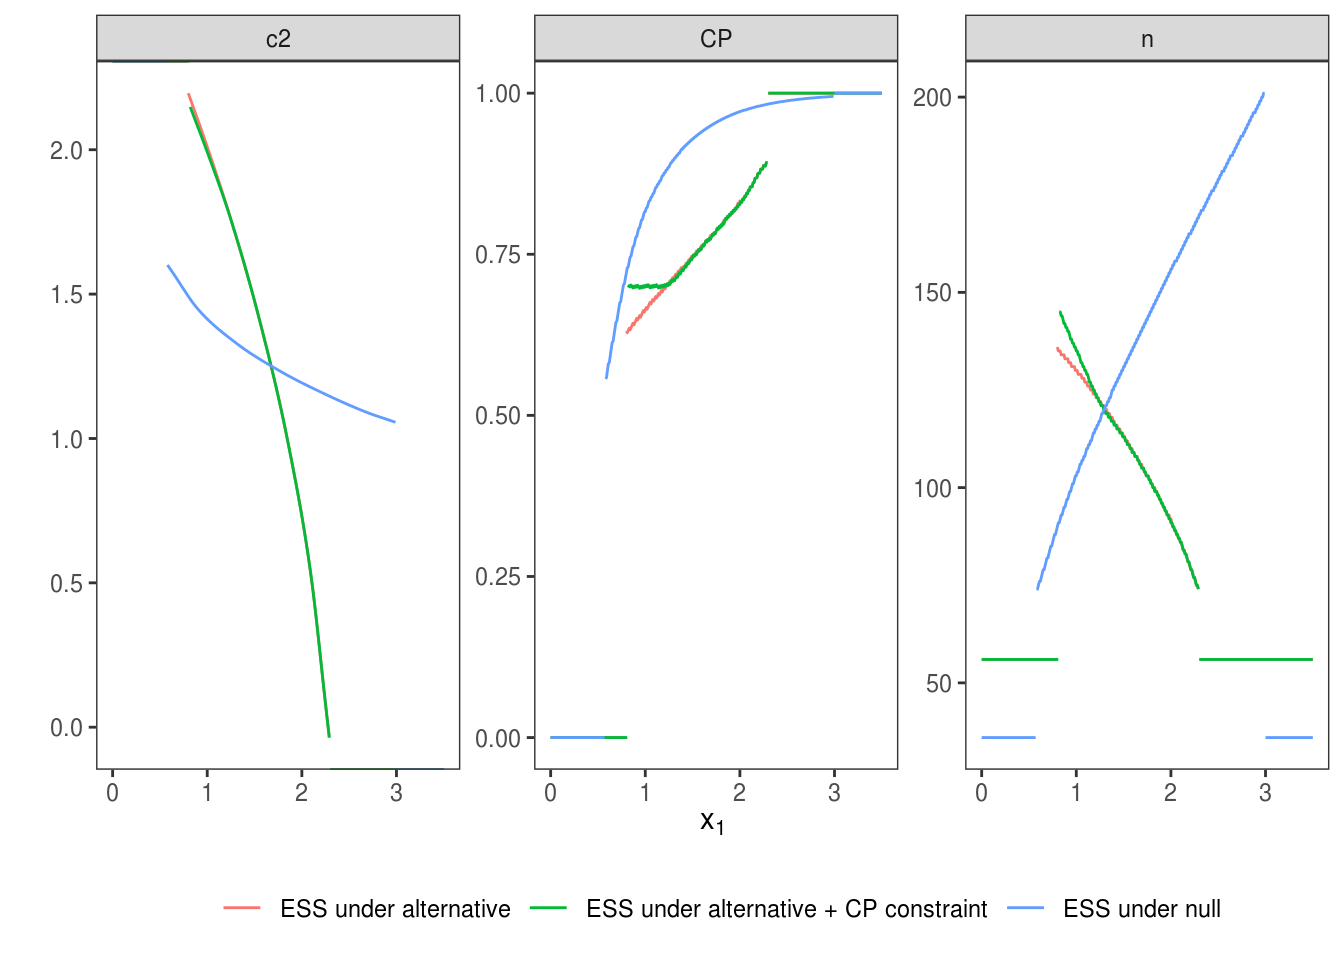
\includegraphics{adoptr-validation-report_files/figure-latex/unnamed-chunk-21-1.pdf}

\hypertarget{scenarioII}{%
\chapter{Scenario II: Large effect, Gaussian prior}\label{scenarioII}}

\hypertarget{details-1}{%
\section{Details}\label{details-1}}

In this scenario, we revisit the case from \protect\hyperlink{scenarioI}{Scenario I}, but
are not assuming a point prior any more.
Instead, a Gaussian prior with mean \(\vartheta = 0.4\) and
variance \(\tau^2 = 0.2^2\) on the effect size is assumed, i.e.
\(\delta \sim \mathcal{N} (0.4, 0.2^2)\).

In order to fulfill regulartory considerations, the type one error rate
is still protected under the point prior \(\delta = 0\) at the level
of significance \(\alpha = 0.025\).

The power constraint, however, needs to be modified.
It is not senseful to compute the power as rejection probability under
the full prior, because effect sizes less than a minimal clinically relevant
effect do not show (sufficient) evidence againt the null hypothesis.
Therefore, we assume a minimal clinically relevant effect size
\(\delta = 0.0\) and condition the prior to compute expected power.
In the following, the expected power should be at least \(0.8\).

\begin{Shaded}
\begin{Highlighting}[]
\CommentTok{# data distribution and priors}
\NormalTok{datadist   <-}\StringTok{ }\KeywordTok{Normal}\NormalTok{(}\DataTypeTok{two_armed =} \OtherTok{TRUE}\NormalTok{)}
\NormalTok{H_}\DecValTok{0}\NormalTok{        <-}\StringTok{ }\KeywordTok{PointMassPrior}\NormalTok{(.}\DecValTok{0}\NormalTok{, }\DecValTok{1}\NormalTok{)}
\NormalTok{prior      <-}\StringTok{ }\KeywordTok{ContinuousPrior}\NormalTok{(}\ControlFlowTok{function}\NormalTok{(delta) }\KeywordTok{dnorm}\NormalTok{(delta, }\DataTypeTok{mean =} \FloatTok{.4}\NormalTok{, }\DataTypeTok{sd =} \FloatTok{.2}\NormalTok{),}
                              \DataTypeTok{support =} \KeywordTok{c}\NormalTok{(}\OperatorTok{-}\DecValTok{5}\NormalTok{, }\DecValTok{5}\NormalTok{),}
                              \DataTypeTok{tighten_support =} \OtherTok{TRUE}\NormalTok{)}

\CommentTok{# define constraints on type one error rate and expected power}
\NormalTok{alpha      <-}\StringTok{ }\FloatTok{0.025}
\NormalTok{min_epower <-}\StringTok{ }\FloatTok{0.8}
\NormalTok{toer_cnstr <-}\StringTok{ }\KeywordTok{Power}\NormalTok{(datadist, H_}\DecValTok{0}\NormalTok{) }\OperatorTok{<=}\StringTok{ }\NormalTok{alpha}
\NormalTok{epow_cnstr <-}\StringTok{ }\KeywordTok{Power}\NormalTok{(datadist, }\KeywordTok{condition}\NormalTok{(prior, }\KeywordTok{c}\NormalTok{(}\FloatTok{0.0}\NormalTok{, prior}\OperatorTok{@}\NormalTok{support[}\DecValTok{2}\NormalTok{]))) }\OperatorTok{>=}\StringTok{ }\NormalTok{min_epower}
\end{Highlighting}
\end{Shaded}

\hypertarget{variantII_1}{%
\section{Variant II-1: Minimizing Expected Sample Size under Point Prior}\label{variantII_1}}

\hypertarget{objective-3}{%
\subsection{Objective}\label{objective-3}}

Expected sample size under the full prior is minimized, i.e.,
\(\boldsymbol{E}\big[n(\mathcal{D})\big]\).

\begin{Shaded}
\begin{Highlighting}[]
\NormalTok{ess <-}\StringTok{ }\KeywordTok{ExpectedSampleSize}\NormalTok{(datadist, prior)}
\end{Highlighting}
\end{Shaded}

\hypertarget{constraints-3}{%
\subsection{Constraints}\label{constraints-3}}

No additional constraints are considered in this variant.

\hypertarget{initial-design-2}{%
\subsection{Initial Design}\label{initial-design-2}}

For this example, the optimal one-stage, group-sequential, and generic
two-stage designs are computed.
While the initial design for the one-stage case is determined heuristically,
both the group sequential and the generic two-stage designs are
optimized starting from the a group-sequential design that is computed by
the \texttt{rpact} package to fulfill the type one error rate constraint and
that fulfills the power constraint at an effect size of \(\delta = 0.3\).

\begin{Shaded}
\begin{Highlighting}[]
\NormalTok{order <-}\StringTok{ }\NormalTok{5L}
\CommentTok{# data frame of initial designs }
\NormalTok{tbl_designs <-}\StringTok{ }\KeywordTok{tibble}\NormalTok{(}
    \DataTypeTok{type    =} \KeywordTok{c}\NormalTok{(}\StringTok{"one-stage"}\NormalTok{, }\StringTok{"group-sequential"}\NormalTok{, }\StringTok{"two-stage"}\NormalTok{),}
    \DataTypeTok{initial =} \KeywordTok{list}\NormalTok{(}
        \KeywordTok{OneStageDesign}\NormalTok{(}\DecValTok{250}\NormalTok{, }\FloatTok{2.0}\NormalTok{),}
        \KeywordTok{rpact_design}\NormalTok{(}\FloatTok{0.3}\NormalTok{, }\FloatTok{0.025}\NormalTok{, }\FloatTok{0.8}\NormalTok{, }\OtherTok{TRUE}\NormalTok{, order),}
        \KeywordTok{TwoStageDesign}\NormalTok{(}\KeywordTok{rpact_design}\NormalTok{(}\FloatTok{0.3}\NormalTok{, }\FloatTok{0.025}\NormalTok{, }\FloatTok{0.8}\NormalTok{, }\OtherTok{TRUE}\NormalTok{, order))) )}
\end{Highlighting}
\end{Shaded}

The order of integration is set to 5.

\hypertarget{optimization-3}{%
\subsection{Optimization}\label{optimization-3}}

For all these three initial designs, the resulting optimal designs are
computed.

\begin{Shaded}
\begin{Highlighting}[]
\NormalTok{tbl_designs <-}\StringTok{ }\NormalTok{tbl_designs }\OperatorTok\StringTok{ }
\StringTok{    }\KeywordTok{mutate}\NormalTok{(}
       \DataTypeTok{optimal =}\NormalTok{ purrr}\OperatorTok{::}\KeywordTok{map}\NormalTok{(initial, }\OperatorTok{~}\KeywordTok{minimize}\NormalTok{(}
         
\NormalTok{          ess,}
          \KeywordTok{subject_to}\NormalTok{(}
\NormalTok{              toer_cnstr,}
\NormalTok{              epow_cnstr}
\NormalTok{          ),}
          
          \DataTypeTok{initial_design =}\NormalTok{ ., }
          \DataTypeTok{opts           =}\NormalTok{ opts)) )}
\end{Highlighting}
\end{Shaded}

\hypertarget{test-cases-3}{%
\subsection{Test Cases}\label{test-cases-3}}

Firstly, it is checked that the maximum number of iterations was not reached
in all these cases.

\begin{Shaded}
\begin{Highlighting}[]
\NormalTok{tbl_designs }\OperatorTok\StringTok{ }
\StringTok{  }\KeywordTok{transmute}\NormalTok{(}
\NormalTok{      type, }
      \DataTypeTok{iterations =}\NormalTok{ purrr}\OperatorTok{::}\KeywordTok{map_int}\NormalTok{(tbl_designs}\OperatorTok{$}\NormalTok{optimal, }
                                  \OperatorTok{~}\NormalTok{.}\OperatorTok{$}\NormalTok{nloptr_return}\OperatorTok{$}\NormalTok{iterations) ) }\OperatorTok
\StringTok{  }\NormalTok{\{}\KeywordTok{print}\NormalTok{(.); .\} }\OperatorTok\StringTok{ }
\StringTok{  }\NormalTok{\{testthat}\OperatorTok{::}\KeywordTok{expect_true}\NormalTok{(}\KeywordTok{all}\NormalTok{(.}\OperatorTok{$}\NormalTok{iterations }\OperatorTok{<}\StringTok{ }\NormalTok{opts}\OperatorTok{$}\NormalTok{maxeval))\}}
\end{Highlighting}
\end{Shaded}

\begin{verbatim}
## # A tibble: 3 x 2
##   type             iterations
##   <chr>                 <int>
## 1 one-stage                21
## 2 group-sequential        670
## 3 two-stage              1928
\end{verbatim}

Since type one error rate is defined under the point effect size \(\delta=0\),
the type one error rate constraint can be tested for all three optimal designs.

\begin{Shaded}
\begin{Highlighting}[]
\NormalTok{tbl_designs }\OperatorTok\StringTok{ }
\StringTok{  }\KeywordTok{transmute}\NormalTok{(}
\NormalTok{      type, }
      \DataTypeTok{toer =}\NormalTok{ purrr}\OperatorTok{::}\KeywordTok{map}\NormalTok{(tbl_designs}\OperatorTok{$}\NormalTok{optimal, }
                        \OperatorTok{~}\KeywordTok{sim_pr_reject}\NormalTok{(.[[}\DecValTok{1}\NormalTok{]], }\FloatTok{.0}\NormalTok{, datadist)}\OperatorTok{$}\NormalTok{prob) ) }\OperatorTok\StringTok{ }
\StringTok{  }\KeywordTok{unnest}\NormalTok{() }\OperatorTok\StringTok{ }
\StringTok{  }\NormalTok{\{}\KeywordTok{print}\NormalTok{(.); .\} }\OperatorTok\StringTok{ }\NormalTok{\{}
\NormalTok{  testthat}\OperatorTok{::}\KeywordTok{expect_true}\NormalTok{(}\KeywordTok{all}\NormalTok{(.}\OperatorTok{$}\NormalTok{toer }\OperatorTok{<=}\StringTok{ }\NormalTok{alpha }\OperatorTok{*}\StringTok{ }\NormalTok{(}\DecValTok{1} \OperatorTok{+}\StringTok{ }\NormalTok{tol))) \}}
\end{Highlighting}
\end{Shaded}

\begin{verbatim}
## # A tibble: 3 x 2
##   type               toer
##   <chr>             <dbl>
## 1 one-stage        0.0251
## 2 group-sequential 0.0249
## 3 two-stage        0.0250
\end{verbatim}

Since the optimal two-stage design is more flexible than the optimal
group-sequential design (constant \(n_2\) function) and this is
more flexible than the optimal one-stage design (no second stage),
the expected sample sizes under the prior should be ordered in the opposite way.
Additionally, expected sample sizes under the null hypothesis
is computed both via \texttt{evaluate()} and simulation-based.

\begin{Shaded}
\begin{Highlighting}[]
\NormalTok{essh0 <-}\StringTok{ }\KeywordTok{ExpectedSampleSize}\NormalTok{(datadist, H_}\DecValTok{0}\NormalTok{)}

\NormalTok{tbl_designs }\OperatorTok\StringTok{ }
\StringTok{    }\KeywordTok{mutate}\NormalTok{(}
        \DataTypeTok{ess       =} \KeywordTok{map_dbl}\NormalTok{(optimal,}
                            \OperatorTok{~}\KeywordTok{evaluate}\NormalTok{(ess, .}\OperatorTok{$}\NormalTok{design) ),}
        \DataTypeTok{essh0     =} \KeywordTok{map_dbl}\NormalTok{(optimal,}
                            \OperatorTok{~}\KeywordTok{evaluate}\NormalTok{(essh0, .}\OperatorTok{$}\NormalTok{design) ),}
        \DataTypeTok{essh0_sim =} \KeywordTok{map_dbl}\NormalTok{(optimal,}
                            \OperatorTok{~}\KeywordTok{sim_n}\NormalTok{(.}\OperatorTok{$}\NormalTok{design, }\FloatTok{.0}\NormalTok{, datadist)}\OperatorTok{$}\NormalTok{n ) ) }\OperatorTok\StringTok{ }
\StringTok{    }\NormalTok{\{}\KeywordTok{print}\NormalTok{(.); .\} }\OperatorTok\StringTok{ }\NormalTok{\{}
    \CommentTok{# sim/evaluate same under null?}
\NormalTok{    testthat}\OperatorTok{::}\KeywordTok{expect_equal}\NormalTok{(.}\OperatorTok{$}\NormalTok{essh0, .}\OperatorTok{$}\NormalTok{essh0_sim, }
                           \DataTypeTok{tolerance =}\NormalTok{ tol_n,}
                           \DataTypeTok{scale =} \DecValTok{1}\NormalTok{)}
    \CommentTok{# monotonicity with respect to degrees of freedom}
\NormalTok{    testthat}\OperatorTok{::}\KeywordTok{expect_true}\NormalTok{(}\KeywordTok{all}\NormalTok{(}\KeywordTok{diff}\NormalTok{(.}\OperatorTok{$}\NormalTok{ess) }\OperatorTok{<}\StringTok{ }\DecValTok{0}\NormalTok{)) \}}
\end{Highlighting}
\end{Shaded}

\begin{verbatim}
## # A tibble: 3 x 6
##   type             initial    optimal      ess essh0 essh0_sim
##   <chr>            <list>     <list>     <dbl> <dbl>     <dbl>
## 1 one-stage        <OnStgDsg> <list [3]>  165   165       165 
## 2 group-sequential <GrpSqntD> <list [3]>  115.  110.      110.
## 3 two-stage        <TwStgDsg> <list [3]>  113.  114.      114.
\end{verbatim}

\hypertarget{variantII_2}{%
\section{Variant II-2: Minimizing Expected Sample Size under Null Hypothesis}\label{variantII_2}}

\hypertarget{objective-4}{%
\subsection{Objective}\label{objective-4}}

Expected sample size conditioned on negative effect sizes is minimized, i.e.,

\begin{Shaded}
\begin{Highlighting}[]
\NormalTok{ess_}\DecValTok{0}\NormalTok{ <-}\StringTok{ }\KeywordTok{ExpectedSampleSize}\NormalTok{(datadist, }\KeywordTok{condition}\NormalTok{(prior, }\KeywordTok{c}\NormalTok{(}\KeywordTok{bounds}\NormalTok{(prior)[}\DecValTok{1}\NormalTok{], }\DecValTok{0}\NormalTok{)))}
\end{Highlighting}
\end{Shaded}

\hypertarget{constraints-4}{%
\subsection{Constraints}\label{constraints-4}}

No additional constraints besides type one error rate and expected power
are considered in this variant.

\hypertarget{initial-design-3}{%
\subsection{Initial Design}\label{initial-design-3}}

As in \protect\hyperlink{variantI_2}{Variant I.2} another initial design is more appropriate
for optimization under the null hypothesis.
In this situation, one may expect a different (increasing) sample size function,
and thus also a different shape of the \(c_2\) function.
Therefore, the \texttt{rpact} initial design is a suboptimal starting point.
Instead, we start with a constant \(c_2\) function by heuristically
setting it to \(2\) on the continuation area.

\begin{Shaded}
\begin{Highlighting}[]
\NormalTok{init_design_h0 <-}\StringTok{ }\NormalTok{tbl_designs }\OperatorTok\StringTok{ }
\StringTok{    }\KeywordTok{filter}\NormalTok{(type }\OperatorTok{==}\StringTok{ "two-stage"}\NormalTok{) }\OperatorTok\StringTok{ }
\StringTok{    }\KeywordTok{pull}\NormalTok{(initial) }\OperatorTok\StringTok{ }
\StringTok{    }\NormalTok{.[[}\DecValTok{1}\NormalTok{]]}
\NormalTok{init_design_h0}\OperatorTok{@}\NormalTok{c2_pivots <-}\StringTok{ }\KeywordTok{rep}\NormalTok{(}\DecValTok{2}\NormalTok{, order)}
\end{Highlighting}
\end{Shaded}

\hypertarget{optimization-4}{%
\subsection{Optimization}\label{optimization-4}}

The optimal two-stage design is computed.

\begin{Shaded}
\begin{Highlighting}[]
\NormalTok{opt_neg <-}\StringTok{ }\KeywordTok{minimize}\NormalTok{(}
  
\NormalTok{        ess_}\DecValTok{0}\NormalTok{,}
        
        \KeywordTok{subject_to}\NormalTok{(}
          
\NormalTok{            toer_cnstr,}
\NormalTok{            epow_cnstr}
\NormalTok{        ),}
        
        \DataTypeTok{initial_design =}\NormalTok{ init_design_h0,}
        \DataTypeTok{opts =}\NormalTok{ opts}
\NormalTok{)}
\end{Highlighting}
\end{Shaded}

\hypertarget{test-cases-4}{%
\subsection{Test Cases}\label{test-cases-4}}

First of all, check if the optimization algorithm converged.
To avoid improper solutions, it is first verified that the maximum
number of iterations was not exceeded in any of the three cases.

\begin{Shaded}
\begin{Highlighting}[]
\NormalTok{testthat}\OperatorTok{::}\KeywordTok{expect_true}\NormalTok{(opt_neg}\OperatorTok{$}\NormalTok{nloptr_return}\OperatorTok{$}\NormalTok{iterations }\OperatorTok{<}\StringTok{ }\NormalTok{opts}\OperatorTok{$}\NormalTok{maxeval)}
\KeywordTok{print}\NormalTok{(opt_neg}\OperatorTok{$}\NormalTok{nloptr_return}\OperatorTok{$}\NormalTok{iterations)}
\end{Highlighting}
\end{Shaded}

\begin{verbatim}
## [1] 1025
\end{verbatim}

Again, the type one error rate under the point null hypothesis \(\delta = 0\)
can be tested by simulation.

\begin{Shaded}
\begin{Highlighting}[]
\NormalTok{tbl_toer <-}\StringTok{ }\KeywordTok{tibble}\NormalTok{(}
  \DataTypeTok{toer     =} \KeywordTok{evaluate}\NormalTok{(}\KeywordTok{Power}\NormalTok{(datadist, H_}\DecValTok{0}\NormalTok{), opt_neg}\OperatorTok{$}\NormalTok{design),}
  \DataTypeTok{toer_sim =} \KeywordTok{sim_pr_reject}\NormalTok{(opt_neg}\OperatorTok{$}\NormalTok{design, }\FloatTok{.0}\NormalTok{, datadist)}\OperatorTok{$}\NormalTok{prob}
\NormalTok{)}

\KeywordTok{print}\NormalTok{(tbl_toer)}
\end{Highlighting}
\end{Shaded}

\begin{verbatim}
## # A tibble: 1 x 2
##     toer toer_sim
##    <dbl>    <dbl>
## 1 0.0250   0.0250
\end{verbatim}

\begin{Shaded}
\begin{Highlighting}[]
\NormalTok{testthat}\OperatorTok{::}\KeywordTok{expect_true}\NormalTok{(tbl_toer}\OperatorTok{$}\NormalTok{toer }\OperatorTok{<=}\StringTok{ }\NormalTok{alpha }\OperatorTok{*}\StringTok{ }\NormalTok{(}\DecValTok{1} \OperatorTok{+}\StringTok{ }\NormalTok{tol))}
\NormalTok{testthat}\OperatorTok{::}\KeywordTok{expect_true}\NormalTok{(tbl_toer}\OperatorTok{$}\NormalTok{toer_sim }\OperatorTok{<=}\StringTok{ }\NormalTok{alpha }\OperatorTok{*}\StringTok{ }\NormalTok{(}\DecValTok{1} \OperatorTok{+}\StringTok{ }\NormalTok{tol))}
\end{Highlighting}
\end{Shaded}

Furthermore, the expected sample size under the prior conditioned on negative
effect sizes (\(\delta \leq 0\)) should be lower for the optimal design derived
in this variant than for the optimal design from \protect\hyperlink{variantII_1}{Variant II.1}
where expected sample size under the full prior was minimized.

\begin{Shaded}
\begin{Highlighting}[]
\NormalTok{testthat}\OperatorTok{::}\KeywordTok{expect_lte}\NormalTok{(}
    \KeywordTok{evaluate}\NormalTok{(ess_}\DecValTok{0}\NormalTok{, opt_neg}\OperatorTok{$}\NormalTok{design),}
    \KeywordTok{evaluate}\NormalTok{(}
\NormalTok{        ess_}\DecValTok{0}\NormalTok{, }
\NormalTok{        tbl_designs }\OperatorTok\StringTok{ }
\StringTok{            }\KeywordTok{filter}\NormalTok{(type }\OperatorTok{==}\StringTok{ "two-stage"}\NormalTok{) }\OperatorTok\StringTok{ }
\StringTok{            }\KeywordTok{pull}\NormalTok{(optimal) }\OperatorTok\StringTok{ }
\StringTok{            }\NormalTok{.[[}\DecValTok{1}\NormalTok{]] }\OperatorTok\StringTok{ }
\StringTok{            }\NormalTok{.}\OperatorTok{$}\NormalTok{design )}
\NormalTok{)}
\end{Highlighting}
\end{Shaded}

\hypertarget{variantII_3}{%
\section{Variant II-3: Conditional Power Constraint}\label{variantII_3}}

\hypertarget{objective-5}{%
\subsection{Objective}\label{objective-5}}

As in \protect\hyperlink{variantII_1}{Variant II-1}, expected sample size under the full prior
is minimized.

\hypertarget{constraints-5}{%
\subsection{Constraints}\label{constraints-5}}

In addition to the constraints on type one error rate and expected power,
a constraint on conditional power to be larger than \(0.7\) is included.

\begin{Shaded}
\begin{Highlighting}[]
\NormalTok{cp <-}\StringTok{ }\KeywordTok{ConditionalPower}\NormalTok{(datadist, }\KeywordTok{condition}\NormalTok{(prior, }\KeywordTok{c}\NormalTok{(}\DecValTok{0}\NormalTok{, prior}\OperatorTok{@}\NormalTok{support[}\DecValTok{2}\NormalTok{])))}

\NormalTok{cp_cnstr <-}\StringTok{ }\NormalTok{cp }\OperatorTok{>=}\StringTok{ }\FloatTok{0.7}
\end{Highlighting}
\end{Shaded}

\hypertarget{initial-design-4}{%
\subsection{Initial Design}\label{initial-design-4}}

The previous initial design can still be applied.

\hypertarget{optimization-5}{%
\subsection{Optimization}\label{optimization-5}}

The optimal two-stage design is computed.

\begin{Shaded}
\begin{Highlighting}[]
\NormalTok{opt_cp <-}\StringTok{ }\KeywordTok{minimize}\NormalTok{(}
\NormalTok{        ess,}
        \KeywordTok{subject_to}\NormalTok{(}
\NormalTok{            toer_cnstr,}
\NormalTok{            epow_cnstr,}
\NormalTok{            cp_cnstr}
\NormalTok{        ),}
        \DataTypeTok{initial_design =}\NormalTok{ tbl_designs}\OperatorTok{$}\NormalTok{initial[[}\DecValTok{3}\NormalTok{]],}
        \DataTypeTok{opts =}\NormalTok{ opts}
\NormalTok{)}
\end{Highlighting}
\end{Shaded}

\hypertarget{test-cases-5}{%
\subsection{Test Cases}\label{test-cases-5}}

We start checking whether the maximum number of iterations was not reached.

\begin{Shaded}
\begin{Highlighting}[]
\KeywordTok{print}\NormalTok{(opt_cp}\OperatorTok{$}\NormalTok{nloptr_return}\OperatorTok{$}\NormalTok{iterations)}
\end{Highlighting}
\end{Shaded}

\begin{verbatim}
## [1] 2154
\end{verbatim}

\begin{Shaded}
\begin{Highlighting}[]
\NormalTok{testthat}\OperatorTok{::}\KeywordTok{expect_true}\NormalTok{(opt_cp}\OperatorTok{$}\NormalTok{nloptr_return}\OperatorTok{$}\NormalTok{iterations }\OperatorTok{<}\StringTok{ }\NormalTok{opts}\OperatorTok{$}\NormalTok{maxeval)}
\end{Highlighting}
\end{Shaded}

The type one error rate is tested via simulation and compared
to the value obtained by \texttt{evaluate()}.

\begin{Shaded}
\begin{Highlighting}[]
\NormalTok{tbl_toer <-}\StringTok{ }\KeywordTok{tibble}\NormalTok{(}
  \DataTypeTok{toer     =} \KeywordTok{evaluate}\NormalTok{(}\KeywordTok{Power}\NormalTok{(datadist, H_}\DecValTok{0}\NormalTok{), opt_cp}\OperatorTok{$}\NormalTok{design),}
  \DataTypeTok{toer_sim =} \KeywordTok{sim_pr_reject}\NormalTok{(opt_cp}\OperatorTok{$}\NormalTok{design, }\FloatTok{.0}\NormalTok{, datadist)}\OperatorTok{$}\NormalTok{prob}
\NormalTok{)}

\KeywordTok{print}\NormalTok{(tbl_toer)}
\end{Highlighting}
\end{Shaded}

\begin{verbatim}
## # A tibble: 1 x 2
##     toer toer_sim
##    <dbl>    <dbl>
## 1 0.0250   0.0250
\end{verbatim}

\begin{Shaded}
\begin{Highlighting}[]
\NormalTok{testthat}\OperatorTok{::}\KeywordTok{expect_true}\NormalTok{(tbl_toer}\OperatorTok{$}\NormalTok{toer }\OperatorTok{<=}\StringTok{ }\NormalTok{alpha }\OperatorTok{*}\StringTok{ }\NormalTok{(}\DecValTok{1} \OperatorTok{+}\StringTok{ }\NormalTok{tol))}
\NormalTok{testthat}\OperatorTok{::}\KeywordTok{expect_true}\NormalTok{(tbl_toer}\OperatorTok{$}\NormalTok{toer_sim }\OperatorTok{<=}\StringTok{ }\NormalTok{alpha }\OperatorTok{*}\StringTok{ }\NormalTok{(}\DecValTok{1} \OperatorTok{+}\StringTok{ }\NormalTok{tol))}
\end{Highlighting}
\end{Shaded}

The conditional power is evaluated via numerical integration on several points
inside the continuation region and it is tested whether the constraint is
fulfilled on all these points.

\begin{Shaded}
\begin{Highlighting}[]
\KeywordTok{tibble}\NormalTok{(}
    \DataTypeTok{x1 =} \KeywordTok{seq}\NormalTok{(opt_cp}\OperatorTok{$}\NormalTok{design}\OperatorTok{@}\NormalTok{c1f, opt_cp}\OperatorTok{$}\NormalTok{design}\OperatorTok{@}\NormalTok{c1e, }\DataTypeTok{length.out =} \DecValTok{25}\NormalTok{),}
    \DataTypeTok{cp =} \KeywordTok{map_dbl}\NormalTok{(x1, }\OperatorTok{~}\KeywordTok{evaluate}\NormalTok{(cp, opt_cp}\OperatorTok{$}\NormalTok{design, .)) ) }\OperatorTok\StringTok{ }
\StringTok{  }\NormalTok{\{}\KeywordTok{print}\NormalTok{(.); .\} }\OperatorTok\StringTok{ }\NormalTok{\{}
\NormalTok{      testthat}\OperatorTok{::}\KeywordTok{expect_true}\NormalTok{(}\KeywordTok{all}\NormalTok{(.}\OperatorTok{$}\NormalTok{cp }\OperatorTok{>=}\StringTok{ }\FloatTok{0.7} \OperatorTok{*}\StringTok{ }\NormalTok{(}\DecValTok{1} \OperatorTok{-}\StringTok{ }\NormalTok{tol))) \}}
\end{Highlighting}
\end{Shaded}

\begin{verbatim}
## # A tibble: 25 x 2
##       x1    cp
##    <dbl> <dbl>
##  1 0.718 0.696
##  2 0.787 0.700
##  3 0.855 0.702
##  4 0.924 0.700
##  5 0.993 0.699
##  6 1.06  0.698
##  7 1.13  0.702
##  8 1.20  0.708
##  9 1.27  0.716
## 10 1.34  0.725
## # ... with 15 more rows
\end{verbatim}

Due to the additional constraint in comparison to \protect\hyperlink{variantII_1}{Variant II.1},
Variant II.3 should show a larger expected sample size under the prior than
Variant II.1

\begin{Shaded}
\begin{Highlighting}[]
\NormalTok{testthat}\OperatorTok{::}\KeywordTok{expect_gte}\NormalTok{(}
    \KeywordTok{evaluate}\NormalTok{(ess, opt_cp}\OperatorTok{$}\NormalTok{design),}
    \KeywordTok{evaluate}\NormalTok{(}
\NormalTok{        ess, }
\NormalTok{        tbl_designs }\OperatorTok\StringTok{ }
\StringTok{            }\KeywordTok{filter}\NormalTok{(type }\OperatorTok{==}\StringTok{ "two-stage"}\NormalTok{) }\OperatorTok\StringTok{ }
\StringTok{            }\KeywordTok{pull}\NormalTok{(optimal) }\OperatorTok\StringTok{ }
\StringTok{            }\NormalTok{.[[}\DecValTok{1}\NormalTok{]] }\OperatorTok\StringTok{ }
\StringTok{            }\NormalTok{.}\OperatorTok{$}\NormalTok{design )}
\NormalTok{)}
\end{Highlighting}
\end{Shaded}

\hypertarget{plot-two-stage-designs-1}{%
\section{Plot Two-Stage Designs}\label{plot-two-stage-designs-1}}

The optimal two-stage designs stemming from the different variants
are plotted together.

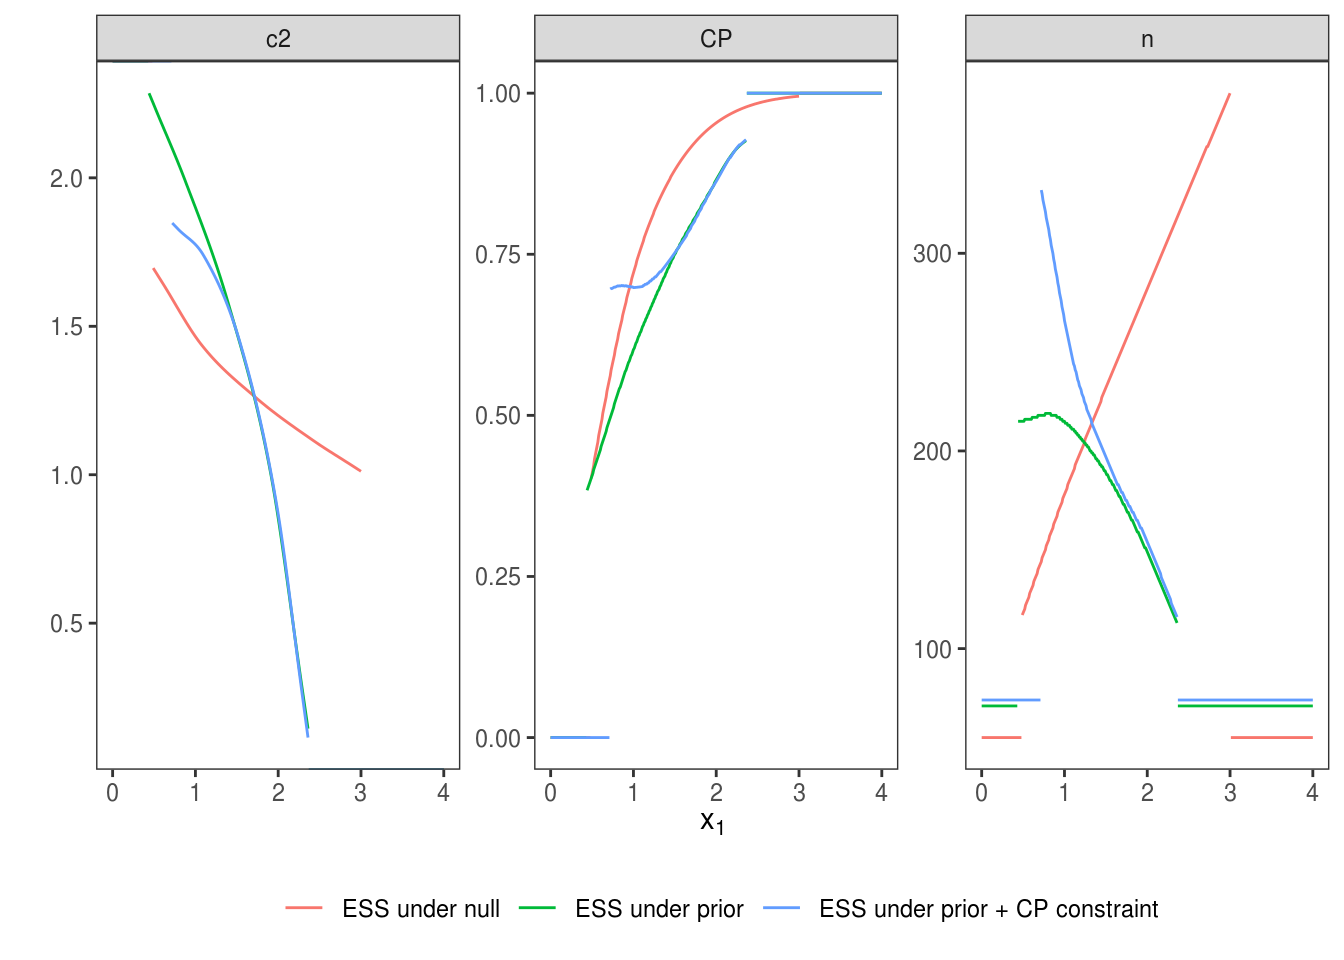
\includegraphics{adoptr-validation-report_files/figure-latex/unnamed-chunk-41-1.pdf}

\hypertarget{scenarioIII}{%
\chapter{Scenario III: large effect, uniform prior}\label{scenarioIII}}

\hypertarget{details-2}{%
\section{Details}\label{details-2}}

This scenario covers a similar setting as \protect\hyperlink{scenarioI}{Scenario I}.
The purpose is to asses whether placing uniform priors with decreasing
width of support centered at the \(\delta=0.4\) leads to a sequence of
optimal designs which converges towards the solution in \protect\hyperlink{variantI.1}{variant I-1}.

The trial is still considered to be two-armed with normally distribtuted outcomes
and the type one error rate under the null hypothesis
\(\mathcal{H}_0:\delta \leq 0\) is to be protected at \(\alpha = 0.025\).

\begin{Shaded}
\begin{Highlighting}[]
\NormalTok{datadist   <-}\StringTok{ }\KeywordTok{Normal}\NormalTok{(}\DataTypeTok{two_armed =} \OtherTok{TRUE}\NormalTok{)}
\NormalTok{H_}\DecValTok{0}\NormalTok{        <-}\StringTok{ }\KeywordTok{PointMassPrior}\NormalTok{(.}\DecValTok{0}\NormalTok{, }\DecValTok{1}\NormalTok{)}
\NormalTok{alpha      <-}\StringTok{ }\FloatTok{0.025}
\NormalTok{toer_cnstr <-}\StringTok{ }\KeywordTok{Power}\NormalTok{(datadist, H_}\DecValTok{0}\NormalTok{) }\OperatorTok{<=}\StringTok{ }\NormalTok{alpha}
\end{Highlighting}
\end{Shaded}

In this scenario we consider a sequence of uniform distributions
\(\delta\sim\operatorname{Unif}(0.4 - \Delta_i, 0.4 + \Delta_i)\)
around \(0.4\) with \(\Delta_i=(3 - i)/10\) for \(i=0\ldots 3\).
I.e., for \(\Delta_3=0\) reduces to \texttt{PointMassPrior} on \(\delta=0.4\).

\begin{Shaded}
\begin{Highlighting}[]
\NormalTok{prior <-}\StringTok{ }\ControlFlowTok{function}\NormalTok{(delta) \{}
    \ControlFlowTok{if}\NormalTok{ (delta }\OperatorTok{==}\StringTok{ }\DecValTok{0}\NormalTok{)}
        \KeywordTok{return}\NormalTok{(}\KeywordTok{PointMassPrior}\NormalTok{(.}\DecValTok{4}\NormalTok{, }\FloatTok{1.0}\NormalTok{))}
\NormalTok{    a <-}\StringTok{ }\FloatTok{.4} \OperatorTok{-}\StringTok{ }\NormalTok{delta; b <-}\StringTok{ }\FloatTok{.4} \OperatorTok{+}\StringTok{ }\NormalTok{delta}
    \KeywordTok{ContinuousPrior}\NormalTok{(}\ControlFlowTok{function}\NormalTok{(x) }\KeywordTok{dunif}\NormalTok{(x, a, b), }\DataTypeTok{support =} \KeywordTok{c}\NormalTok{(a, b))}
\NormalTok{\}}
\end{Highlighting}
\end{Shaded}

Across all variants in this scenario, the expected power under the respective
prior conditioned on \(\delta > 0\) must be at least \(0.8\).
I.e., throughout this scenario, we always use the following constraint on
expected power.

\begin{Shaded}
\begin{Highlighting}[]
\NormalTok{ep_cnstr <-}\StringTok{ }\ControlFlowTok{function}\NormalTok{(delta) \{}
\NormalTok{    prior     <-}\StringTok{ }\KeywordTok{prior}\NormalTok{(delta)}
\NormalTok{    cnd_prior <-}\StringTok{ }\KeywordTok{condition}\NormalTok{(prior, }\KeywordTok{c}\NormalTok{(}\DecValTok{0}\NormalTok{, }\KeywordTok{bounds}\NormalTok{(prior)[}\DecValTok{2}\NormalTok{]))}
    \KeywordTok{return}\NormalTok{( }\KeywordTok{Power}\NormalTok{(datadist, cnd_prior) }\OperatorTok{>=}\StringTok{ }\FloatTok{0.8}\NormalTok{ )}
\NormalTok{\}}
\end{Highlighting}
\end{Shaded}

\hypertarget{variantIII_1}{%
\section{Variant III.1: Convergence under prior concentration}\label{variantIII_1}}

The goal of this variant is to make sure that the optimal solution
converges as the prior is more and more concentrated at a point mass.

\hypertarget{objective-6}{%
\subsection{Objective}\label{objective-6}}

Expected sample size under the respective prior is minimized, i.e.,
\(\boldsymbol{E}\big[n(\mathcal{D})\big]\).

\begin{Shaded}
\begin{Highlighting}[]
\NormalTok{objective <-}\StringTok{ }\ControlFlowTok{function}\NormalTok{(delta) \{}
    \KeywordTok{ExpectedSampleSize}\NormalTok{(datadist, }\KeywordTok{prior}\NormalTok{(delta))}
\NormalTok{\}}
\end{Highlighting}
\end{Shaded}

\hypertarget{constraints-6}{%
\subsection{Constraints}\label{constraints-6}}

The constraints have already been described under details.

\hypertarget{optimization-problem}{%
\subsection{Optimization problem}\label{optimization-problem}}

The optimization problem depending on \(\Delta_i\) is defined below.
The default optimization parameters, 5 pivot points, and a fixed initial design
are used.
The initial design is chosen such that the error constraints are
fulfilled. Early stopping for futility is applied if the effect shows
in the opponent direction to the alternative, i.e. \(c_1^f=0\).
\(c_2\) is chosen close to and \(c_1^e\) a little larger than the \(1-\alpha\)-quantile
of the standard normal distribution. The sample sizes are selected
to fulfill the error constraints.

\begin{Shaded}
\begin{Highlighting}[]
\NormalTok{init <-}\StringTok{ }\KeywordTok{TwoStageDesign}\NormalTok{(}
    \DataTypeTok{n1    =} \DecValTok{150}\NormalTok{,}
    \DataTypeTok{c1f   =} \DecValTok{0}\NormalTok{,}
    \DataTypeTok{c1e   =} \FloatTok{2.3}\NormalTok{,}
    \DataTypeTok{n2    =} \FloatTok{125.0}\NormalTok{,}
    \DataTypeTok{c2    =} \FloatTok{2.0}\NormalTok{,}
    \DataTypeTok{order =} \DecValTok{5}
\NormalTok{)}

\NormalTok{optimal_design <-}\StringTok{ }\ControlFlowTok{function}\NormalTok{(delta) \{}
    \KeywordTok{minimize}\NormalTok{(}
        \KeywordTok{objective}\NormalTok{(delta),}
        \KeywordTok{subject_to}\NormalTok{(}
\NormalTok{            toer_cnstr,}
            \KeywordTok{ep_cnstr}\NormalTok{(delta)}
\NormalTok{        ),}
        \DataTypeTok{initial_design =}\NormalTok{ init}
\NormalTok{    )}
\NormalTok{\}}

\CommentTok{# compute the sequence of optimal designs}
\NormalTok{deltas  <-}\StringTok{ }\DecValTok{3}\OperatorTok{:}\DecValTok{0}\OperatorTok{/}\DecValTok{10}
\NormalTok{results <-}\StringTok{ }\KeywordTok{lapply}\NormalTok{(deltas, optimal_design)}
\end{Highlighting}
\end{Shaded}

\hypertarget{test-cases-6}{%
\subsection{Test cases}\label{test-cases-6}}

Check that iteration limit was not exceeded in any case.

\begin{Shaded}
\begin{Highlighting}[]
\NormalTok{iters <-}\StringTok{ }\KeywordTok{sapply}\NormalTok{(results, }\ControlFlowTok{function}\NormalTok{(x) x}\OperatorTok{$}\NormalTok{nloptr_return}\OperatorTok{$}\NormalTok{iterations)}
\KeywordTok{print}\NormalTok{(iters)}
\end{Highlighting}
\end{Shaded}

\begin{verbatim}
## [1] 1746 1857 2438 2684
\end{verbatim}

\begin{Shaded}
\begin{Highlighting}[]
\NormalTok{testthat}\OperatorTok{::}\KeywordTok{expect_true}\NormalTok{(}\KeywordTok{all}\NormalTok{(iters }\OperatorTok{<=}\StringTok{ }\NormalTok{opts}\OperatorTok{$}\NormalTok{maxeval))}
\end{Highlighting}
\end{Shaded}

Check type one error rate control by simulation and by calling \texttt{evaluate()}.

\begin{Shaded}
\begin{Highlighting}[]
\NormalTok{df_toer <-}\StringTok{ }\KeywordTok{tibble}\NormalTok{(}
  \DataTypeTok{delta    =}\NormalTok{ deltas,}
  \DataTypeTok{toer     =} \KeywordTok{sapply}\NormalTok{(results, }\ControlFlowTok{function}\NormalTok{(x) }\KeywordTok{evaluate}\NormalTok{(}\KeywordTok{Power}\NormalTok{(datadist, H_}\DecValTok{0}\NormalTok{), x}\OperatorTok{$}\NormalTok{design)),}
  \DataTypeTok{toer_sim =} \KeywordTok{sapply}\NormalTok{(results, }\ControlFlowTok{function}\NormalTok{(x) }\KeywordTok{sim_pr_reject}\NormalTok{(x}\OperatorTok{$}\NormalTok{design, }\FloatTok{.0}\NormalTok{, datadist)}\OperatorTok{$}\NormalTok{prob)}
\NormalTok{)}

\NormalTok{testthat}\OperatorTok{::}\KeywordTok{expect_true}\NormalTok{(}\KeywordTok{all}\NormalTok{(df_toer}\OperatorTok{$}\NormalTok{toer     }\OperatorTok{<=}\StringTok{ }\NormalTok{alpha }\OperatorTok{*}\StringTok{ }\NormalTok{(}\DecValTok{1} \OperatorTok{+}\StringTok{ }\NormalTok{tol)))}
\NormalTok{testthat}\OperatorTok{::}\KeywordTok{expect_true}\NormalTok{(}\KeywordTok{all}\NormalTok{(df_toer}\OperatorTok{$}\NormalTok{toer_sim }\OperatorTok{<=}\StringTok{ }\NormalTok{alpha }\OperatorTok{*}\StringTok{ }\NormalTok{(}\DecValTok{1} \OperatorTok{+}\StringTok{ }\NormalTok{tol)))}

\KeywordTok{print}\NormalTok{(df_toer)}
\end{Highlighting}
\end{Shaded}

\begin{verbatim}
## # A tibble: 4 x 3
##   delta   toer toer_sim
##   <dbl>  <dbl>    <dbl>
## 1   0.3 0.0250   0.0250
## 2   0.2 0.0250   0.0250
## 3   0.1 0.0250   0.0250
## 4   0   0.0250   0.0250
\end{verbatim}

Check that expected sample size decreases with decreasing prior variance.

\begin{Shaded}
\begin{Highlighting}[]
\NormalTok{testthat}\OperatorTok{::}\KeywordTok{expect_gte}\NormalTok{(}
  \KeywordTok{evaluate}\NormalTok{(}\KeywordTok{objective}\NormalTok{(deltas[}\DecValTok{1}\NormalTok{]), results[[}\DecValTok{1}\NormalTok{]]}\OperatorTok{$}\NormalTok{design),}
  \KeywordTok{evaluate}\NormalTok{(}\KeywordTok{objective}\NormalTok{(deltas[}\DecValTok{2}\NormalTok{]), results[[}\DecValTok{2}\NormalTok{]]}\OperatorTok{$}\NormalTok{design)}
\NormalTok{)}

\NormalTok{testthat}\OperatorTok{::}\KeywordTok{expect_gte}\NormalTok{(}
  \KeywordTok{evaluate}\NormalTok{(}\KeywordTok{objective}\NormalTok{(deltas[}\DecValTok{2}\NormalTok{]), results[[}\DecValTok{2}\NormalTok{]]}\OperatorTok{$}\NormalTok{design),}
  \KeywordTok{evaluate}\NormalTok{(}\KeywordTok{objective}\NormalTok{(deltas[}\DecValTok{3}\NormalTok{]), results[[}\DecValTok{3}\NormalTok{]]}\OperatorTok{$}\NormalTok{design)}
\NormalTok{)}

\NormalTok{testthat}\OperatorTok{::}\KeywordTok{expect_gte}\NormalTok{(}
  \KeywordTok{evaluate}\NormalTok{(}\KeywordTok{objective}\NormalTok{(deltas[}\DecValTok{3}\NormalTok{]), results[[}\DecValTok{3}\NormalTok{]]}\OperatorTok{$}\NormalTok{design),}
  \KeywordTok{evaluate}\NormalTok{(}\KeywordTok{objective}\NormalTok{(deltas[}\DecValTok{4}\NormalTok{]), results[[}\DecValTok{4}\NormalTok{]]}\OperatorTok{$}\NormalTok{design)}
\NormalTok{)}
\end{Highlighting}
\end{Shaded}

\hypertarget{plot-designs}{%
\subsection{Plot designs}\label{plot-designs}}

Plot and assess for convergence

\begin{Shaded}
\begin{Highlighting}[]
\NormalTok{z1 <-}\StringTok{ }\KeywordTok{seq}\NormalTok{(}\DecValTok{0}\NormalTok{, }\DecValTok{3}\NormalTok{, }\DataTypeTok{by =} \FloatTok{.01}\NormalTok{)}

\KeywordTok{tibble}\NormalTok{(}
    \DataTypeTok{delta  =}\NormalTok{ deltas, }
    \DataTypeTok{design =} \KeywordTok{lapply}\NormalTok{(results, }\ControlFlowTok{function}\NormalTok{(x) x}\OperatorTok{$}\NormalTok{design)}
\NormalTok{) }\OperatorTok\StringTok{ }
\StringTok{    }\KeywordTok{group_by}\NormalTok{(delta) }\OperatorTok\StringTok{ }
\StringTok{    }\KeywordTok{do}\NormalTok{(}
        \DataTypeTok{z1 =}\NormalTok{ z1,}
        \DataTypeTok{n  =}\NormalTok{ adoptr}\OperatorTok{::}\KeywordTok{n}\NormalTok{(.}\OperatorTok{$}\NormalTok{design[[}\DecValTok{1}\NormalTok{]], z1),}
        \DataTypeTok{c2 =} \KeywordTok{c2}\NormalTok{(.}\OperatorTok{$}\NormalTok{design[[}\DecValTok{1}\NormalTok{]], z1)}
\NormalTok{    ) }\OperatorTok\StringTok{ }
\StringTok{    }\KeywordTok{unnest}\NormalTok{() }\OperatorTok\StringTok{ }
\StringTok{    }\KeywordTok{mutate}\NormalTok{(}
        \DataTypeTok{section =} \KeywordTok{ifelse}\NormalTok{(}
            \KeywordTok{is.finite}\NormalTok{(c2), }
            \StringTok{"continuation"}\NormalTok{, }
            \KeywordTok{ifelse}\NormalTok{(c2 }\OperatorTok{==}\StringTok{ }\OperatorTok{-}\OtherTok{Inf}\NormalTok{, }\StringTok{"efficacy"}\NormalTok{, }\StringTok{"futility"}\NormalTok{)}
\NormalTok{        )}
\NormalTok{    ) }\OperatorTok\StringTok{ }
\StringTok{    }\KeywordTok{gather}\NormalTok{(variable, value, n, c2) }\OperatorTok\StringTok{ }
\StringTok{    }\KeywordTok{ggplot}\NormalTok{(}\KeywordTok{aes}\NormalTok{(z1, value, }\DataTypeTok{color =}\NormalTok{ delta)) }\OperatorTok{+}
\StringTok{        }\KeywordTok{geom_line}\NormalTok{(}\KeywordTok{aes}\NormalTok{(}\DataTypeTok{group =} \KeywordTok{interaction}\NormalTok{(section, delta))) }\OperatorTok{+}\StringTok{ }
\StringTok{        }\KeywordTok{facet_wrap}\NormalTok{(}\OperatorTok{~}\NormalTok{variable, }\DataTypeTok{scales =} \StringTok{"free_y"}\NormalTok{) }\OperatorTok{+}
\StringTok{        }\KeywordTok{theme_bw}\NormalTok{() }\OperatorTok{+}
\StringTok{        }\KeywordTok{scale_color_continuous}\NormalTok{(}\KeywordTok{bquote}\NormalTok{(Delta)) }\OperatorTok{+}
\StringTok{        }\KeywordTok{theme}\NormalTok{(}
            \DataTypeTok{panel.grid =} \KeywordTok{element_blank}\NormalTok{(),}
            \DataTypeTok{legend.position =} \StringTok{"bottom"}
\NormalTok{        )}
\end{Highlighting}
\end{Shaded}

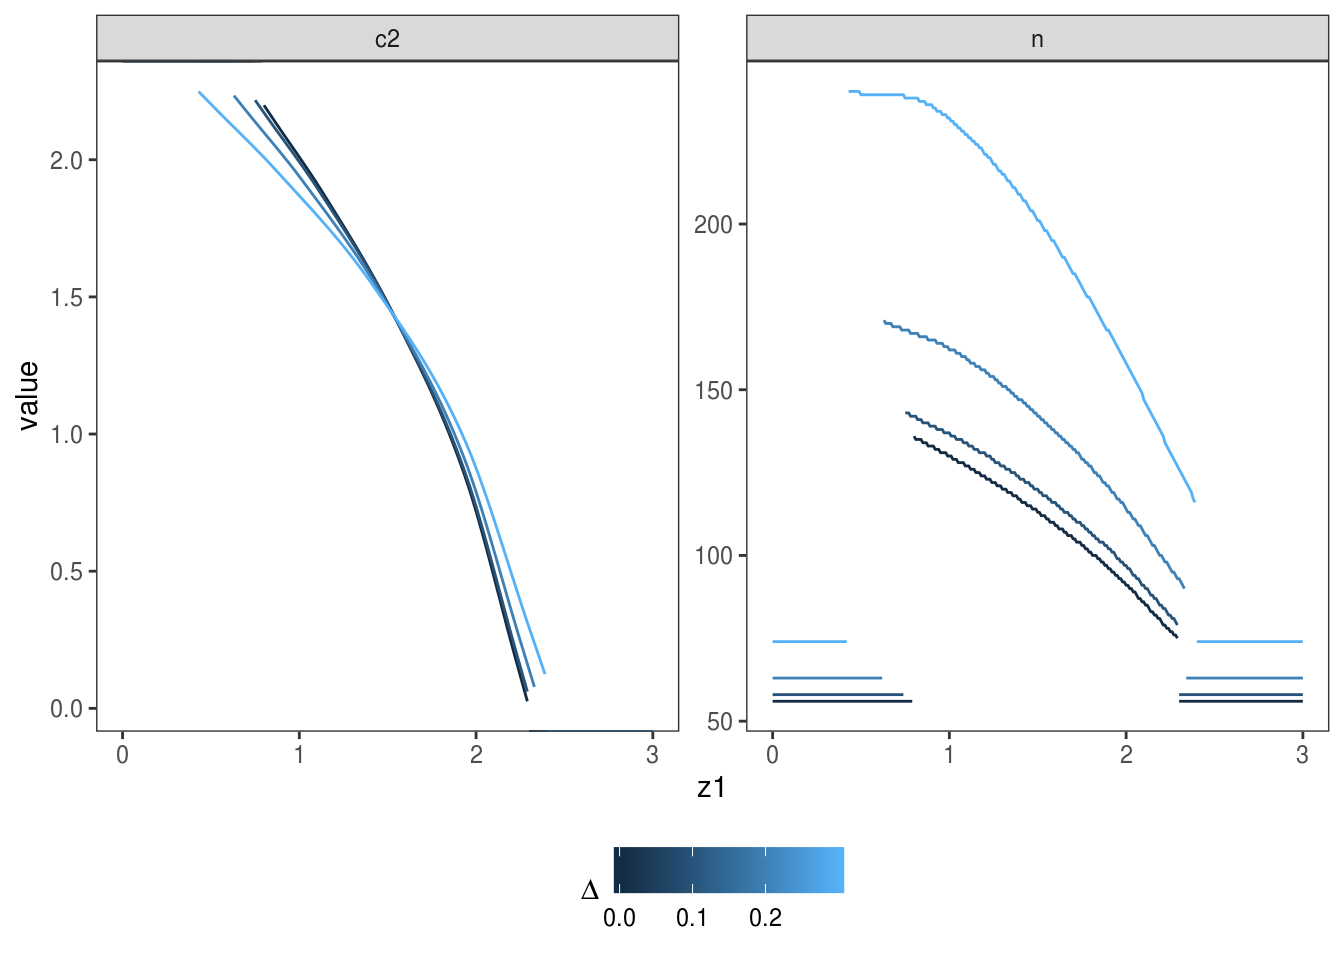
\includegraphics{adoptr-validation-report_files/figure-latex/unnamed-chunk-50-1.pdf}

\hypertarget{scenarioIV}{%
\chapter{Scenario IV: smaller effect, point prior}\label{scenarioIV}}

\hypertarget{details-3}{%
\section{Details}\label{details-3}}

In this scenario, we return to point priors as investigated in
\protect\hyperlink{scenarioI}{Scenario I}.
The main goal is to validate \texttt{adoptr}'s sensitivity with regards to
the assumed effect size and the constraints on power and type one error rate.

Therefore, we still assume a two-armed trial with normally distributed outcomes.
The assumed effect size becomes \(\delta = 0.2\) in this setting.
Type one error rate is protected at \(2.5\%\) and the power should be at least
\(80\%\). We will vary these values in the variants \protect\hyperlink{variantIV.2}{IV.2} and
\protect\hyperlink{variantIV.3}{IV.3}

\begin{Shaded}
\begin{Highlighting}[]
\CommentTok{# data distribution and hypotheses}
\NormalTok{datadist   <-}\StringTok{ }\KeywordTok{Normal}\NormalTok{(}\DataTypeTok{two_armed =} \OtherTok{TRUE}\NormalTok{)}
\NormalTok{H_}\DecValTok{0}\NormalTok{        <-}\StringTok{ }\KeywordTok{PointMassPrior}\NormalTok{(.}\DecValTok{0}\NormalTok{, }\DecValTok{1}\NormalTok{)}
\NormalTok{prior      <-}\StringTok{ }\KeywordTok{PointMassPrior}\NormalTok{(.}\DecValTok{2}\NormalTok{, }\DecValTok{1}\NormalTok{)}

\CommentTok{# constraints}
\NormalTok{alpha      <-}\StringTok{ }\FloatTok{0.025}
\NormalTok{min_power  <-}\StringTok{ }\FloatTok{0.8}
\NormalTok{toer_cnstr <-}\StringTok{ }\KeywordTok{Power}\NormalTok{(datadist, H_}\DecValTok{0}\NormalTok{)   }\OperatorTok{<=}\StringTok{ }\NormalTok{alpha}
\NormalTok{pow_cnstr  <-}\StringTok{ }\KeywordTok{Power}\NormalTok{(datadist, prior) }\OperatorTok{>=}\StringTok{ }\NormalTok{min_power}
\end{Highlighting}
\end{Shaded}

\hypertarget{variantIV_1}{%
\section{Variant IV-1: Minimizing Expected Sample Size under Point Prior}\label{variantIV_1}}

\hypertarget{objective-7}{%
\subsection{Objective}\label{objective-7}}

Expected sample size under the alternative point prior \(\delta = 0.2\)
is minimized.

\begin{Shaded}
\begin{Highlighting}[]
\NormalTok{ess <-}\StringTok{ }\KeywordTok{ExpectedSampleSize}\NormalTok{(datadist, prior)}
\end{Highlighting}
\end{Shaded}

\hypertarget{constraints-7}{%
\subsection{Constraints}\label{constraints-7}}

No additional constraints are considered in this variant.

\hypertarget{initial-design-5}{%
\subsection{Initial Design}\label{initial-design-5}}

For this example, the optimal one-stage, group-sequential, and generic
two-stage designs are computed.
The initial design that is used as starting value of optimization is defined
as a group-sequential design by the package \texttt{rpact} that fulfills
type one error rate and power constraints in the case of group-sequential and
two-stage design.
The initial one-stage design is chosen heuristically.
The order of integration is set to \(5\).

\begin{Shaded}
\begin{Highlighting}[]
\NormalTok{order <-}\StringTok{ }\NormalTok{5L }

\NormalTok{tbl_designs <-}\StringTok{ }\KeywordTok{tibble}\NormalTok{(}
    \DataTypeTok{type    =} \KeywordTok{c}\NormalTok{(}\StringTok{"one-stage"}\NormalTok{, }\StringTok{"group-sequential"}\NormalTok{, }\StringTok{"two-stage"}\NormalTok{),}
    \DataTypeTok{initial =} \KeywordTok{list}\NormalTok{(}
        \KeywordTok{OneStageDesign}\NormalTok{(}\DecValTok{500}\NormalTok{, }\FloatTok{2.0}\NormalTok{),}
        \KeywordTok{rpact_design}\NormalTok{(}\FloatTok{0.2}\NormalTok{, }\FloatTok{0.025}\NormalTok{, }\FloatTok{0.8}\NormalTok{, }\OtherTok{TRUE}\NormalTok{, order),}
        \KeywordTok{TwoStageDesign}\NormalTok{(}\KeywordTok{rpact_design}\NormalTok{(}\FloatTok{0.2}\NormalTok{, }\FloatTok{0.025}\NormalTok{, }\FloatTok{0.8}\NormalTok{, }\OtherTok{TRUE}\NormalTok{, order))) )}
\end{Highlighting}
\end{Shaded}

\hypertarget{optimization-6}{%
\subsection{Optimization}\label{optimization-6}}

\begin{Shaded}
\begin{Highlighting}[]
\NormalTok{tbl_designs <-}\StringTok{ }\NormalTok{tbl_designs }\OperatorTok\StringTok{ }
\StringTok{    }\KeywordTok{mutate}\NormalTok{(}
       \DataTypeTok{optimal =}\NormalTok{ purrr}\OperatorTok{::}\KeywordTok{map}\NormalTok{(initial, }\OperatorTok{~}\KeywordTok{minimize}\NormalTok{(}
         
\NormalTok{          ess,}
          \KeywordTok{subject_to}\NormalTok{(}
\NormalTok{              toer_cnstr,}
\NormalTok{              pow_cnstr}
\NormalTok{          ),}
          
          \DataTypeTok{initial_design =}\NormalTok{ ., }
          \DataTypeTok{opts           =}\NormalTok{ opts)) )}
\end{Highlighting}
\end{Shaded}

\hypertarget{test-cases-7}{%
\subsection{Test Cases}\label{test-cases-7}}

Firstly, it is checked whether the maximum number of iterations was
not exceeded in all three cases.

\begin{Shaded}
\begin{Highlighting}[]
\NormalTok{tbl_designs }\OperatorTok\StringTok{ }
\StringTok{  }\KeywordTok{transmute}\NormalTok{(}
\NormalTok{      type, }
      \DataTypeTok{iterations =}\NormalTok{ purrr}\OperatorTok{::}\KeywordTok{map_int}\NormalTok{(tbl_designs}\OperatorTok{$}\NormalTok{optimal, }
                                  \OperatorTok{~}\NormalTok{.}\OperatorTok{$}\NormalTok{nloptr_return}\OperatorTok{$}\NormalTok{iterations) ) }\OperatorTok
\StringTok{  }\NormalTok{\{}\KeywordTok{print}\NormalTok{(.); .\} }\OperatorTok\StringTok{ }
\StringTok{  }\NormalTok{\{testthat}\OperatorTok{::}\KeywordTok{expect_true}\NormalTok{(}\KeywordTok{all}\NormalTok{(.}\OperatorTok{$}\NormalTok{iterations }\OperatorTok{<}\StringTok{ }\NormalTok{opts}\OperatorTok{$}\NormalTok{maxeval))\}}
\end{Highlighting}
\end{Shaded}

\begin{verbatim}
## # A tibble: 3 x 2
##   type             iterations
##   <chr>                 <int>
## 1 one-stage                20
## 2 group-sequential        915
## 3 two-stage              2207
\end{verbatim}

Now, the constraints on type one error rate and power are tested via simulation.

\begin{Shaded}
\begin{Highlighting}[]
\NormalTok{tbl_designs }\OperatorTok\StringTok{ }
\StringTok{  }\KeywordTok{transmute}\NormalTok{(}
\NormalTok{      type, }
      \DataTypeTok{toer  =}\NormalTok{ purrr}\OperatorTok{::}\KeywordTok{map}\NormalTok{(tbl_designs}\OperatorTok{$}\NormalTok{optimal, }
                         \OperatorTok{~}\KeywordTok{sim_pr_reject}\NormalTok{(.[[}\DecValTok{1}\NormalTok{]], }\FloatTok{.0}\NormalTok{, datadist)}\OperatorTok{$}\NormalTok{prob), }
      \DataTypeTok{power =}\NormalTok{ purrr}\OperatorTok{::}\KeywordTok{map}\NormalTok{(tbl_designs}\OperatorTok{$}\NormalTok{optimal, }
                         \OperatorTok{~}\KeywordTok{sim_pr_reject}\NormalTok{(.[[}\DecValTok{1}\NormalTok{]], }\FloatTok{.2}\NormalTok{, datadist)}\OperatorTok{$}\NormalTok{prob) ) }\OperatorTok\StringTok{ }
\StringTok{  }\KeywordTok{unnest}\NormalTok{() }\OperatorTok\StringTok{ }
\StringTok{  }\NormalTok{\{}\KeywordTok{print}\NormalTok{(.); .\} }\OperatorTok\StringTok{ }\NormalTok{\{}
\NormalTok{  testthat}\OperatorTok{::}\KeywordTok{expect_true}\NormalTok{(}\KeywordTok{all}\NormalTok{(.}\OperatorTok{$}\NormalTok{toer  }\OperatorTok{<=}\StringTok{ }\NormalTok{alpha }\OperatorTok{*}\StringTok{ }\NormalTok{(}\DecValTok{1} \OperatorTok{+}\StringTok{ }\NormalTok{tol)))}
\NormalTok{  testthat}\OperatorTok{::}\KeywordTok{expect_true}\NormalTok{(}\KeywordTok{all}\NormalTok{(.}\OperatorTok{$}\NormalTok{power }\OperatorTok{>=}\StringTok{ }\NormalTok{min_power }\OperatorTok{*}\StringTok{ }\NormalTok{(}\DecValTok{1} \OperatorTok{-}\StringTok{ }\NormalTok{tol))) \}}
\end{Highlighting}
\end{Shaded}

\begin{verbatim}
## # A tibble: 3 x 3
##   type               toer power
##   <chr>             <dbl> <dbl>
## 1 one-stage        0.0251 0.799
## 2 group-sequential 0.0250 0.800
## 3 two-stage        0.0250 0.800
\end{verbatim}

Due to increasing degrees of freedom, the expected sample sizes under the
alternative should be ordered as `one-stage \textgreater{} group-sequential \textgreater{} two-stage'.
They are evaluated by simulation as well as by \texttt{evaluate()}.

\begin{Shaded}
\begin{Highlighting}[]
\NormalTok{tbl_designs }\OperatorTok\StringTok{ }
\StringTok{    }\KeywordTok{mutate}\NormalTok{(}
        \DataTypeTok{ess      =} \KeywordTok{map_dbl}\NormalTok{(optimal,}
                           \OperatorTok{~}\KeywordTok{evaluate}\NormalTok{(ess, .}\OperatorTok{$}\NormalTok{design) ),}
        \DataTypeTok{ess_sim  =} \KeywordTok{map_dbl}\NormalTok{(optimal,}
                           \OperatorTok{~}\KeywordTok{sim_n}\NormalTok{(.}\OperatorTok{$}\NormalTok{design, }\FloatTok{.2}\NormalTok{, datadist)}\OperatorTok{$}\NormalTok{n ) ) }\OperatorTok
\StringTok{    }\NormalTok{\{}\KeywordTok{print}\NormalTok{(.); .\} }\OperatorTok\StringTok{ }\NormalTok{\{}
    \CommentTok{# sim/evaluate same under alternative?}
\NormalTok{    testthat}\OperatorTok{::}\KeywordTok{expect_equal}\NormalTok{(.}\OperatorTok{$}\NormalTok{ess, .}\OperatorTok{$}\NormalTok{ess_sim, }
                           \DataTypeTok{tolerance =}\NormalTok{ tol_n,}
                           \DataTypeTok{scale =} \DecValTok{1}\NormalTok{)}
    \CommentTok{# monotonicity with respect to degrees of freedom}
\NormalTok{    testthat}\OperatorTok{::}\KeywordTok{expect_true}\NormalTok{(}\KeywordTok{all}\NormalTok{(}\KeywordTok{diff}\NormalTok{(.}\OperatorTok{$}\NormalTok{ess) }\OperatorTok{<}\StringTok{ }\DecValTok{0}\NormalTok{)) \}}
\end{Highlighting}
\end{Shaded}

\begin{verbatim}
## # A tibble: 3 x 5
##   type             initial    optimal      ess ess_sim
##   <chr>            <list>     <list>     <dbl>   <dbl>
## 1 one-stage        <OnStgDsg> <list [3]>  392     392 
## 2 group-sequential <GrpSqntD> <list [3]>  324.    323.
## 3 two-stage        <TwStgDsg> <list [3]>  319.    319.
\end{verbatim}

Furthermore, the expected sample size under the alternative of the
optimal group-sequential design should be lower than for the
group-sequential design by \texttt{rpact} that is based on the inverse normal
combination test.

\begin{Shaded}
\begin{Highlighting}[]
\NormalTok{tbl_designs }\OperatorTok
\StringTok{             }\KeywordTok{filter}\NormalTok{(type }\OperatorTok{==}\StringTok{ "group-sequential"}\NormalTok{) }\OperatorTok
\StringTok{             }\NormalTok{\{ }\KeywordTok{expect_lte}\NormalTok{(}
                 \KeywordTok{evaluate}\NormalTok{(ess, \{.[[}\StringTok{"optimal"}\NormalTok{]][[}\DecValTok{1}\NormalTok{]]}\OperatorTok{$}\NormalTok{design\}),}
                 \KeywordTok{evaluate}\NormalTok{(ess, \{.[[}\StringTok{"initial"}\NormalTok{]][[}\DecValTok{1}\NormalTok{]]\})}
\NormalTok{             ) \}}
\end{Highlighting}
\end{Shaded}

Finally, the \(n_2\) function of the optimal two-stage design is expected to be
monotonously decreasing:

\begin{Shaded}
\begin{Highlighting}[]
\KeywordTok{expect_true}\NormalTok{(}
    \KeywordTok{all}\NormalTok{(}\KeywordTok{diff}\NormalTok{(}
        \CommentTok{# get optimal two-stage design n2 pivots}
\NormalTok{        tbl_designs }\OperatorTok\StringTok{ }\KeywordTok{filter}\NormalTok{(type }\OperatorTok{==}\StringTok{ "two-stage"}\NormalTok{) }\OperatorTok
\StringTok{           }\NormalTok{\{.[[}\StringTok{"optimal"}\NormalTok{]][[}\DecValTok{1}\NormalTok{]]}\OperatorTok{$}\NormalTok{design}\OperatorTok{@}\NormalTok{n2_pivots\} }
\NormalTok{        ) }\OperatorTok{<}\StringTok{ }\DecValTok{0}\NormalTok{) )}
\end{Highlighting}
\end{Shaded}

\hypertarget{variantIV_2}{%
\section{Variant IV-2: Increase Power}\label{variantIV_2}}

\hypertarget{objective-8}{%
\subsection{Objective}\label{objective-8}}

The objective remains expected sample size under the alternative \(\delta = 0.2\).

\hypertarget{constraints-8}{%
\subsection{Constraints}\label{constraints-8}}

The minimal required power is increased to \(90\%\).

\begin{Shaded}
\begin{Highlighting}[]
\NormalTok{min_power_}\DecValTok{2}\NormalTok{ <-}\StringTok{ }\FloatTok{0.9}
\NormalTok{pow_cnstr_}\DecValTok{2}\NormalTok{ <-}\StringTok{ }\KeywordTok{Power}\NormalTok{(datadist, prior) }\OperatorTok{>=}\StringTok{ }\NormalTok{min_power_}\DecValTok{2}
\end{Highlighting}
\end{Shaded}

\hypertarget{initial-design-6}{%
\subsection{Initial Design}\label{initial-design-6}}

For both flavours with two stages (group-sequential, generic two-stage)
the initial design is created by \texttt{rpact} to fulfill the error rate constraints.

\begin{Shaded}
\begin{Highlighting}[]
\NormalTok{tbl_designs_}\DecValTok{9}\NormalTok{ <-}\StringTok{ }\KeywordTok{tibble}\NormalTok{(}
    \DataTypeTok{type    =} \KeywordTok{c}\NormalTok{(}\StringTok{"one-stage"}\NormalTok{, }\StringTok{"group-sequential"}\NormalTok{, }\StringTok{"two-stage"}\NormalTok{),}
    \DataTypeTok{initial =} \KeywordTok{list}\NormalTok{(}
        \KeywordTok{OneStageDesign}\NormalTok{(}\DecValTok{500}\NormalTok{, }\FloatTok{2.0}\NormalTok{),}
        \KeywordTok{rpact_design}\NormalTok{(}\FloatTok{0.2}\NormalTok{, }\FloatTok{0.025}\NormalTok{, }\FloatTok{0.9}\NormalTok{, }\OtherTok{TRUE}\NormalTok{, order),}
        \KeywordTok{TwoStageDesign}\NormalTok{(}\KeywordTok{rpact_design}\NormalTok{(}\FloatTok{0.2}\NormalTok{, }\FloatTok{0.025}\NormalTok{, }\FloatTok{0.9}\NormalTok{, }\OtherTok{TRUE}\NormalTok{, order))) )}
\end{Highlighting}
\end{Shaded}

\hypertarget{optimization-7}{%
\subsection{Optimization}\label{optimization-7}}

\begin{Shaded}
\begin{Highlighting}[]
\NormalTok{tbl_designs_}\DecValTok{9}\NormalTok{ <-}\StringTok{ }\NormalTok{tbl_designs_}\DecValTok{9} \OperatorTok\StringTok{ }
\StringTok{    }\KeywordTok{mutate}\NormalTok{(}
       \DataTypeTok{optimal =}\NormalTok{ purrr}\OperatorTok{::}\KeywordTok{map}\NormalTok{(initial, }\OperatorTok{~}\KeywordTok{minimize}\NormalTok{(}
         
\NormalTok{          ess,}
          \KeywordTok{subject_to}\NormalTok{(}
\NormalTok{              toer_cnstr,}
\NormalTok{              pow_cnstr_}\DecValTok{2}
\NormalTok{          ),}
          
          \DataTypeTok{initial_design =}\NormalTok{ ., }
          \DataTypeTok{opts           =}\NormalTok{ opts)) )}
\end{Highlighting}
\end{Shaded}

\hypertarget{test-cases-8}{%
\subsection{Test Cases}\label{test-cases-8}}

We start checking if the maximum number of iterations was not exceeded in all
three cases.

\begin{Shaded}
\begin{Highlighting}[]
\NormalTok{tbl_designs_}\DecValTok{9} \OperatorTok\StringTok{ }
\StringTok{  }\KeywordTok{transmute}\NormalTok{(}
\NormalTok{      type, }
      \DataTypeTok{iterations =}\NormalTok{ purrr}\OperatorTok{::}\KeywordTok{map_int}\NormalTok{(tbl_designs_}\DecValTok{9}\OperatorTok{$}\NormalTok{optimal, }
                                  \OperatorTok{~}\NormalTok{.}\OperatorTok{$}\NormalTok{nloptr_return}\OperatorTok{$}\NormalTok{iterations) ) }\OperatorTok
\StringTok{  }\NormalTok{\{}\KeywordTok{print}\NormalTok{(.); .\} }\OperatorTok\StringTok{ }
\StringTok{  }\NormalTok{\{testthat}\OperatorTok{::}\KeywordTok{expect_true}\NormalTok{(}\KeywordTok{all}\NormalTok{(.}\OperatorTok{$}\NormalTok{iterations }\OperatorTok{<}\StringTok{ }\NormalTok{opts}\OperatorTok{$}\NormalTok{maxeval))\}}
\end{Highlighting}
\end{Shaded}

\begin{verbatim}
## # A tibble: 3 x 2
##   type             iterations
##   <chr>                 <int>
## 1 one-stage                30
## 2 group-sequential       1349
## 3 two-stage              2988
\end{verbatim}

The type one error rate and pwoer constraints are evaluated by simulation.

\begin{Shaded}
\begin{Highlighting}[]
\NormalTok{tbl_designs_}\DecValTok{9} \OperatorTok\StringTok{ }
\StringTok{  }\KeywordTok{transmute}\NormalTok{(}
\NormalTok{      type, }
      \DataTypeTok{toer  =}\NormalTok{ purrr}\OperatorTok{::}\KeywordTok{map}\NormalTok{(tbl_designs_}\DecValTok{9}\OperatorTok{$}\NormalTok{optimal, }
                         \OperatorTok{~}\KeywordTok{sim_pr_reject}\NormalTok{(.[[}\DecValTok{1}\NormalTok{]], }\FloatTok{.0}\NormalTok{, datadist)}\OperatorTok{$}\NormalTok{prob), }
      \DataTypeTok{power =}\NormalTok{ purrr}\OperatorTok{::}\KeywordTok{map}\NormalTok{(tbl_designs_}\DecValTok{9}\OperatorTok{$}\NormalTok{optimal, }
                         \OperatorTok{~}\KeywordTok{sim_pr_reject}\NormalTok{(.[[}\DecValTok{1}\NormalTok{]], }\FloatTok{.2}\NormalTok{, datadist)}\OperatorTok{$}\NormalTok{prob) ) }\OperatorTok\StringTok{ }
\StringTok{  }\KeywordTok{unnest}\NormalTok{() }\OperatorTok\StringTok{ }
\StringTok{  }\NormalTok{\{}\KeywordTok{print}\NormalTok{(.); .\} }\OperatorTok\StringTok{ }\NormalTok{\{}
\NormalTok{  testthat}\OperatorTok{::}\KeywordTok{expect_true}\NormalTok{(}\KeywordTok{all}\NormalTok{(.}\OperatorTok{$}\NormalTok{toer  }\OperatorTok{<=}\StringTok{ }\NormalTok{alpha }\OperatorTok{*}\StringTok{ }\NormalTok{(}\DecValTok{1} \OperatorTok{+}\StringTok{ }\NormalTok{tol)))}
\NormalTok{  testthat}\OperatorTok{::}\KeywordTok{expect_true}\NormalTok{(}\KeywordTok{all}\NormalTok{(.}\OperatorTok{$}\NormalTok{power }\OperatorTok{>=}\StringTok{ }\NormalTok{min_power_}\DecValTok{2} \OperatorTok{*}\StringTok{ }\NormalTok{(}\DecValTok{1} \OperatorTok{-}\StringTok{ }\NormalTok{tol))) \}}
\end{Highlighting}
\end{Shaded}

\begin{verbatim}
## # A tibble: 3 x 3
##   type               toer power
##   <chr>             <dbl> <dbl>
## 1 one-stage        0.0251 0.900
## 2 group-sequential 0.0249 0.900
## 3 two-stage        0.0250 0.900
\end{verbatim}

Due to increasing degrees of freedom, the expected sample sizes under the
alternative should be ordered as `one-stage \textgreater{} group-sequential \textgreater{} two-stage'.
This is tested by simulation as well as by \texttt{evaluate()}.

\begin{Shaded}
\begin{Highlighting}[]
\NormalTok{tbl_designs_}\DecValTok{9} \OperatorTok\StringTok{ }
\StringTok{    }\KeywordTok{mutate}\NormalTok{(}
        \DataTypeTok{ess      =} \KeywordTok{map_dbl}\NormalTok{(optimal,}
                           \OperatorTok{~}\KeywordTok{evaluate}\NormalTok{(ess, .}\OperatorTok{$}\NormalTok{design) ),}
        \DataTypeTok{ess_sim  =} \KeywordTok{map_dbl}\NormalTok{(optimal,}
                           \OperatorTok{~}\KeywordTok{sim_n}\NormalTok{(.}\OperatorTok{$}\NormalTok{design, }\FloatTok{.2}\NormalTok{, datadist)}\OperatorTok{$}\NormalTok{n ) ) }\OperatorTok
\StringTok{    }\NormalTok{\{}\KeywordTok{print}\NormalTok{(.); .\} }\OperatorTok\StringTok{ }\NormalTok{\{}
    \CommentTok{# sim/evaluate same under alternative?}
\NormalTok{    testthat}\OperatorTok{::}\KeywordTok{expect_equal}\NormalTok{(.}\OperatorTok{$}\NormalTok{ess, .}\OperatorTok{$}\NormalTok{ess_sim, }
                           \DataTypeTok{tolerance =}\NormalTok{ tol_n,}
                           \DataTypeTok{scale =} \DecValTok{1}\NormalTok{)}
    \CommentTok{# monotonicity with respect to degrees of freedom}
\NormalTok{    testthat}\OperatorTok{::}\KeywordTok{expect_true}\NormalTok{(}\KeywordTok{all}\NormalTok{(}\KeywordTok{diff}\NormalTok{(.}\OperatorTok{$}\NormalTok{ess)     }\OperatorTok{<}\StringTok{ }\DecValTok{0}\NormalTok{)) }
\NormalTok{    testthat}\OperatorTok{::}\KeywordTok{expect_true}\NormalTok{(}\KeywordTok{all}\NormalTok{(}\KeywordTok{diff}\NormalTok{(.}\OperatorTok{$}\NormalTok{ess_sim) }\OperatorTok{<}\StringTok{ }\DecValTok{0}\NormalTok{))\}}
\end{Highlighting}
\end{Shaded}

\begin{verbatim}
## # A tibble: 3 x 5
##   type             initial    optimal      ess ess_sim
##   <chr>            <list>     <list>     <dbl>   <dbl>
## 1 one-stage        <OnStgDsg> <list [3]>  525     525 
## 2 group-sequential <GrpSqntD> <list [3]>  405.    405.
## 3 two-stage        <TwStgDsg> <list [3]>  397.    397.
\end{verbatim}

Comparing with the inverse-normal based group-sequential design created
by \texttt{rpact}, the optimal group-sequential design should show
a lower expected sample size under the point alternative.

\begin{Shaded}
\begin{Highlighting}[]
\NormalTok{tbl_designs_}\DecValTok{9} \OperatorTok
\StringTok{             }\KeywordTok{filter}\NormalTok{(type }\OperatorTok{==}\StringTok{ "group-sequential"}\NormalTok{) }\OperatorTok
\StringTok{             }\NormalTok{\{ }\KeywordTok{expect_lte}\NormalTok{(}
                 \KeywordTok{evaluate}\NormalTok{(ess, \{.[[}\StringTok{"optimal"}\NormalTok{]][[}\DecValTok{1}\NormalTok{]]}\OperatorTok{$}\NormalTok{design\}),}
                 \KeywordTok{evaluate}\NormalTok{(ess, \{.[[}\StringTok{"initial"}\NormalTok{]][[}\DecValTok{1}\NormalTok{]]\})}
\NormalTok{             ) \}}
\end{Highlighting}
\end{Shaded}

Since a point prior is regarded, the \(n_2\) function of the optimal
two-stage design is expected to be monotonously decreasing:

\begin{Shaded}
\begin{Highlighting}[]
\KeywordTok{expect_true}\NormalTok{(}
    \KeywordTok{all}\NormalTok{(}\KeywordTok{diff}\NormalTok{(}
        \CommentTok{# get optimal two-stage design n2 pivots}
\NormalTok{        tbl_designs_}\DecValTok{9} \OperatorTok\StringTok{ }\KeywordTok{filter}\NormalTok{(type }\OperatorTok{==}\StringTok{ "two-stage"}\NormalTok{) }\OperatorTok
\StringTok{           }\NormalTok{\{.[[}\StringTok{"optimal"}\NormalTok{]][[}\DecValTok{1}\NormalTok{]]}\OperatorTok{$}\NormalTok{design}\OperatorTok{@}\NormalTok{n2_pivots\} }
\NormalTok{        ) }\OperatorTok{<}\StringTok{ }\DecValTok{0}\NormalTok{) )}
\end{Highlighting}
\end{Shaded}

\hypertarget{variantIV_3}{%
\section{Variant IV-3: Increase Type One Error rate}\label{variantIV_3}}

\hypertarget{objective-9}{%
\subsection{Objective}\label{objective-9}}

As in variants \protect\hyperlink{variantIV_1}{IV.1} and \protect\hyperlink{variantIV_2}{IV-2},
expected sample size under the point alternative is minimized.

\hypertarget{constraints-9}{%
\subsection{Constraints}\label{constraints-9}}

While the power is still lower bounded by \(90\%\) as in variant \protect\hyperlink{variantIV_2}{II},
the maximal type one error rate is increased to \(5\%\).

\begin{Shaded}
\begin{Highlighting}[]
\NormalTok{alpha_}\DecValTok{2}\NormalTok{ <-}\StringTok{ }\FloatTok{.05}
\NormalTok{toer_cnstr_}\DecValTok{2}\NormalTok{ <-}\StringTok{ }\KeywordTok{Power}\NormalTok{(datadist, H_}\DecValTok{0}\NormalTok{) }\OperatorTok{<=}\StringTok{ }\NormalTok{alpha_}\DecValTok{2}
\end{Highlighting}
\end{Shaded}

\hypertarget{initial-design-7}{%
\subsection{Initial Design}\label{initial-design-7}}

Again, a design computed by means of the \texttt{rpact}-package to fulfill
the updated error rate constraints is applied as initial design for the
optimal group-sequential and generic two-stage designs.

\begin{Shaded}
\begin{Highlighting}[]
\NormalTok{tbl_designs_}\DecValTok{5}\NormalTok{ <-}\StringTok{ }\KeywordTok{tibble}\NormalTok{(}
    \DataTypeTok{type    =} \KeywordTok{c}\NormalTok{(}\StringTok{"one-stage"}\NormalTok{, }\StringTok{"group-sequential"}\NormalTok{, }\StringTok{"two-stage"}\NormalTok{),}
    \DataTypeTok{initial =} \KeywordTok{list}\NormalTok{(}
        \KeywordTok{OneStageDesign}\NormalTok{(}\DecValTok{500}\NormalTok{, }\FloatTok{2.0}\NormalTok{),}
        \KeywordTok{rpact_design}\NormalTok{(}\FloatTok{0.2}\NormalTok{, }\FloatTok{0.05}\NormalTok{, }\FloatTok{0.9}\NormalTok{, }\OtherTok{TRUE}\NormalTok{, order),}
        \KeywordTok{TwoStageDesign}\NormalTok{(}\KeywordTok{rpact_design}\NormalTok{(}\FloatTok{0.2}\NormalTok{, }\FloatTok{0.05}\NormalTok{, }\FloatTok{0.9}\NormalTok{, }\OtherTok{TRUE}\NormalTok{, order))) )}
\end{Highlighting}
\end{Shaded}

\hypertarget{optimization-8}{%
\subsection{Optimization}\label{optimization-8}}

\begin{Shaded}
\begin{Highlighting}[]
\NormalTok{tbl_designs_}\DecValTok{5}\NormalTok{ <-}\StringTok{ }\NormalTok{tbl_designs_}\DecValTok{5} \OperatorTok\StringTok{ }
\StringTok{    }\KeywordTok{mutate}\NormalTok{(}
       \DataTypeTok{optimal =}\NormalTok{ purrr}\OperatorTok{::}\KeywordTok{map}\NormalTok{(initial, }\OperatorTok{~}\KeywordTok{minimize}\NormalTok{(}
         
\NormalTok{          ess,}
          \KeywordTok{subject_to}\NormalTok{(}
\NormalTok{              toer_cnstr_}\DecValTok{2}\NormalTok{,}
\NormalTok{              pow_cnstr_}\DecValTok{2}
\NormalTok{          ),}
          
          \DataTypeTok{initial_design =}\NormalTok{ ., }
          \DataTypeTok{opts           =}\NormalTok{ opts)) )}
\end{Highlighting}
\end{Shaded}

\hypertarget{test-cases-9}{%
\subsection{Test Cases}\label{test-cases-9}}

The convergence of the optimization algorithm is tested by checking if the
maximum number of iterations was not exceeded.

\begin{Shaded}
\begin{Highlighting}[]
\NormalTok{tbl_designs_}\DecValTok{5} \OperatorTok\StringTok{ }
\StringTok{  }\KeywordTok{transmute}\NormalTok{(}
\NormalTok{      type, }
      \DataTypeTok{iterations =}\NormalTok{ purrr}\OperatorTok{::}\KeywordTok{map_int}\NormalTok{(tbl_designs_}\DecValTok{5}\OperatorTok{$}\NormalTok{optimal, }
                                  \OperatorTok{~}\NormalTok{.}\OperatorTok{$}\NormalTok{nloptr_return}\OperatorTok{$}\NormalTok{iterations) ) }\OperatorTok
\StringTok{  }\NormalTok{\{}\KeywordTok{print}\NormalTok{(.); .\} }\OperatorTok\StringTok{ }
\StringTok{  }\NormalTok{\{testthat}\OperatorTok{::}\KeywordTok{expect_true}\NormalTok{(}\KeywordTok{all}\NormalTok{(.}\OperatorTok{$}\NormalTok{iterations }\OperatorTok{<}\StringTok{ }\NormalTok{opts}\OperatorTok{$}\NormalTok{maxeval))\}}
\end{Highlighting}
\end{Shaded}

\begin{verbatim}
## # A tibble: 3 x 2
##   type             iterations
##   <chr>                 <int>
## 1 one-stage                27
## 2 group-sequential       1124
## 3 two-stage              2833
\end{verbatim}

By simulation, the constraints on the error rates (type one error and power)
are tested.

\begin{Shaded}
\begin{Highlighting}[]
\NormalTok{tbl_designs_}\DecValTok{5} \OperatorTok\StringTok{ }
\StringTok{  }\KeywordTok{transmute}\NormalTok{(}
\NormalTok{      type, }
      \DataTypeTok{toer  =}\NormalTok{ purrr}\OperatorTok{::}\KeywordTok{map}\NormalTok{(tbl_designs_}\DecValTok{5}\OperatorTok{$}\NormalTok{optimal, }
                         \OperatorTok{~}\KeywordTok{sim_pr_reject}\NormalTok{(.[[}\DecValTok{1}\NormalTok{]], }\FloatTok{.0}\NormalTok{, datadist)}\OperatorTok{$}\NormalTok{prob), }
      \DataTypeTok{power =}\NormalTok{ purrr}\OperatorTok{::}\KeywordTok{map}\NormalTok{(tbl_designs_}\DecValTok{5}\OperatorTok{$}\NormalTok{optimal, }
                         \OperatorTok{~}\KeywordTok{sim_pr_reject}\NormalTok{(.[[}\DecValTok{1}\NormalTok{]], }\FloatTok{.2}\NormalTok{, datadist)}\OperatorTok{$}\NormalTok{prob) ) }\OperatorTok\StringTok{ }
\StringTok{  }\KeywordTok{unnest}\NormalTok{() }\OperatorTok\StringTok{ }
\StringTok{  }\NormalTok{\{}\KeywordTok{print}\NormalTok{(.); .\} }\OperatorTok\StringTok{ }\NormalTok{\{}
\NormalTok{  testthat}\OperatorTok{::}\KeywordTok{expect_true}\NormalTok{(}\KeywordTok{all}\NormalTok{(.}\OperatorTok{$}\NormalTok{toer  }\OperatorTok{<=}\StringTok{ }\NormalTok{alpha_}\DecValTok{2} \OperatorTok{*}\StringTok{ }\NormalTok{(}\DecValTok{1} \OperatorTok{+}\StringTok{ }\NormalTok{tol)))}
\NormalTok{  testthat}\OperatorTok{::}\KeywordTok{expect_true}\NormalTok{(}\KeywordTok{all}\NormalTok{(.}\OperatorTok{$}\NormalTok{power }\OperatorTok{>=}\StringTok{ }\NormalTok{min_power_}\DecValTok{2} \OperatorTok{*}\StringTok{ }\NormalTok{(}\DecValTok{1} \OperatorTok{-}\StringTok{ }\NormalTok{tol))) \}}
\end{Highlighting}
\end{Shaded}

\begin{verbatim}
## # A tibble: 3 x 3
##   type               toer power
##   <chr>             <dbl> <dbl>
## 1 one-stage        0.0502 0.900
## 2 group-sequential 0.0500 0.900
## 3 two-stage        0.0502 0.900
\end{verbatim}

Due to increasing degrees of freedom, the expected sample sizes under the
alternative should be ordered as `one-stage \textgreater{} group-sequential \textgreater{} two-stage'.
They are tested by simulation as well as by calling \texttt{evaluate()}.

\begin{Shaded}
\begin{Highlighting}[]
\NormalTok{tbl_designs_}\DecValTok{5} \OperatorTok\StringTok{ }
\StringTok{    }\KeywordTok{mutate}\NormalTok{(}
        \DataTypeTok{ess      =} \KeywordTok{map_dbl}\NormalTok{(optimal,}
                           \OperatorTok{~}\KeywordTok{evaluate}\NormalTok{(ess, .}\OperatorTok{$}\NormalTok{design) ),}
        \DataTypeTok{ess_sim  =} \KeywordTok{map_dbl}\NormalTok{(optimal,}
                           \OperatorTok{~}\KeywordTok{sim_n}\NormalTok{(.}\OperatorTok{$}\NormalTok{design, }\FloatTok{.2}\NormalTok{, datadist)}\OperatorTok{$}\NormalTok{n ) ) }\OperatorTok
\StringTok{    }\NormalTok{\{}\KeywordTok{print}\NormalTok{(.); .\} }\OperatorTok\StringTok{ }\NormalTok{\{}
    \CommentTok{# sim/evaluate same under alternative?}
\NormalTok{    testthat}\OperatorTok{::}\KeywordTok{expect_equal}\NormalTok{(.}\OperatorTok{$}\NormalTok{ess, .}\OperatorTok{$}\NormalTok{ess_sim, }
                           \DataTypeTok{tolerance =}\NormalTok{ tol_n,}
                           \DataTypeTok{scale =} \DecValTok{1}\NormalTok{)}
    \CommentTok{# monotonicity with respect to degrees of freedom}
\NormalTok{    testthat}\OperatorTok{::}\KeywordTok{expect_true}\NormalTok{(}\KeywordTok{all}\NormalTok{(}\KeywordTok{diff}\NormalTok{(.}\OperatorTok{$}\NormalTok{ess) }\OperatorTok{<}\StringTok{ }\DecValTok{0}\NormalTok{)) \}}
\end{Highlighting}
\end{Shaded}

\begin{verbatim}
## # A tibble: 3 x 5
##   type             initial    optimal      ess ess_sim
##   <chr>            <list>     <list>     <dbl>   <dbl>
## 1 one-stage        <OnStgDsg> <list [3]>  428     428 
## 2 group-sequential <GrpSqntD> <list [3]>  326.    325.
## 3 two-stage        <TwStgDsg> <list [3]>  319.    319.
\end{verbatim}

The expected sample size under the alternative that was used as objective criterion
of the optimal group-sequential design should be lower than for the
group-sequential design by \texttt{rpact} that is based on the inverse normal
combination test.

\begin{Shaded}
\begin{Highlighting}[]
\NormalTok{tbl_designs_}\DecValTok{5} \OperatorTok
\StringTok{             }\KeywordTok{filter}\NormalTok{(type }\OperatorTok{==}\StringTok{ "group-sequential"}\NormalTok{) }\OperatorTok
\StringTok{             }\NormalTok{\{ }\KeywordTok{expect_lte}\NormalTok{(}
                 \KeywordTok{evaluate}\NormalTok{(ess, \{.[[}\StringTok{"optimal"}\NormalTok{]][[}\DecValTok{1}\NormalTok{]]}\OperatorTok{$}\NormalTok{design\}),}
                 \KeywordTok{evaluate}\NormalTok{(ess, \{.[[}\StringTok{"initial"}\NormalTok{]][[}\DecValTok{1}\NormalTok{]]\})}
\NormalTok{             ) \}}
\end{Highlighting}
\end{Shaded}

Also in this variant, the \(n_2\) function of the optimal two-stage design
is expected to be monotonously decreasing:

\begin{Shaded}
\begin{Highlighting}[]
\KeywordTok{expect_true}\NormalTok{(}
    \KeywordTok{all}\NormalTok{(}\KeywordTok{diff}\NormalTok{(}
        \CommentTok{# get optimal two-stage design n2 pivots}
\NormalTok{        tbl_designs_}\DecValTok{5} \OperatorTok\StringTok{ }\KeywordTok{filter}\NormalTok{(type }\OperatorTok{==}\StringTok{ "two-stage"}\NormalTok{) }\OperatorTok
\StringTok{           }\NormalTok{\{.[[}\StringTok{"optimal"}\NormalTok{]][[}\DecValTok{1}\NormalTok{]]}\OperatorTok{$}\NormalTok{design}\OperatorTok{@}\NormalTok{n2_pivots\} }
\NormalTok{        ) }\OperatorTok{<}\StringTok{ }\DecValTok{0}\NormalTok{) )}
\end{Highlighting}
\end{Shaded}

\hypertarget{plot-two-stage-designs-2}{%
\section{Plot Two-Stage Designs}\label{plot-two-stage-designs-2}}

The optimal two-stage designs stemming from the three different variants
are plotted together.

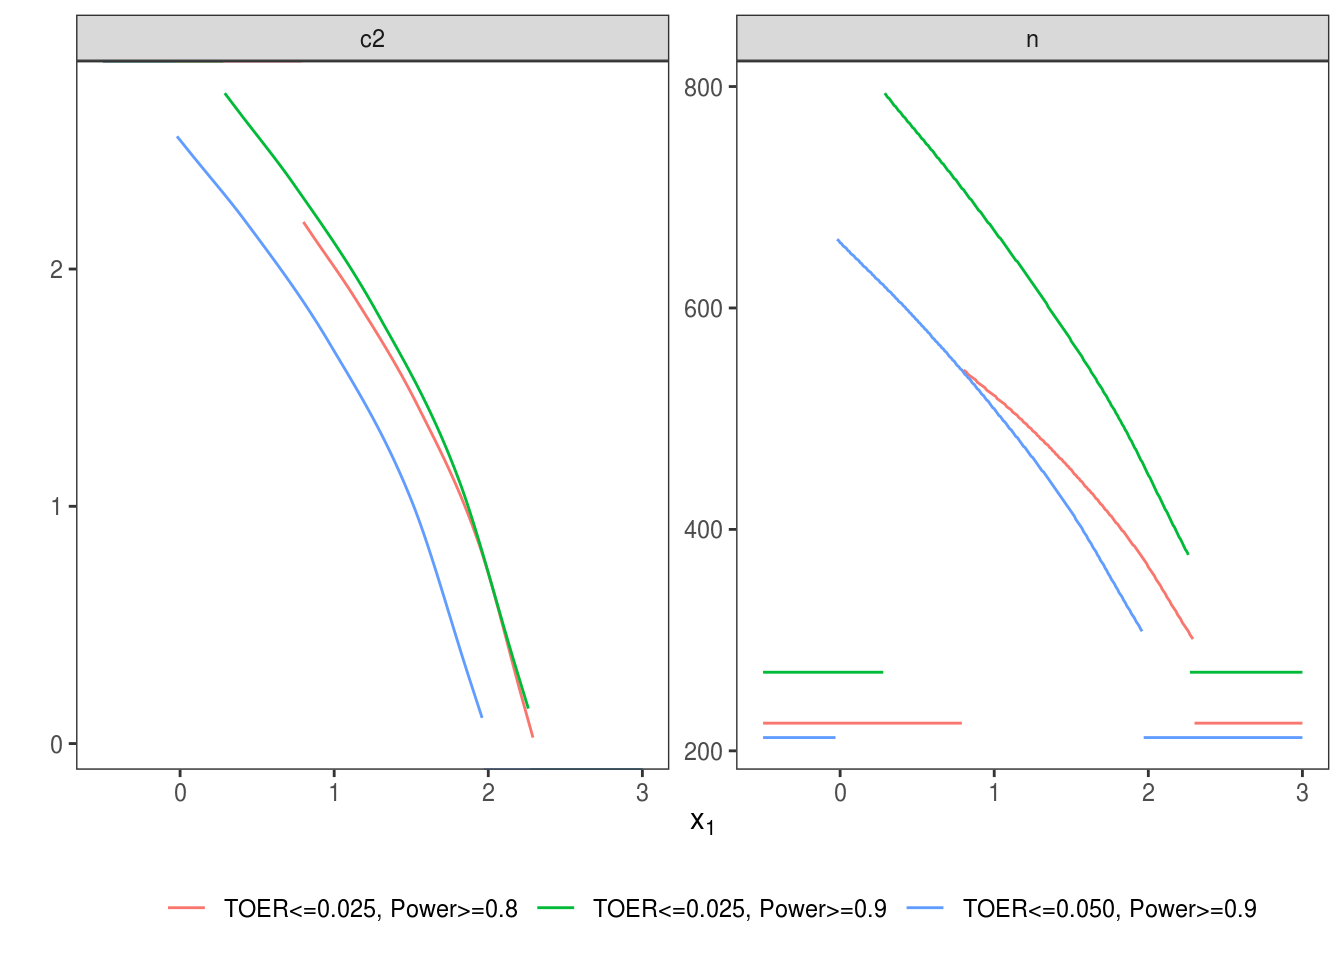
\includegraphics{adoptr-validation-report_files/figure-latex/unnamed-chunk-75-1.pdf}

\hypertarget{scenarioV}{%
\chapter{Scenario V: Single-arm design, medium effect size}\label{scenarioV}}

\hypertarget{details-4}{%
\section{Details}\label{details-4}}

In this scenario, a classical two-arm trial with normal
test statistic and known variance (w.l.o.g. variance of
the test statistic is 1).
This situation corresponds to a classical \(z\)-test for
a difference in population means.

\begin{Shaded}
\begin{Highlighting}[]
\NormalTok{datadist <-}\StringTok{ }\KeywordTok{Normal}\NormalTok{(}\DataTypeTok{two_armed =} \OtherTok{TRUE}\NormalTok{)}
\end{Highlighting}
\end{Shaded}

The null hypothesis is no population mean difference, i.e.
\(\mathcal{H}_0:\delta \leq 0\).

\begin{Shaded}
\begin{Highlighting}[]
\NormalTok{H_}\DecValTok{0}\NormalTok{ <-}\StringTok{ }\KeywordTok{PointMassPrior}\NormalTok{(.}\DecValTok{0}\NormalTok{, }\DecValTok{1}\NormalTok{)}
\end{Highlighting}
\end{Shaded}

An alternative effect size of \(\delta = 0.3\) with
point prior distribution is assumed.

\begin{Shaded}
\begin{Highlighting}[]
\NormalTok{prior <-}\StringTok{ }\KeywordTok{PointMassPrior}\NormalTok{(.}\DecValTok{3}\NormalTok{, }\DecValTok{1}\NormalTok{)}
\end{Highlighting}
\end{Shaded}

Across all variants in this scenario, the one-sided maximal
type one error rate is restricted to

\begin{Shaded}
\begin{Highlighting}[]
\NormalTok{alpha <-}\StringTok{ }\FloatTok{0.025}
\end{Highlighting}
\end{Shaded}

and the power at the point alternative of \(\delta=0.3\) must
be at least

\begin{Shaded}
\begin{Highlighting}[]
\NormalTok{min_power <-}\StringTok{ }\FloatTok{0.8}
\end{Highlighting}
\end{Shaded}

I.e. throughout this sceanrio, we always use the two
constraints

\begin{Shaded}
\begin{Highlighting}[]
\NormalTok{toer_cnstr <-}\StringTok{ }\KeywordTok{Power}\NormalTok{(datadist, H_}\DecValTok{0}\NormalTok{) }\OperatorTok{<=}\StringTok{ }\NormalTok{alpha}
\end{Highlighting}
\end{Shaded}

and

\begin{Shaded}
\begin{Highlighting}[]
\NormalTok{pow_cnstr <-}\StringTok{ }\KeywordTok{Power}\NormalTok{(datadist, prior) }\OperatorTok{>=}\StringTok{ }\NormalTok{min_power}
\end{Highlighting}
\end{Shaded}

\hypertarget{variantV_1}{%
\section{Variant V-1, sensitivity to integration order}\label{variantV_1}}

\hypertarget{objective-10}{%
\subsection{Objective}\label{objective-10}}

Expected sample size under the respective prior is minimized, i.e.,
\(\boldsymbol{E}\big[n(\mathcal{D})\big]\).

\begin{Shaded}
\begin{Highlighting}[]
\NormalTok{ess <-}\StringTok{ }\KeywordTok{ExpectedSampleSize}\NormalTok{(datadist, prior)}
\end{Highlighting}
\end{Shaded}

\hypertarget{constraints-10}{%
\subsection{Constraints}\label{constraints-10}}

No additional constraints are considered in this variant.

\hypertarget{initial-design-8}{%
\subsection{Initial Design}\label{initial-design-8}}

A fixed design for these parameters would require
176
subjects per group. We use the half of this as initial values for the
sample sizes.
The initial stop for futility is at \(c_1^f=0\), i.e., if the effect shows
in the opponent direction to the alternative.
The starting values for the efficacy stop and for \(c_2\) is the \(1-\alpha\)-
quantile of the normal distribution.

\begin{Shaded}
\begin{Highlighting}[]
\NormalTok{init_design <-}\StringTok{ }\ControlFlowTok{function}\NormalTok{(order) \{}
    \KeywordTok{TwoStageDesign}\NormalTok{(}
        \DataTypeTok{n1 =} \KeywordTok{ceiling}\NormalTok{(pwr}\OperatorTok{::}\KeywordTok{pwr.t.test}\NormalTok{(}\DataTypeTok{d =} \FloatTok{.3}\NormalTok{, }
                                     \DataTypeTok{sig.level =} \FloatTok{.025}\NormalTok{, }
                                     \DataTypeTok{power =} \FloatTok{.8}\NormalTok{, }
                                     \DataTypeTok{alternative =} \StringTok{"greater"}\NormalTok{)}\OperatorTok{$}\NormalTok{n) }\OperatorTok{/}\StringTok{ }\DecValTok{2}\NormalTok{,}
        \DataTypeTok{c1f =} \DecValTok{0}\NormalTok{,}
        \DataTypeTok{c1e =} \KeywordTok{qnorm}\NormalTok{( }\DecValTok{1} \OperatorTok{-}\StringTok{ }\FloatTok{0.025}\NormalTok{),}
        \DataTypeTok{n2 =} \KeywordTok{ceiling}\NormalTok{(pwr}\OperatorTok{::}\KeywordTok{pwr.t.test}\NormalTok{(}\DataTypeTok{d =} \FloatTok{.3}\NormalTok{, }
                                     \DataTypeTok{sig.level =} \FloatTok{.025}\NormalTok{, }
                                     \DataTypeTok{power =} \FloatTok{.8}\NormalTok{, }
                                     \DataTypeTok{alternative =} \StringTok{"greater"}\NormalTok{)}\OperatorTok{$}\NormalTok{n) }\OperatorTok{/}\StringTok{ }\DecValTok{2}\NormalTok{,}
        \DataTypeTok{c2 =} \KeywordTok{qnorm}\NormalTok{(}\DecValTok{1} \OperatorTok{-}\StringTok{ }\FloatTok{0.025}\NormalTok{),}
        \DataTypeTok{order =}\NormalTok{ order}
\NormalTok{)}
\NormalTok{\}}
\end{Highlighting}
\end{Shaded}

\hypertarget{optimization-9}{%
\subsection{Optimization}\label{optimization-9}}

The optimal design is computed for three different integration orders: 5, 8,
and 11.

\begin{Shaded}
\begin{Highlighting}[]
\NormalTok{opt_design <-}\StringTok{ }\ControlFlowTok{function}\NormalTok{(order) \{}
    \KeywordTok{minimize}\NormalTok{(}
\NormalTok{        ess,}
        \KeywordTok{subject_to}\NormalTok{(}
\NormalTok{            toer_cnstr,}
\NormalTok{            pow_cnstr}
\NormalTok{        ),}
        \DataTypeTok{initial_design =} \KeywordTok{init_design}\NormalTok{(order),}
        \DataTypeTok{opts =}\NormalTok{ opts}
\NormalTok{    )}
\NormalTok{\}}

\NormalTok{opt1 <-}\StringTok{ }\KeywordTok{lapply}\NormalTok{(}\KeywordTok{c}\NormalTok{(}\DecValTok{5}\NormalTok{, }\DecValTok{8}\NormalTok{, }\DecValTok{11}\NormalTok{), }\ControlFlowTok{function}\NormalTok{(x) }\KeywordTok{opt_design}\NormalTok{(x))}
\end{Highlighting}
\end{Shaded}

\hypertarget{test-cases-10}{%
\subsection{Test cases}\label{test-cases-10}}

Check if the optimization algorithm converged in all cases.

\begin{Shaded}
\begin{Highlighting}[]
\NormalTok{iters <-}\StringTok{ }\KeywordTok{sapply}\NormalTok{(opt1, }\ControlFlowTok{function}\NormalTok{(x) x}\OperatorTok{$}\NormalTok{nloptr_return}\OperatorTok{$}\NormalTok{iterations)}

\KeywordTok{print}\NormalTok{(iters)}
\end{Highlighting}
\end{Shaded}

\begin{verbatim}
## [1] 2328 4226 8913
\end{verbatim}

\begin{Shaded}
\begin{Highlighting}[]
\NormalTok{testthat}\OperatorTok{::}\KeywordTok{expect_true}\NormalTok{(}\KeywordTok{all}\NormalTok{(iters }\OperatorTok{<}\StringTok{ }\NormalTok{opts}\OperatorTok{$}\NormalTok{maxeval))}
\end{Highlighting}
\end{Shaded}

Check type one error rate control.

\begin{Shaded}
\begin{Highlighting}[]
\NormalTok{tmp     <-}\StringTok{ }\KeywordTok{sapply}\NormalTok{(opt1, }\ControlFlowTok{function}\NormalTok{(x) }\KeywordTok{sim_pr_reject}\NormalTok{(x}\OperatorTok{$}\NormalTok{design, }\FloatTok{.0}\NormalTok{, datadist))}
\NormalTok{df_toer <-}\StringTok{ }\KeywordTok{data.frame}\NormalTok{(}
    \DataTypeTok{toer =} \KeywordTok{as.numeric}\NormalTok{(tmp[}\DecValTok{1}\NormalTok{, ]),}
    \DataTypeTok{se   =} \KeywordTok{as.numeric}\NormalTok{(tmp[}\DecValTok{2}\NormalTok{, ])}
\NormalTok{)}
\KeywordTok{rm}\NormalTok{(tmp)}

\NormalTok{testthat}\OperatorTok{::}\KeywordTok{expect_true}\NormalTok{(}\KeywordTok{all}\NormalTok{(df_toer}\OperatorTok{$}\NormalTok{toer }\OperatorTok{<=}\StringTok{ }\NormalTok{alpha }\OperatorTok{*}\StringTok{ }\NormalTok{(}\DecValTok{1} \OperatorTok{+}\StringTok{ }\NormalTok{tol)))}

\NormalTok{df_toer}
\end{Highlighting}
\end{Shaded}

\begin{verbatim}
##       toer           se
## 1 0.024975 0.0001560489
## 2 0.024956 0.0001559911
## 3 0.024950 0.0001559728
\end{verbatim}

Check the power constraint.

\begin{Shaded}
\begin{Highlighting}[]
\NormalTok{tmp     <-}\StringTok{ }\KeywordTok{sapply}\NormalTok{(opt1, }\ControlFlowTok{function}\NormalTok{(x) }\KeywordTok{sim_pr_reject}\NormalTok{(x}\OperatorTok{$}\NormalTok{design, }\FloatTok{.3}\NormalTok{, datadist))}
\NormalTok{df_pow  <-}\StringTok{ }\KeywordTok{data.frame}\NormalTok{(}
    \DataTypeTok{power =} \KeywordTok{as.numeric}\NormalTok{(tmp[}\DecValTok{1}\NormalTok{, ]),}
    \DataTypeTok{se    =} \KeywordTok{as.numeric}\NormalTok{(tmp[}\DecValTok{2}\NormalTok{, ])}
\NormalTok{)}
\KeywordTok{rm}\NormalTok{(tmp)}

\NormalTok{testthat}\OperatorTok{::}\KeywordTok{expect_true}\NormalTok{(}\KeywordTok{all}\NormalTok{(df_pow}\OperatorTok{$}\NormalTok{pow }\OperatorTok{>=}\StringTok{ }\NormalTok{min_power }\OperatorTok{*}\StringTok{ }\NormalTok{(}\DecValTok{1} \OperatorTok{-}\StringTok{ }\NormalTok{tol)))}

\NormalTok{df_pow}
\end{Highlighting}
\end{Shaded}

\begin{verbatim}
##      power           se
## 1 0.799791 0.0004001569
## 2 0.799696 0.0004002280
## 3 0.799678 0.0004002415
\end{verbatim}

Check expected sample size under the prior.

\begin{Shaded}
\begin{Highlighting}[]
\NormalTok{tmp    <-}\StringTok{ }\KeywordTok{sapply}\NormalTok{(opt1, }\ControlFlowTok{function}\NormalTok{(x) }\KeywordTok{sim_n}\NormalTok{(x}\OperatorTok{$}\NormalTok{design, }\FloatTok{.3}\NormalTok{, datadist))}
\NormalTok{df_ess <-}\StringTok{ }\KeywordTok{data.frame}\NormalTok{(}
    \DataTypeTok{n  =} \KeywordTok{as.numeric}\NormalTok{(tmp[}\DecValTok{1}\NormalTok{, ]),}
    \DataTypeTok{se =} \KeywordTok{as.numeric}\NormalTok{(tmp[}\DecValTok{2}\NormalTok{, ])}
\NormalTok{)}
\KeywordTok{rm}\NormalTok{(tmp)}

\NormalTok{df_ess}
\end{Highlighting}
\end{Shaded}

\begin{verbatim}
##          n         se
## 1 141.9614 0.04874384
## 2 141.9801 0.04875722
## 3 141.9822 0.04875670
\end{verbatim}

\hypertarget{variantV_2}{%
\section{Variant V-2, utility maximization}\label{variantV_2}}

\hypertarget{objective-11}{%
\subsection{Objective}\label{objective-11}}

In this case, a utility function consisting of expected sample size and
power is minimized.

\begin{Shaded}
\begin{Highlighting}[]
\NormalTok{pow <-}\StringTok{ }\KeywordTok{Power}\NormalTok{(datadist, prior)}
\NormalTok{ess <-}\StringTok{ }\KeywordTok{ExpectedSampleSize}\NormalTok{(datadist, prior)}

\NormalTok{obj <-}\StringTok{ }\ControlFlowTok{function}\NormalTok{(lambda) \{}
  \KeywordTok{composite}\NormalTok{(\{ess }\OperatorTok{-}\StringTok{ }\NormalTok{lambda }\OperatorTok{*}\StringTok{ }\NormalTok{pow\})}
\NormalTok{\}}
\end{Highlighting}
\end{Shaded}

\hypertarget{constraints-11}{%
\subsection{Constraints}\label{constraints-11}}

The type one error rate is controlled at 0.025 on the boundary of the
null hypothesis. Hence, the previous inequality can still be used.
There is no constraint on power anymore because power is part of the
objective utility function.

\hypertarget{initial-design-9}{%
\subsection{Initial Design}\label{initial-design-9}}

The previous initial design with order \(5\) is applied.

\hypertarget{optimization-10}{%
\subsection{Optimization}\label{optimization-10}}

The optimal design is computed for two values of \(\lambda\): 200 and 500.

\begin{Shaded}
\begin{Highlighting}[]
\NormalTok{opt2_design <-}\StringTok{ }\ControlFlowTok{function}\NormalTok{(lambda) \{}

    \KeywordTok{minimize}\NormalTok{(}
        \KeywordTok{obj}\NormalTok{(lambda),}
        \KeywordTok{subject_to}\NormalTok{(}
\NormalTok{            toer_cnstr}
\NormalTok{        ),}
        \DataTypeTok{initial_design =} \KeywordTok{init_design}\NormalTok{(}\DecValTok{5}\NormalTok{),}
        \DataTypeTok{opts =}\NormalTok{ opts}
\NormalTok{    )}
\NormalTok{\}}

\NormalTok{opt2 <-}\StringTok{ }\KeywordTok{lapply}\NormalTok{(}\KeywordTok{c}\NormalTok{(}\DecValTok{200}\NormalTok{, }\DecValTok{500}\NormalTok{), }\ControlFlowTok{function}\NormalTok{(x) }\KeywordTok{opt2_design}\NormalTok{(x))}
\end{Highlighting}
\end{Shaded}

\hypertarget{test-cases-11}{%
\subsection{Test cases}\label{test-cases-11}}

Check if the optimization algorithm converged in all cases.

\begin{Shaded}
\begin{Highlighting}[]
\NormalTok{iters <-}\StringTok{ }\KeywordTok{sapply}\NormalTok{(opt2, }\ControlFlowTok{function}\NormalTok{(x) x}\OperatorTok{$}\NormalTok{nloptr_return}\OperatorTok{$}\NormalTok{iterations)}

\KeywordTok{print}\NormalTok{(iters)}
\end{Highlighting}
\end{Shaded}

\begin{verbatim}
## [1]  2062 13606
\end{verbatim}

\begin{Shaded}
\begin{Highlighting}[]
\NormalTok{testthat}\OperatorTok{::}\KeywordTok{expect_true}\NormalTok{(}\KeywordTok{all}\NormalTok{(iters }\OperatorTok{<}\StringTok{ }\NormalTok{opts}\OperatorTok{$}\NormalTok{maxeval))}
\end{Highlighting}
\end{Shaded}

Check type one error rate control for both designs via simulation.

\begin{Shaded}
\begin{Highlighting}[]
\NormalTok{tmp     <-}\StringTok{ }\KeywordTok{sapply}\NormalTok{(opt2, }\ControlFlowTok{function}\NormalTok{(x) }\KeywordTok{sim_pr_reject}\NormalTok{(x}\OperatorTok{$}\NormalTok{design, }\DecValTok{0}\NormalTok{, datadist))}
\NormalTok{df_toer <-}\StringTok{ }\KeywordTok{data.frame}\NormalTok{(}
    \DataTypeTok{toer =} \KeywordTok{as.numeric}\NormalTok{(tmp[}\DecValTok{1}\NormalTok{, ]),}
    \DataTypeTok{se   =} \KeywordTok{as.numeric}\NormalTok{(tmp[}\DecValTok{2}\NormalTok{, ])}
\NormalTok{)}
\KeywordTok{rm}\NormalTok{(tmp)}

\NormalTok{testthat}\OperatorTok{::}\KeywordTok{expect_true}\NormalTok{(}\KeywordTok{all}\NormalTok{(df_toer}\OperatorTok{$}\NormalTok{toer }\OperatorTok{<=}\StringTok{ }\NormalTok{alpha }\OperatorTok{*}\StringTok{ }\NormalTok{(}\DecValTok{1} \OperatorTok{+}\StringTok{ }\NormalTok{tol)))}

\NormalTok{df_toer}
\end{Highlighting}
\end{Shaded}

\begin{verbatim}
##       toer           se
## 1 0.025024 0.0001561980
## 2 0.024983 0.0001560733
\end{verbatim}

Check if the power of the design with higher \(\lambda\) is larger.

\begin{Shaded}
\begin{Highlighting}[]
\NormalTok{testthat}\OperatorTok{::}\KeywordTok{expect_gte}\NormalTok{(}
    \KeywordTok{evaluate}\NormalTok{(pow, opt2[[}\DecValTok{2}\NormalTok{]]}\OperatorTok{$}\NormalTok{design),}
    \KeywordTok{evaluate}\NormalTok{(pow, opt2[[}\DecValTok{1}\NormalTok{]]}\OperatorTok{$}\NormalTok{design)}
\NormalTok{)}
\end{Highlighting}
\end{Shaded}

Finally the three designs computed so far are plotted together to allow
comparison.

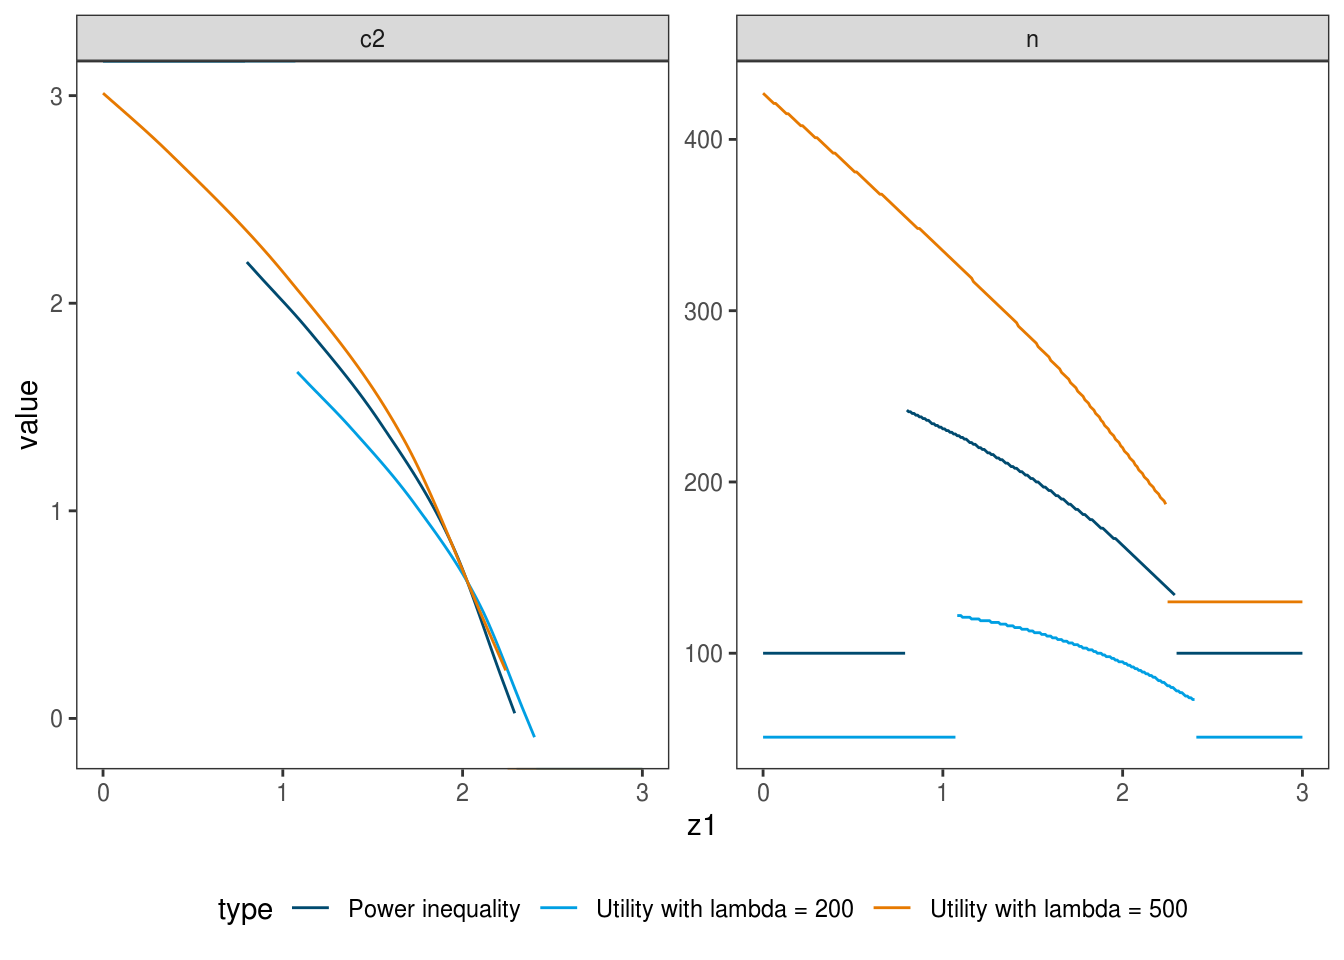
\includegraphics{adoptr-validation-report_files/figure-latex/unnamed-chunk-95-1.pdf}

\hypertarget{variantV_3}{%
\section{Variant V-3, n1-penalty}\label{variantV_3}}

In this case, the influence of the regularization term \texttt{N1()} is investigated.

\hypertarget{objective-12}{%
\subsection{Objective}\label{objective-12}}

In this case, a mixed criterion consisting of expected sample size and
\(n_1\) is minimized.

\begin{Shaded}
\begin{Highlighting}[]
\NormalTok{N1 <-}\StringTok{ }\KeywordTok{N1}\NormalTok{()}

\NormalTok{obj3 <-}\StringTok{ }\ControlFlowTok{function}\NormalTok{(lambda) \{}
  \KeywordTok{composite}\NormalTok{(\{ess }\OperatorTok{+}\StringTok{ }\NormalTok{lambda }\OperatorTok{*}\StringTok{ }\NormalTok{N1\})}
\NormalTok{\}}
\end{Highlighting}
\end{Shaded}

\hypertarget{constraints-12}{%
\subsection{Constraints}\label{constraints-12}}

The inequalities from variant V.1 can still be used.

\hypertarget{initial-design-10}{%
\subsection{Initial Design}\label{initial-design-10}}

The previous initial design with order \(5\) is applied.

\hypertarget{optimization-11}{%
\subsection{Optimization}\label{optimization-11}}

The optimal design is computed for two values of \(\lambda\): 0.05 and 0.2.

\begin{Shaded}
\begin{Highlighting}[]
\NormalTok{opt3_design <-}\StringTok{ }\ControlFlowTok{function}\NormalTok{(lambda) \{}

    \KeywordTok{minimize}\NormalTok{(}
        \KeywordTok{obj3}\NormalTok{(lambda),}
        \KeywordTok{subject_to}\NormalTok{(}
\NormalTok{            toer_cnstr,}
\NormalTok{            pow_cnstr}
\NormalTok{        ),}
        \DataTypeTok{initial_design =} \KeywordTok{init_design}\NormalTok{(}\DecValTok{5}\NormalTok{),}
        \DataTypeTok{opts =}\NormalTok{ opts}
\NormalTok{    )}
\NormalTok{\}}

\NormalTok{opt3 <-}\StringTok{ }\KeywordTok{lapply}\NormalTok{(}\KeywordTok{c}\NormalTok{(.}\DecValTok{05}\NormalTok{, }\FloatTok{.2}\NormalTok{), }\ControlFlowTok{function}\NormalTok{(x) }\KeywordTok{opt3_design}\NormalTok{(x))}
\end{Highlighting}
\end{Shaded}

\hypertarget{test-cases-12}{%
\subsection{Test cases}\label{test-cases-12}}

Check if the optimization algorithm converged in all cases.

\begin{Shaded}
\begin{Highlighting}[]
\NormalTok{iters <-}\StringTok{ }\KeywordTok{sapply}\NormalTok{(opt3, }\ControlFlowTok{function}\NormalTok{(x) x}\OperatorTok{$}\NormalTok{nloptr_return}\OperatorTok{$}\NormalTok{iterations)}

\KeywordTok{print}\NormalTok{(iters)}
\end{Highlighting}
\end{Shaded}

\begin{verbatim}
## [1] 2233 2478
\end{verbatim}

\begin{Shaded}
\begin{Highlighting}[]
\NormalTok{testthat}\OperatorTok{::}\KeywordTok{expect_true}\NormalTok{(}\KeywordTok{all}\NormalTok{(iters }\OperatorTok{<}\StringTok{ }\NormalTok{opts}\OperatorTok{$}\NormalTok{maxeval))}
\end{Highlighting}
\end{Shaded}

Check if the n1 regularizer of the design with higher \(\lambda\) is lower.

\begin{Shaded}
\begin{Highlighting}[]
\NormalTok{testthat}\OperatorTok{::}\KeywordTok{expect_lte}\NormalTok{(}
    \KeywordTok{evaluate}\NormalTok{(N1, opt3[[}\DecValTok{2}\NormalTok{]]}\OperatorTok{$}\NormalTok{design),}
    \KeywordTok{evaluate}\NormalTok{(N1, opt3[[}\DecValTok{1}\NormalTok{]]}\OperatorTok{$}\NormalTok{design)}
\NormalTok{)}


\NormalTok{testthat}\OperatorTok{::}\KeywordTok{expect_lte}\NormalTok{(}
    \KeywordTok{evaluate}\NormalTok{(N1, opt3[[}\DecValTok{1}\NormalTok{]]}\OperatorTok{$}\NormalTok{design),}
    \KeywordTok{evaluate}\NormalTok{(N1, opt1[[}\DecValTok{1}\NormalTok{]]}\OperatorTok{$}\NormalTok{design)}
\NormalTok{)}
\end{Highlighting}
\end{Shaded}

Finally the three designs computed so far are plotted together to allow
comparison.

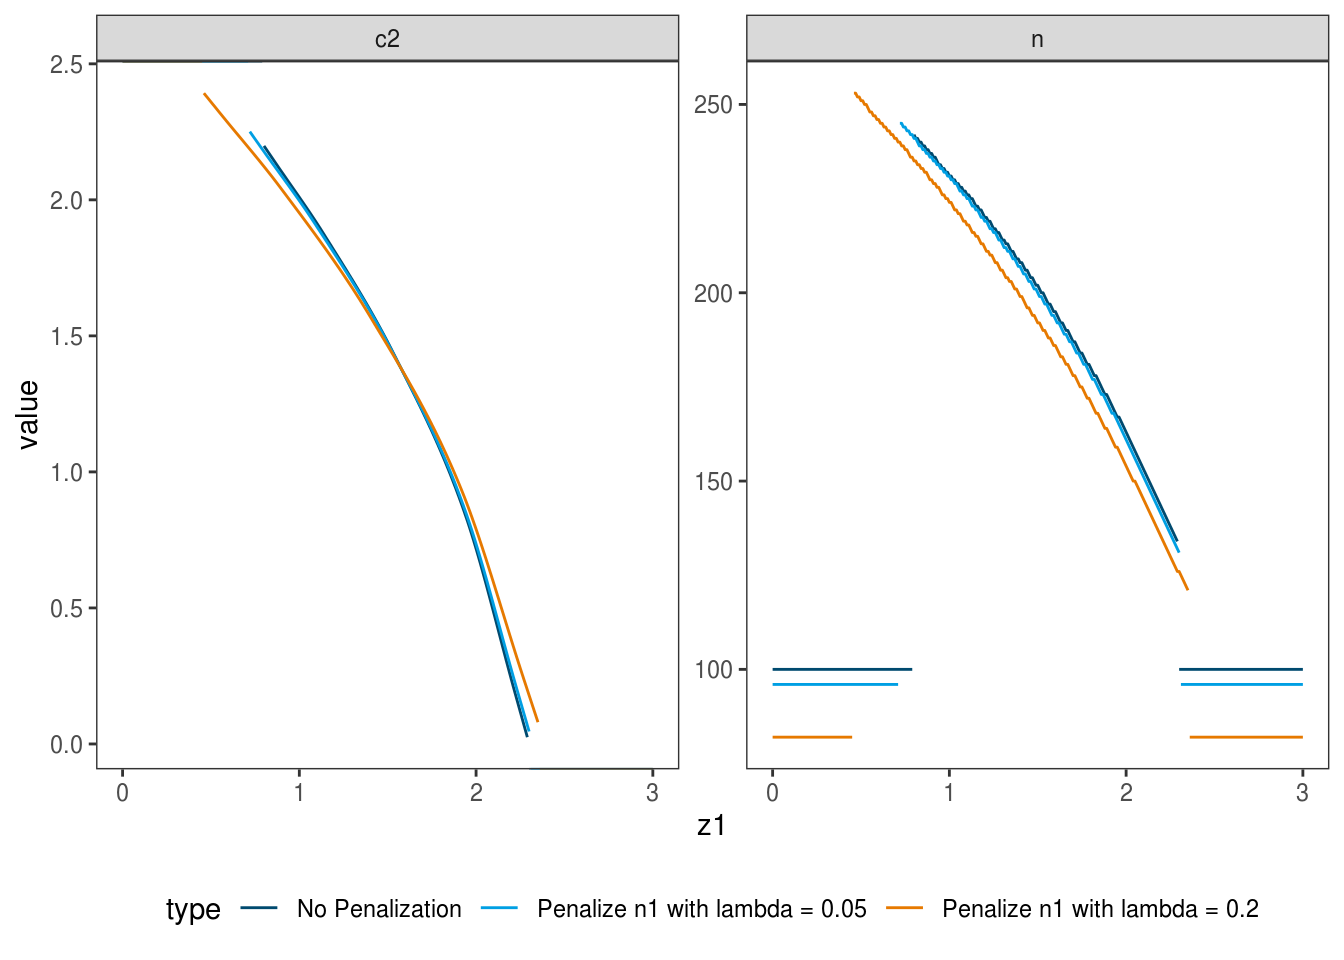
\includegraphics{adoptr-validation-report_files/figure-latex/unnamed-chunk-100-1.pdf}

\hypertarget{variantV_4}{%
\section{Variant V-4, n2-penalty}\label{variantV_4}}

In this case the average over \(n_2\) is penalized by the predefined score
\texttt{AverageN2}.

\hypertarget{objective-13}{%
\subsection{Objective}\label{objective-13}}

In this case, a mixed criterion consisting of expected sample size and
average of \(n_2\) is minimized.

\begin{Shaded}
\begin{Highlighting}[]
\NormalTok{avn2 <-}\StringTok{ }\KeywordTok{AverageN2}\NormalTok{()}

\NormalTok{obj4 <-}\StringTok{ }\ControlFlowTok{function}\NormalTok{(lambda) \{}
  \KeywordTok{composite}\NormalTok{(\{ess }\OperatorTok{+}\StringTok{ }\NormalTok{lambda }\OperatorTok{*}\StringTok{ }\NormalTok{avn2\})}
\NormalTok{\}}
\end{Highlighting}
\end{Shaded}

\hypertarget{constraints-13}{%
\subsection{Constraints}\label{constraints-13}}

The inequalities from variant V.1 can still be used.

\hypertarget{initial-design-11}{%
\subsection{Initial Design}\label{initial-design-11}}

The previous initial design with order \(5\) is applied.

\hypertarget{optimization-12}{%
\subsection{Optimization}\label{optimization-12}}

The optimal design is computed for two values of \(\lambda\): 0.01 and 0.1.

\begin{Shaded}
\begin{Highlighting}[]
\NormalTok{opt4_design <-}\StringTok{ }\ControlFlowTok{function}\NormalTok{(lambda) \{}
    \KeywordTok{minimize}\NormalTok{(}
        \KeywordTok{obj4}\NormalTok{(lambda),}
        \KeywordTok{subject_to}\NormalTok{(}
\NormalTok{            toer_cnstr,}
\NormalTok{            pow_cnstr}
\NormalTok{        ),}
        \DataTypeTok{initial_design =} \KeywordTok{init_design}\NormalTok{(}\DecValTok{5}\NormalTok{),}
        \DataTypeTok{upper_boundary_design =} \KeywordTok{get_upper_boundary_design}\NormalTok{(}\KeywordTok{init_design}\NormalTok{(}\DecValTok{5}\NormalTok{), }\DataTypeTok{c2_buffer=}\DecValTok{3}\NormalTok{),}
        \DataTypeTok{opts =}\NormalTok{ opts}
\NormalTok{    )}
\NormalTok{\}}

\NormalTok{opt4 <-}\StringTok{ }\KeywordTok{lapply}\NormalTok{(}\KeywordTok{c}\NormalTok{(.}\DecValTok{01}\NormalTok{, }\FloatTok{.1}\NormalTok{), }\ControlFlowTok{function}\NormalTok{(x) }\KeywordTok{opt4_design}\NormalTok{(x))}
\end{Highlighting}
\end{Shaded}

\hypertarget{test-cases-13}{%
\subsection{Test cases}\label{test-cases-13}}

Check if the optimization algorithm converged in all cases.

\begin{Shaded}
\begin{Highlighting}[]
\NormalTok{iters <-}\StringTok{ }\KeywordTok{sapply}\NormalTok{(opt4, }\ControlFlowTok{function}\NormalTok{(x) x}\OperatorTok{$}\NormalTok{nloptr_return}\OperatorTok{$}\NormalTok{iterations)}

\KeywordTok{print}\NormalTok{(iters)}
\end{Highlighting}
\end{Shaded}

\begin{verbatim}
## [1] 2196 2376
\end{verbatim}

\begin{Shaded}
\begin{Highlighting}[]
\NormalTok{testthat}\OperatorTok{::}\KeywordTok{expect_true}\NormalTok{(}\KeywordTok{all}\NormalTok{(iters }\OperatorTok{<}\StringTok{ }\NormalTok{opts}\OperatorTok{$}\NormalTok{maxeval))}
\end{Highlighting}
\end{Shaded}

Check if the average \(n_2\) regularizer of the design with
higher \(\lambda\) is lower.

\begin{Shaded}
\begin{Highlighting}[]
\NormalTok{testthat}\OperatorTok{::}\KeywordTok{expect_lte}\NormalTok{(}
    \KeywordTok{evaluate}\NormalTok{(avn2, opt4[[}\DecValTok{2}\NormalTok{]]}\OperatorTok{$}\NormalTok{design),}
    \KeywordTok{evaluate}\NormalTok{(avn2, opt4[[}\DecValTok{1}\NormalTok{]]}\OperatorTok{$}\NormalTok{design)}
\NormalTok{)}


\NormalTok{testthat}\OperatorTok{::}\KeywordTok{expect_lte}\NormalTok{(}
    \KeywordTok{evaluate}\NormalTok{(avn2, opt4[[}\DecValTok{1}\NormalTok{]]}\OperatorTok{$}\NormalTok{design),}
    \KeywordTok{evaluate}\NormalTok{(avn2, opt1[[}\DecValTok{1}\NormalTok{]]}\OperatorTok{$}\NormalTok{design)}
\NormalTok{)}
\end{Highlighting}
\end{Shaded}

Finally the three designs computed so far are plotted together to allow
comparison.

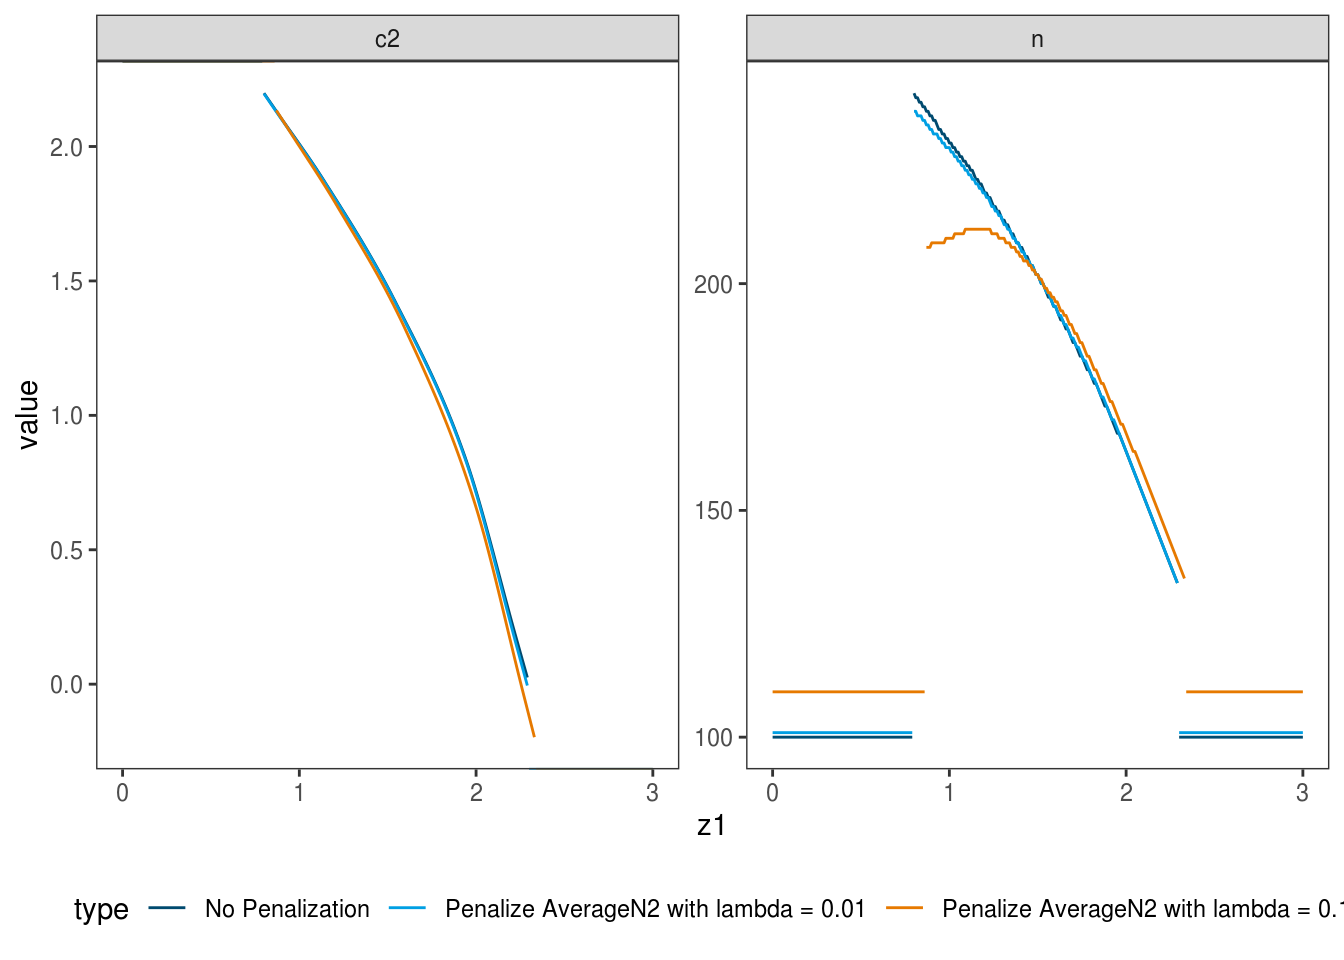
\includegraphics{adoptr-validation-report_files/figure-latex/unnamed-chunk-105-1.pdf}

\bibliography{book.bib,packages.bib}


\end{document}
